\documentclass[twoside]{book}

% Packages required by doxygen
\usepackage{fixltx2e}
\usepackage{calc}
\usepackage{doxygen}
\usepackage[export]{adjustbox} % also loads graphicx
\usepackage{graphicx}
\usepackage[utf8]{inputenc}
\usepackage{makeidx}
\usepackage{multicol}
\usepackage{multirow}
\PassOptionsToPackage{warn}{textcomp}
\usepackage{textcomp}
\usepackage[nointegrals]{wasysym}
\usepackage[table]{xcolor}

% Font selection
\usepackage[T1]{fontenc}
\usepackage[scaled=.90]{helvet}
\usepackage{courier}
\usepackage{amssymb}
\usepackage{sectsty}
\renewcommand{\familydefault}{\sfdefault}
\allsectionsfont{%
  \fontseries{bc}\selectfont%
  \color{darkgray}%
}
\renewcommand{\DoxyLabelFont}{%
  \fontseries{bc}\selectfont%
  \color{darkgray}%
}
\newcommand{\+}{\discretionary{\mbox{\scriptsize$\hookleftarrow$}}{}{}}

% Page & text layout
\usepackage{geometry}
\geometry{%
  a4paper,%
  top=2.5cm,%
  bottom=2.5cm,%
  left=2.5cm,%
  right=2.5cm%
}
\tolerance=750
\hfuzz=15pt
\hbadness=750
\setlength{\emergencystretch}{15pt}
\setlength{\parindent}{0cm}
\setlength{\parskip}{3ex plus 2ex minus 2ex}
\makeatletter
\renewcommand{\paragraph}{%
  \@startsection{paragraph}{4}{0ex}{-1.0ex}{1.0ex}{%
    \normalfont\normalsize\bfseries\SS@parafont%
  }%
}
\renewcommand{\subparagraph}{%
  \@startsection{subparagraph}{5}{0ex}{-1.0ex}{1.0ex}{%
    \normalfont\normalsize\bfseries\SS@subparafont%
  }%
}
\makeatother

% Headers & footers
\usepackage{fancyhdr}
\pagestyle{fancyplain}
\fancyhead[LE]{\fancyplain{}{\bfseries\thepage}}
\fancyhead[CE]{\fancyplain{}{}}
\fancyhead[RE]{\fancyplain{}{\bfseries\leftmark}}
\fancyhead[LO]{\fancyplain{}{\bfseries\rightmark}}
\fancyhead[CO]{\fancyplain{}{}}
\fancyhead[RO]{\fancyplain{}{\bfseries\thepage}}
\fancyfoot[LE]{\fancyplain{}{}}
\fancyfoot[CE]{\fancyplain{}{}}
\fancyfoot[RE]{\fancyplain{}{\bfseries\scriptsize Generated by Doxygen }}
\fancyfoot[LO]{\fancyplain{}{\bfseries\scriptsize Generated by Doxygen }}
\fancyfoot[CO]{\fancyplain{}{}}
\fancyfoot[RO]{\fancyplain{}{}}
\renewcommand{\footrulewidth}{0.4pt}
\renewcommand{\chaptermark}[1]{%
  \markboth{#1}{}%
}
\renewcommand{\sectionmark}[1]{%
  \markright{\thesection\ #1}%
}

% Indices & bibliography
\usepackage{natbib}
\usepackage[titles]{tocloft}
\setcounter{tocdepth}{3}
\setcounter{secnumdepth}{5}
\makeindex

% Hyperlinks (required, but should be loaded last)
\usepackage{ifpdf}
\ifpdf
  \usepackage[pdftex,pagebackref=true]{hyperref}
\else
  \usepackage[ps2pdf,pagebackref=true]{hyperref}
\fi
\hypersetup{%
  colorlinks=true,%
  linkcolor=blue,%
  citecolor=blue,%
  unicode%
}

% Custom commands
\newcommand{\clearemptydoublepage}{%
  \newpage{\pagestyle{empty}\cleardoublepage}%
}

\usepackage{caption}
\captionsetup{labelsep=space,justification=centering,font={bf},singlelinecheck=off,skip=4pt,position=top}

%===== C O N T E N T S =====

\begin{document}

% Titlepage & ToC
\hypersetup{pageanchor=false,
             bookmarksnumbered=true,
             pdfencoding=unicode
            }
\pagenumbering{roman}
\begin{titlepage}
\vspace*{7cm}
\begin{center}%
{\Large Starling Simulation }\\
\vspace*{1cm}
{\large Generated by Doxygen 1.8.11}\\
\end{center}
\end{titlepage}
\clearemptydoublepage
\tableofcontents
\clearemptydoublepage
\pagenumbering{arabic}
\hypersetup{pageanchor=true}

%--- Begin generated contents ---
\chapter{C\+O\+P290 -\/ Starling Simulation -\/ Documentation}
\label{index}\hypertarget{index}{}\hypertarget{index_intro_sec}{}\section{I\+N\+T\+R\+O\+D\+U\+C\+T\+I\+ON}\label{index_intro_sec}
This project is to model and simulate starling murmuration. Objective of this project isto measure from a realistic simulation the average energy spent by each bird, the angular momentum and the force that each bird has to withstand in a typical flight ritual. Starling birds follow number of rules or patterns while foraging. Flocking behavior is one of the most important characteristics shown by starling birds. 
\chapter{Starling-\/\+Simulation}
\label{md_Parametric_Starling-Simulation_README}
\hypertarget{md_Parametric_Starling-Simulation_README}{}
This project is to model and simulate starling murmuration. Objective of this projectisto measure from a realistic simulation the average energy spent by each bird, the angularmomentum and the force that each bird has to withstand in a typical flight ritual. Starlingbirds follow number of rules or patterns while foraging. Flocking behavior is one of the mostimportant characteristics shown by starling birds. 
\chapter{Starling-\/\+Simulation}
\label{md_README}
\hypertarget{md_README}{}
This project is to model and simulate starling murmuration. Objective of this projectisto measure from a realistic simulation the average energy spent by each bird, the angularmomentum and the force that each bird has to withstand in a typical flight ritual. Starlingbirds follow number of rules or patterns while foraging. Flocking behavior is one of the mostimportant characteristics shown by starling birds. 
\chapter{Class Index}
\section{Class List}
Here are the classes, structs, unions and interfaces with brief descriptions\+:\begin{DoxyCompactList}
\item\contentsline{section}{\hyperlink{classboid}{boid} \\*Class for a boid }{\pageref{classboid}}{}
\item\contentsline{section}{\hyperlink{classtuple}{tuple} \\*Class for a tuple }{\pageref{classtuple}}{}
\end{DoxyCompactList}

\chapter{File Index}
\section{File List}
Here is a list of all files with brief descriptions\+:\begin{DoxyCompactList}
\item\contentsline{section}{include/\hyperlink{include_2boid_8h}{boid.\+h} }{\pageref{include_2boid_8h}}{}
\item\contentsline{section}{include/\hyperlink{include_2properties_8h}{properties.\+h} }{\pageref{include_2properties_8h}}{}
\item\contentsline{section}{Parametric/\+Starling-\/\+Simulation/include/\hyperlink{_parametric_2_starling-_simulation_2include_2boid_8h}{boid.\+h} }{\pageref{_parametric_2_starling-_simulation_2include_2boid_8h}}{}
\item\contentsline{section}{Parametric/\+Starling-\/\+Simulation/include/\hyperlink{_parametric_2_starling-_simulation_2include_2properties_8h}{properties.\+h} }{\pageref{_parametric_2_starling-_simulation_2include_2properties_8h}}{}
\item\contentsline{section}{Parametric/\+Starling-\/\+Simulation/src/\hyperlink{_parametric_2_starling-_simulation_2src_2boid_8cpp}{boid.\+cpp} }{\pageref{_parametric_2_starling-_simulation_2src_2boid_8cpp}}{}
\item\contentsline{section}{Parametric/\+Starling-\/\+Simulation/src/\hyperlink{_parametric_2_starling-_simulation_2src_2main_8cpp}{main.\+cpp} }{\pageref{_parametric_2_starling-_simulation_2src_2main_8cpp}}{}
\item\contentsline{section}{Parametric/\+Starling-\/\+Simulation/src/\hyperlink{_parametric_2_starling-_simulation_2src_2properties_8cpp}{properties.\+cpp} }{\pageref{_parametric_2_starling-_simulation_2src_2properties_8cpp}}{}
\item\contentsline{section}{src/\hyperlink{animation_8cpp}{animation.\+cpp} }{\pageref{animation_8cpp}}{}
\item\contentsline{section}{src/\hyperlink{src_2boid_8cpp}{boid.\+cpp} }{\pageref{src_2boid_8cpp}}{}
\item\contentsline{section}{src/\hyperlink{src_2main_8cpp}{main.\+cpp} }{\pageref{src_2main_8cpp}}{}
\item\contentsline{section}{src/\hyperlink{src_2properties_8cpp}{properties.\+cpp} }{\pageref{src_2properties_8cpp}}{}
\end{DoxyCompactList}

\chapter{Class Documentation}
\hypertarget{classboid}{}\section{boid Class Reference}
\label{classboid}\index{boid@{boid}}


class for a boid  




{\ttfamily \#include $<$boid.\+h$>$}



Collaboration diagram for boid\+:
\nopagebreak
\begin{figure}[H]
\begin{center}
\leavevmode
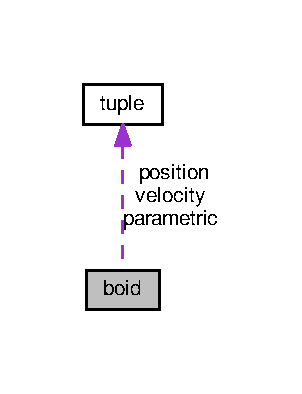
\includegraphics[width=145pt]{classboid__coll__graph}
\end{center}
\end{figure}
\subsection*{Public Member Functions}
\begin{DoxyCompactItemize}
\item 
\hyperlink{classboid_aede77aaa7f5e0473012dd4e251c09a57}{boid} (\hyperlink{classtuple}{tuple} \hyperlink{classboid_aa6af55bf8ffe2a9a19332d12ec632a06}{position}, \hyperlink{classtuple}{tuple} \hyperlink{classboid_a811f5915fa6b7eea89f02b5a455baca4}{velocity})
\begin{DoxyCompactList}\small\item\em Constructor. \end{DoxyCompactList}\item 
\hyperlink{classboid_a1c6b31132d5663db1b623b3c7eb27165}{boid} (\hyperlink{classtuple}{tuple} \hyperlink{classboid_aa6af55bf8ffe2a9a19332d12ec632a06}{position})
\begin{DoxyCompactList}\small\item\em Constructor. \end{DoxyCompactList}\item 
\hyperlink{classboid_a66be2fb9f12b5296304957759ded821a}{boid} ()
\begin{DoxyCompactList}\small\item\em Constructor. \end{DoxyCompactList}\item 
\hyperlink{classboid_aede77aaa7f5e0473012dd4e251c09a57}{boid} (\hyperlink{classtuple}{tuple} \hyperlink{classboid_aa6af55bf8ffe2a9a19332d12ec632a06}{position}, \hyperlink{classtuple}{tuple} \hyperlink{classboid_a811f5915fa6b7eea89f02b5a455baca4}{velocity})
\begin{DoxyCompactList}\small\item\em Constructor. \end{DoxyCompactList}\item 
\hyperlink{classboid_a1c6b31132d5663db1b623b3c7eb27165}{boid} (\hyperlink{classtuple}{tuple} \hyperlink{classboid_aa6af55bf8ffe2a9a19332d12ec632a06}{position})
\begin{DoxyCompactList}\small\item\em Constructor. \end{DoxyCompactList}\item 
\hyperlink{classboid_a66be2fb9f12b5296304957759ded821a}{boid} ()
\begin{DoxyCompactList}\small\item\em Constructor. \end{DoxyCompactList}\end{DoxyCompactItemize}
\subsection*{Public Attributes}
\begin{DoxyCompactItemize}
\item 
\hyperlink{classtuple}{tuple} \hyperlink{classboid_aa6af55bf8ffe2a9a19332d12ec632a06}{position}
\begin{DoxyCompactList}\small\item\em position of the boid \end{DoxyCompactList}\item 
\hyperlink{classtuple}{tuple} \hyperlink{classboid_a811f5915fa6b7eea89f02b5a455baca4}{velocity}
\begin{DoxyCompactList}\small\item\em velocity of the boid \end{DoxyCompactList}\item 
\hyperlink{classtuple}{tuple} \hyperlink{classboid_a38d3b4b3c937c9611505ebc533331276}{parametric}
\end{DoxyCompactItemize}


\subsection{Detailed Description}
class for a boid 

Definition at line 79 of file boid.\+h.



\subsection{Constructor \& Destructor Documentation}
\index{boid@{boid}!boid@{boid}}
\index{boid@{boid}!boid@{boid}}
\subsubsection[{\texorpdfstring{boid(tuple position, tuple velocity)}{boid(tuple position, tuple velocity)}}]{\setlength{\rightskip}{0pt plus 5cm}boid\+::boid (
\begin{DoxyParamCaption}
\item[{{\bf tuple}}]{position, }
\item[{{\bf tuple}}]{velocity}
\end{DoxyParamCaption}
)}\hypertarget{classboid_aede77aaa7f5e0473012dd4e251c09a57}{}\label{classboid_aede77aaa7f5e0473012dd4e251c09a57}


Constructor. 



Definition at line 79 of file boid.\+cpp.

\index{boid@{boid}!boid@{boid}}
\index{boid@{boid}!boid@{boid}}
\subsubsection[{\texorpdfstring{boid(tuple position)}{boid(tuple position)}}]{\setlength{\rightskip}{0pt plus 5cm}boid\+::boid (
\begin{DoxyParamCaption}
\item[{{\bf tuple}}]{position}
\end{DoxyParamCaption}
)}\hypertarget{classboid_a1c6b31132d5663db1b623b3c7eb27165}{}\label{classboid_a1c6b31132d5663db1b623b3c7eb27165}


Constructor. 



Definition at line 93 of file boid.\+cpp.



Here is the call graph for this function\+:
\nopagebreak
\begin{figure}[H]
\begin{center}
\leavevmode
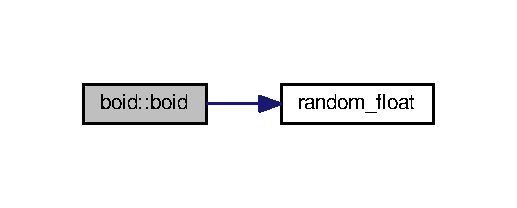
\includegraphics[width=248pt]{classboid_a1c6b31132d5663db1b623b3c7eb27165_cgraph}
\end{center}
\end{figure}


\index{boid@{boid}!boid@{boid}}
\index{boid@{boid}!boid@{boid}}
\subsubsection[{\texorpdfstring{boid()}{boid()}}]{\setlength{\rightskip}{0pt plus 5cm}boid\+::boid (
\begin{DoxyParamCaption}
{}
\end{DoxyParamCaption}
)}\hypertarget{classboid_a66be2fb9f12b5296304957759ded821a}{}\label{classboid_a66be2fb9f12b5296304957759ded821a}


Constructor. 



Definition at line 111 of file boid.\+cpp.



Here is the call graph for this function\+:
\nopagebreak
\begin{figure}[H]
\begin{center}
\leavevmode
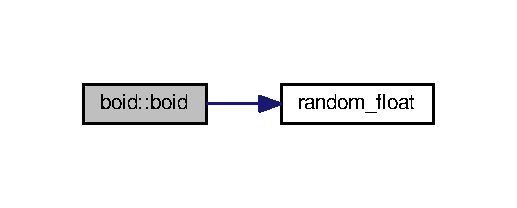
\includegraphics[width=248pt]{classboid_a66be2fb9f12b5296304957759ded821a_cgraph}
\end{center}
\end{figure}


\index{boid@{boid}!boid@{boid}}
\index{boid@{boid}!boid@{boid}}
\subsubsection[{\texorpdfstring{boid(tuple position, tuple velocity)}{boid(tuple position, tuple velocity)}}]{\setlength{\rightskip}{0pt plus 5cm}boid\+::boid (
\begin{DoxyParamCaption}
\item[{{\bf tuple}}]{position, }
\item[{{\bf tuple}}]{velocity}
\end{DoxyParamCaption}
)}\hypertarget{classboid_aede77aaa7f5e0473012dd4e251c09a57}{}\label{classboid_aede77aaa7f5e0473012dd4e251c09a57}


Constructor. 

\index{boid@{boid}!boid@{boid}}
\index{boid@{boid}!boid@{boid}}
\subsubsection[{\texorpdfstring{boid(tuple position)}{boid(tuple position)}}]{\setlength{\rightskip}{0pt plus 5cm}boid\+::boid (
\begin{DoxyParamCaption}
\item[{{\bf tuple}}]{position}
\end{DoxyParamCaption}
)}\hypertarget{classboid_a1c6b31132d5663db1b623b3c7eb27165}{}\label{classboid_a1c6b31132d5663db1b623b3c7eb27165}


Constructor. 

\index{boid@{boid}!boid@{boid}}
\index{boid@{boid}!boid@{boid}}
\subsubsection[{\texorpdfstring{boid()}{boid()}}]{\setlength{\rightskip}{0pt plus 5cm}boid\+::boid (
\begin{DoxyParamCaption}
{}
\end{DoxyParamCaption}
)}\hypertarget{classboid_a66be2fb9f12b5296304957759ded821a}{}\label{classboid_a66be2fb9f12b5296304957759ded821a}


Constructor. 



\subsection{Member Data Documentation}
\index{boid@{boid}!parametric@{parametric}}
\index{parametric@{parametric}!boid@{boid}}
\subsubsection[{\texorpdfstring{parametric}{parametric}}]{\setlength{\rightskip}{0pt plus 5cm}{\bf tuple} boid\+::parametric}\hypertarget{classboid_a38d3b4b3c937c9611505ebc533331276}{}\label{classboid_a38d3b4b3c937c9611505ebc533331276}


Definition at line 71 of file boid.\+h.

\index{boid@{boid}!position@{position}}
\index{position@{position}!boid@{boid}}
\subsubsection[{\texorpdfstring{position}{position}}]{\setlength{\rightskip}{0pt plus 5cm}{\bf tuple} boid\+::position}\hypertarget{classboid_aa6af55bf8ffe2a9a19332d12ec632a06}{}\label{classboid_aa6af55bf8ffe2a9a19332d12ec632a06}


position of the boid 



Definition at line 81 of file boid.\+h.

\index{boid@{boid}!velocity@{velocity}}
\index{velocity@{velocity}!boid@{boid}}
\subsubsection[{\texorpdfstring{velocity}{velocity}}]{\setlength{\rightskip}{0pt plus 5cm}{\bf tuple} boid\+::velocity}\hypertarget{classboid_a811f5915fa6b7eea89f02b5a455baca4}{}\label{classboid_a811f5915fa6b7eea89f02b5a455baca4}


velocity of the boid 



Definition at line 82 of file boid.\+h.



The documentation for this class was generated from the following files\+:\begin{DoxyCompactItemize}
\item 
include/\hyperlink{include_2boid_8h}{boid.\+h}\item 
Parametric/\+Starling-\/\+Simulation/src/\hyperlink{_parametric_2_starling-_simulation_2src_2boid_8cpp}{boid.\+cpp}\end{DoxyCompactItemize}

\hypertarget{classtuple}{}\section{tuple Class Reference}
\label{classtuple}\index{tuple@{tuple}}


class for a tuple  




{\ttfamily \#include $<$boid.\+h$>$}

\subsection*{Public Member Functions}
\begin{DoxyCompactItemize}
\item 
\hyperlink{classtuple_aa764946ab904ef453886051dc107e476}{tuple} (float \hyperlink{classtuple_aa2a27c2f1604d90a8d9f8f786238d29a}{x}, float \hyperlink{classtuple_a7ca83d8377715732d23975e01bf317ec}{y}, float \hyperlink{classtuple_a0d96c11f0004c3682fcfdf9672d9b81d}{z})
\begin{DoxyCompactList}\small\item\em Constructor. \end{DoxyCompactList}\item 
\hyperlink{classtuple_ab9871705086ae665b261bfc8b81f73b0}{tuple} ()
\begin{DoxyCompactList}\small\item\em Constructor. \end{DoxyCompactList}\item 
bool \hyperlink{classtuple_ab57f6f6b41927094633d0d27206181a6}{operator==} (const \hyperlink{classtuple}{tuple} \&rhs)
\begin{DoxyCompactList}\small\item\em bool operator == for vertex\+\_\+2d \end{DoxyCompactList}\item 
bool \hyperlink{classtuple_a121aea0bdaa821cbd870e0de3d161fa3}{operator$<$} (const \hyperlink{classtuple}{tuple} \&rhs)
\begin{DoxyCompactList}\small\item\em bool operator $<$ for vertex\+\_\+2d \end{DoxyCompactList}\item 
\hyperlink{classtuple}{tuple} \hyperlink{classtuple_a828ed2b69e93d38f03d986ea39e10ae6}{operator+} (const \hyperlink{classtuple}{tuple} \&rhs)
\begin{DoxyCompactList}\small\item\em bool operator + for vertex\+\_\+2d \end{DoxyCompactList}\item 
\hyperlink{classtuple}{tuple} \hyperlink{classtuple_aa475aea27ce5ef5fe97f75243ce1bfd3}{operator$\ast$} (const float \&rhs)
\begin{DoxyCompactList}\small\item\em bool operator + for vertex\+\_\+2d \end{DoxyCompactList}\item 
void \hyperlink{classtuple_a83e59acf101fea3b456df1315b04e4b8}{shift\+\_\+it} (\hyperlink{classtuple}{tuple} ref\+\_\+tuple)
\begin{DoxyCompactList}\small\item\em function to shift a tuple wrt to a reference tuple \end{DoxyCompactList}\item 
float \hyperlink{classtuple_a841aaedd191b831b519d3eb7eeae288c}{distance} (\hyperlink{classtuple}{tuple} a)
\begin{DoxyCompactList}\small\item\em function to return the distance b/w to points \end{DoxyCompactList}\item 
float \hyperlink{classtuple_ad60cd51bb5c688f7193fe8f9e6c466b4}{magnitude} ()
\begin{DoxyCompactList}\small\item\em function to return the magnitude of the tuple \end{DoxyCompactList}\item 
void \hyperlink{classtuple_a9a0dddc69bd8da80d05ff0397dee7f68}{make\+\_\+it\+\_\+unit\+\_\+vector} ()
\begin{DoxyCompactList}\small\item\em function to make it unit vector \end{DoxyCompactList}\item 
\hyperlink{classtuple_aa764946ab904ef453886051dc107e476}{tuple} (float \hyperlink{classtuple_aa2a27c2f1604d90a8d9f8f786238d29a}{x}, float \hyperlink{classtuple_a7ca83d8377715732d23975e01bf317ec}{y}, float \hyperlink{classtuple_a0d96c11f0004c3682fcfdf9672d9b81d}{z})
\begin{DoxyCompactList}\small\item\em Constructor. \end{DoxyCompactList}\item 
\hyperlink{classtuple_ab9871705086ae665b261bfc8b81f73b0}{tuple} ()
\begin{DoxyCompactList}\small\item\em Constructor. \end{DoxyCompactList}\item 
bool \hyperlink{classtuple_ab57f6f6b41927094633d0d27206181a6}{operator==} (const \hyperlink{classtuple}{tuple} \&rhs)
\begin{DoxyCompactList}\small\item\em bool operator == for vertex\+\_\+2d \end{DoxyCompactList}\item 
bool \hyperlink{classtuple_a121aea0bdaa821cbd870e0de3d161fa3}{operator$<$} (const \hyperlink{classtuple}{tuple} \&rhs)
\begin{DoxyCompactList}\small\item\em bool operator $<$ for vertex\+\_\+2d \end{DoxyCompactList}\item 
\hyperlink{classtuple}{tuple} \hyperlink{classtuple_a828ed2b69e93d38f03d986ea39e10ae6}{operator+} (const \hyperlink{classtuple}{tuple} \&rhs)
\begin{DoxyCompactList}\small\item\em bool operator + for vertex\+\_\+2d \end{DoxyCompactList}\item 
\hyperlink{classtuple}{tuple} \hyperlink{classtuple_aa475aea27ce5ef5fe97f75243ce1bfd3}{operator$\ast$} (const float \&rhs)
\begin{DoxyCompactList}\small\item\em bool operator + for vertex\+\_\+2d \end{DoxyCompactList}\item 
void \hyperlink{classtuple_a83e59acf101fea3b456df1315b04e4b8}{shift\+\_\+it} (\hyperlink{classtuple}{tuple} ref\+\_\+tuple)
\begin{DoxyCompactList}\small\item\em function to shift a tuple wrt to a reference tuple \end{DoxyCompactList}\item 
float \hyperlink{classtuple_a841aaedd191b831b519d3eb7eeae288c}{distance} (\hyperlink{classtuple}{tuple} a)
\begin{DoxyCompactList}\small\item\em function to return the distance b/w to points \end{DoxyCompactList}\item 
float \hyperlink{classtuple_ad60cd51bb5c688f7193fe8f9e6c466b4}{magnitude} ()
\begin{DoxyCompactList}\small\item\em function to return the magnitude of the tuple \end{DoxyCompactList}\item 
void \hyperlink{classtuple_a9a0dddc69bd8da80d05ff0397dee7f68}{make\+\_\+it\+\_\+unit\+\_\+vector} ()
\begin{DoxyCompactList}\small\item\em function to make it unit vector \end{DoxyCompactList}\end{DoxyCompactItemize}
\subsection*{Public Attributes}
\begin{DoxyCompactItemize}
\item 
float \hyperlink{classtuple_aa2a27c2f1604d90a8d9f8f786238d29a}{x}
\begin{DoxyCompactList}\small\item\em x-\/coordinate of the tuple \end{DoxyCompactList}\item 
float \hyperlink{classtuple_a7ca83d8377715732d23975e01bf317ec}{y}
\begin{DoxyCompactList}\small\item\em y-\/coordinate of the tuple \end{DoxyCompactList}\item 
float \hyperlink{classtuple_a0d96c11f0004c3682fcfdf9672d9b81d}{z}
\begin{DoxyCompactList}\small\item\em z-\/coordinate of the tuple \end{DoxyCompactList}\end{DoxyCompactItemize}


\subsection{Detailed Description}
class for a tuple 

Definition at line 33 of file boid.\+h.



\subsection{Constructor \& Destructor Documentation}
\index{tuple@{tuple}!tuple@{tuple}}
\index{tuple@{tuple}!tuple@{tuple}}
\subsubsection[{\texorpdfstring{tuple(float x, float y, float z)}{tuple(float x, float y, float z)}}]{\setlength{\rightskip}{0pt plus 5cm}tuple\+::tuple (
\begin{DoxyParamCaption}
\item[{float}]{x, }
\item[{float}]{y, }
\item[{float}]{z}
\end{DoxyParamCaption}
)}\hypertarget{classtuple_aa764946ab904ef453886051dc107e476}{}\label{classtuple_aa764946ab904ef453886051dc107e476}


Constructor. 



Definition at line 6 of file boid.\+cpp.

\index{tuple@{tuple}!tuple@{tuple}}
\index{tuple@{tuple}!tuple@{tuple}}
\subsubsection[{\texorpdfstring{tuple()}{tuple()}}]{\setlength{\rightskip}{0pt plus 5cm}tuple\+::tuple (
\begin{DoxyParamCaption}
{}
\end{DoxyParamCaption}
)}\hypertarget{classtuple_ab9871705086ae665b261bfc8b81f73b0}{}\label{classtuple_ab9871705086ae665b261bfc8b81f73b0}


Constructor. 



Definition at line 11 of file boid.\+cpp.

\index{tuple@{tuple}!tuple@{tuple}}
\index{tuple@{tuple}!tuple@{tuple}}
\subsubsection[{\texorpdfstring{tuple(float x, float y, float z)}{tuple(float x, float y, float z)}}]{\setlength{\rightskip}{0pt plus 5cm}tuple\+::tuple (
\begin{DoxyParamCaption}
\item[{float}]{x, }
\item[{float}]{y, }
\item[{float}]{z}
\end{DoxyParamCaption}
)}\hypertarget{classtuple_aa764946ab904ef453886051dc107e476}{}\label{classtuple_aa764946ab904ef453886051dc107e476}


Constructor. 

\index{tuple@{tuple}!tuple@{tuple}}
\index{tuple@{tuple}!tuple@{tuple}}
\subsubsection[{\texorpdfstring{tuple()}{tuple()}}]{\setlength{\rightskip}{0pt plus 5cm}tuple\+::tuple (
\begin{DoxyParamCaption}
{}
\end{DoxyParamCaption}
)}\hypertarget{classtuple_ab9871705086ae665b261bfc8b81f73b0}{}\label{classtuple_ab9871705086ae665b261bfc8b81f73b0}


Constructor. 



\subsection{Member Function Documentation}
\index{tuple@{tuple}!distance@{distance}}
\index{distance@{distance}!tuple@{tuple}}
\subsubsection[{\texorpdfstring{distance(tuple a)}{distance(tuple a)}}]{\setlength{\rightskip}{0pt plus 5cm}float tuple\+::distance (
\begin{DoxyParamCaption}
\item[{{\bf tuple}}]{a}
\end{DoxyParamCaption}
)}\hypertarget{classtuple_a841aaedd191b831b519d3eb7eeae288c}{}\label{classtuple_a841aaedd191b831b519d3eb7eeae288c}


function to return the distance b/w to points 

\index{tuple@{tuple}!distance@{distance}}
\index{distance@{distance}!tuple@{tuple}}
\subsubsection[{\texorpdfstring{distance(tuple a)}{distance(tuple a)}}]{\setlength{\rightskip}{0pt plus 5cm}float tuple\+::distance (
\begin{DoxyParamCaption}
\item[{{\bf tuple}}]{a}
\end{DoxyParamCaption}
)}\hypertarget{classtuple_a841aaedd191b831b519d3eb7eeae288c}{}\label{classtuple_a841aaedd191b831b519d3eb7eeae288c}


function to return the distance b/w to points 



Definition at line 40 of file boid.\+cpp.



Here is the caller graph for this function\+:
\nopagebreak
\begin{figure}[H]
\begin{center}
\leavevmode
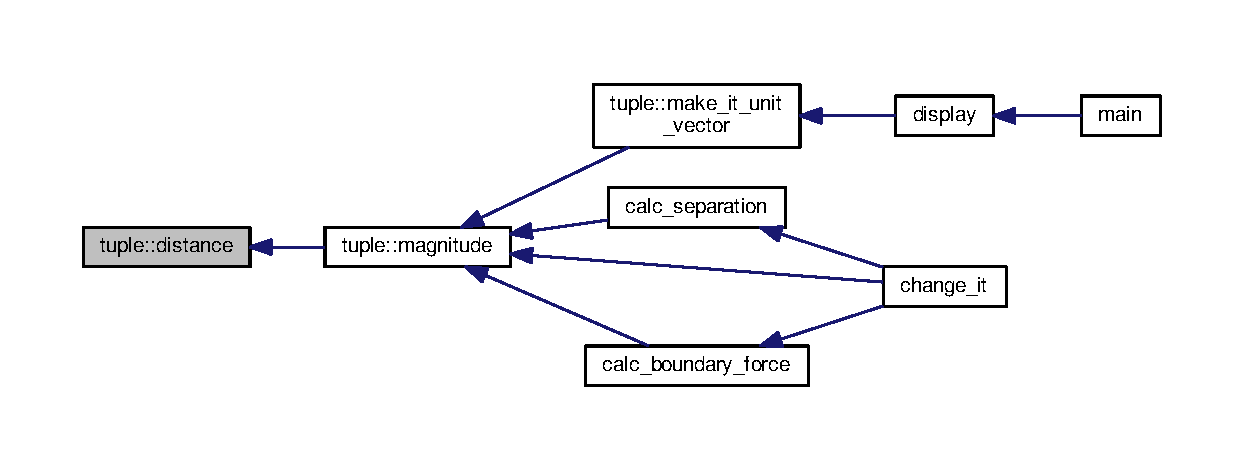
\includegraphics[width=350pt]{classtuple_a841aaedd191b831b519d3eb7eeae288c_icgraph}
\end{center}
\end{figure}


\index{tuple@{tuple}!magnitude@{magnitude}}
\index{magnitude@{magnitude}!tuple@{tuple}}
\subsubsection[{\texorpdfstring{magnitude()}{magnitude()}}]{\setlength{\rightskip}{0pt plus 5cm}float tuple\+::magnitude (
\begin{DoxyParamCaption}
{}
\end{DoxyParamCaption}
)}\hypertarget{classtuple_ad60cd51bb5c688f7193fe8f9e6c466b4}{}\label{classtuple_ad60cd51bb5c688f7193fe8f9e6c466b4}


function to return the magnitude of the tuple 

\index{tuple@{tuple}!magnitude@{magnitude}}
\index{magnitude@{magnitude}!tuple@{tuple}}
\subsubsection[{\texorpdfstring{magnitude()}{magnitude()}}]{\setlength{\rightskip}{0pt plus 5cm}float tuple\+::magnitude (
\begin{DoxyParamCaption}
{}
\end{DoxyParamCaption}
)}\hypertarget{classtuple_ad60cd51bb5c688f7193fe8f9e6c466b4}{}\label{classtuple_ad60cd51bb5c688f7193fe8f9e6c466b4}


function to return the magnitude of the tuple 



Definition at line 49 of file boid.\+cpp.



Here is the call graph for this function\+:
\nopagebreak
\begin{figure}[H]
\begin{center}
\leavevmode
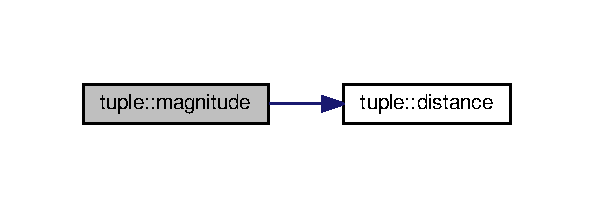
\includegraphics[width=285pt]{classtuple_ad60cd51bb5c688f7193fe8f9e6c466b4_cgraph}
\end{center}
\end{figure}




Here is the caller graph for this function\+:
\nopagebreak
\begin{figure}[H]
\begin{center}
\leavevmode
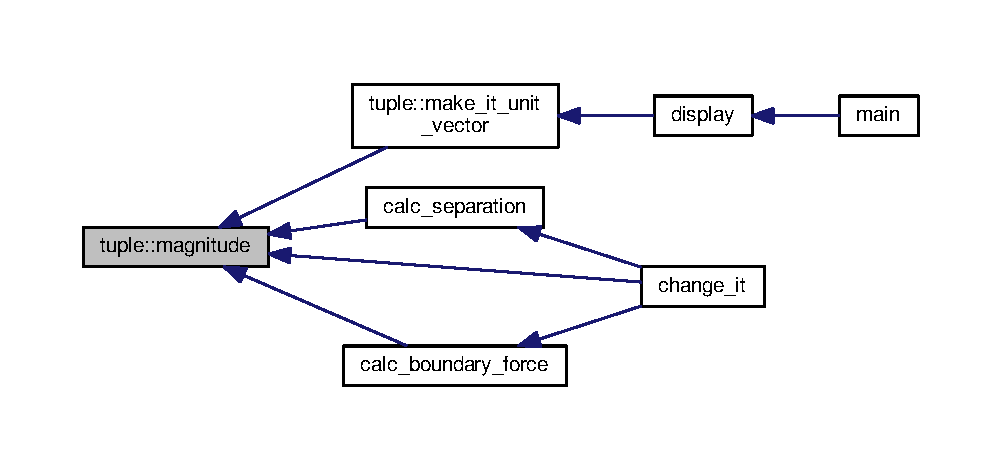
\includegraphics[width=350pt]{classtuple_ad60cd51bb5c688f7193fe8f9e6c466b4_icgraph}
\end{center}
\end{figure}


\index{tuple@{tuple}!make\+\_\+it\+\_\+unit\+\_\+vector@{make\+\_\+it\+\_\+unit\+\_\+vector}}
\index{make\+\_\+it\+\_\+unit\+\_\+vector@{make\+\_\+it\+\_\+unit\+\_\+vector}!tuple@{tuple}}
\subsubsection[{\texorpdfstring{make\+\_\+it\+\_\+unit\+\_\+vector()}{make_it_unit_vector()}}]{\setlength{\rightskip}{0pt plus 5cm}void tuple\+::make\+\_\+it\+\_\+unit\+\_\+vector (
\begin{DoxyParamCaption}
{}
\end{DoxyParamCaption}
)}\hypertarget{classtuple_a9a0dddc69bd8da80d05ff0397dee7f68}{}\label{classtuple_a9a0dddc69bd8da80d05ff0397dee7f68}


function to make it unit vector 

\index{tuple@{tuple}!make\+\_\+it\+\_\+unit\+\_\+vector@{make\+\_\+it\+\_\+unit\+\_\+vector}}
\index{make\+\_\+it\+\_\+unit\+\_\+vector@{make\+\_\+it\+\_\+unit\+\_\+vector}!tuple@{tuple}}
\subsubsection[{\texorpdfstring{make\+\_\+it\+\_\+unit\+\_\+vector()}{make_it_unit_vector()}}]{\setlength{\rightskip}{0pt plus 5cm}void tuple\+::make\+\_\+it\+\_\+unit\+\_\+vector (
\begin{DoxyParamCaption}
{}
\end{DoxyParamCaption}
)}\hypertarget{classtuple_a9a0dddc69bd8da80d05ff0397dee7f68}{}\label{classtuple_a9a0dddc69bd8da80d05ff0397dee7f68}


function to make it unit vector 



Definition at line 71 of file boid.\+cpp.



Here is the call graph for this function\+:
\nopagebreak
\begin{figure}[H]
\begin{center}
\leavevmode
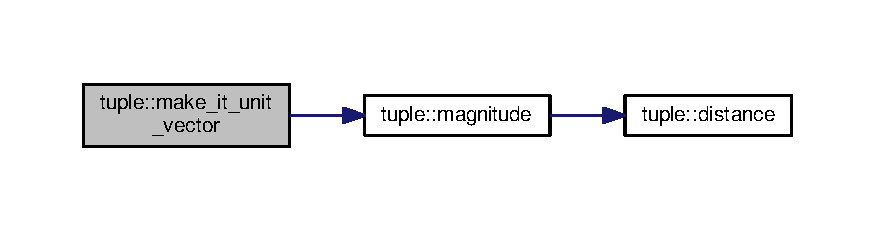
\includegraphics[width=350pt]{classtuple_a9a0dddc69bd8da80d05ff0397dee7f68_cgraph}
\end{center}
\end{figure}




Here is the caller graph for this function\+:
\nopagebreak
\begin{figure}[H]
\begin{center}
\leavevmode
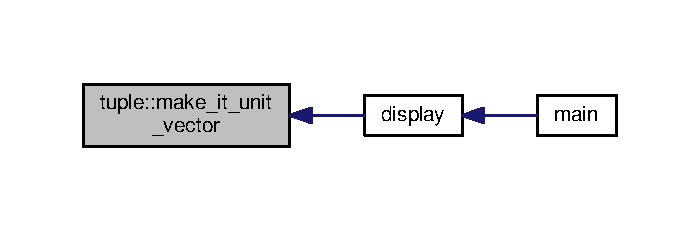
\includegraphics[width=336pt]{classtuple_a9a0dddc69bd8da80d05ff0397dee7f68_icgraph}
\end{center}
\end{figure}


\index{tuple@{tuple}!operator$\ast$@{operator$\ast$}}
\index{operator$\ast$@{operator$\ast$}!tuple@{tuple}}
\subsubsection[{\texorpdfstring{operator$\ast$(const float \&rhs)}{operator*(const float &rhs)}}]{\setlength{\rightskip}{0pt plus 5cm}{\bf tuple} tuple\+::operator$\ast$ (
\begin{DoxyParamCaption}
\item[{const float \&}]{rhs}
\end{DoxyParamCaption}
)}\hypertarget{classtuple_aa475aea27ce5ef5fe97f75243ce1bfd3}{}\label{classtuple_aa475aea27ce5ef5fe97f75243ce1bfd3}


bool operator + for vertex\+\_\+2d 

\index{tuple@{tuple}!operator$\ast$@{operator$\ast$}}
\index{operator$\ast$@{operator$\ast$}!tuple@{tuple}}
\subsubsection[{\texorpdfstring{operator$\ast$(const float \&rhs)}{operator*(const float &rhs)}}]{\setlength{\rightskip}{0pt plus 5cm}{\bf tuple} tuple\+::operator$\ast$ (
\begin{DoxyParamCaption}
\item[{const float \&}]{rhs}
\end{DoxyParamCaption}
)}\hypertarget{classtuple_aa475aea27ce5ef5fe97f75243ce1bfd3}{}\label{classtuple_aa475aea27ce5ef5fe97f75243ce1bfd3}


bool operator + for vertex\+\_\+2d 



Definition at line 30 of file boid.\+cpp.

\index{tuple@{tuple}!operator+@{operator+}}
\index{operator+@{operator+}!tuple@{tuple}}
\subsubsection[{\texorpdfstring{operator+(const tuple \&rhs)}{operator+(const tuple &rhs)}}]{\setlength{\rightskip}{0pt plus 5cm}{\bf tuple} tuple\+::operator+ (
\begin{DoxyParamCaption}
\item[{const {\bf tuple} \&}]{rhs}
\end{DoxyParamCaption}
)}\hypertarget{classtuple_a828ed2b69e93d38f03d986ea39e10ae6}{}\label{classtuple_a828ed2b69e93d38f03d986ea39e10ae6}


bool operator + for vertex\+\_\+2d 

\index{tuple@{tuple}!operator+@{operator+}}
\index{operator+@{operator+}!tuple@{tuple}}
\subsubsection[{\texorpdfstring{operator+(const tuple \&rhs)}{operator+(const tuple &rhs)}}]{\setlength{\rightskip}{0pt plus 5cm}{\bf tuple} tuple\+::operator+ (
\begin{DoxyParamCaption}
\item[{const {\bf tuple} \&}]{rhs}
\end{DoxyParamCaption}
)}\hypertarget{classtuple_a828ed2b69e93d38f03d986ea39e10ae6}{}\label{classtuple_a828ed2b69e93d38f03d986ea39e10ae6}


bool operator + for vertex\+\_\+2d 



Definition at line 21 of file boid.\+cpp.

\index{tuple@{tuple}!operator$<$@{operator$<$}}
\index{operator$<$@{operator$<$}!tuple@{tuple}}
\subsubsection[{\texorpdfstring{operator$<$(const tuple \&rhs)}{operator<(const tuple &rhs)}}]{\setlength{\rightskip}{0pt plus 5cm}bool tuple\+::operator$<$ (
\begin{DoxyParamCaption}
\item[{const {\bf tuple} \&}]{rhs}
\end{DoxyParamCaption}
)}\hypertarget{classtuple_a121aea0bdaa821cbd870e0de3d161fa3}{}\label{classtuple_a121aea0bdaa821cbd870e0de3d161fa3}


bool operator $<$ for vertex\+\_\+2d 

\index{tuple@{tuple}!operator$<$@{operator$<$}}
\index{operator$<$@{operator$<$}!tuple@{tuple}}
\subsubsection[{\texorpdfstring{operator$<$(const tuple \&rhs)}{operator<(const tuple &rhs)}}]{\setlength{\rightskip}{0pt plus 5cm}bool tuple\+::operator$<$ (
\begin{DoxyParamCaption}
\item[{const {\bf tuple} \&}]{rhs}
\end{DoxyParamCaption}
)}\hypertarget{classtuple_a121aea0bdaa821cbd870e0de3d161fa3}{}\label{classtuple_a121aea0bdaa821cbd870e0de3d161fa3}


bool operator $<$ for vertex\+\_\+2d 



Definition at line 56 of file boid.\+cpp.

\index{tuple@{tuple}!operator==@{operator==}}
\index{operator==@{operator==}!tuple@{tuple}}
\subsubsection[{\texorpdfstring{operator==(const tuple \&rhs)}{operator==(const tuple &rhs)}}]{\setlength{\rightskip}{0pt plus 5cm}bool tuple\+::operator== (
\begin{DoxyParamCaption}
\item[{const {\bf tuple} \&}]{rhs}
\end{DoxyParamCaption}
)}\hypertarget{classtuple_ab57f6f6b41927094633d0d27206181a6}{}\label{classtuple_ab57f6f6b41927094633d0d27206181a6}


bool operator == for vertex\+\_\+2d 

\index{tuple@{tuple}!operator==@{operator==}}
\index{operator==@{operator==}!tuple@{tuple}}
\subsubsection[{\texorpdfstring{operator==(const tuple \&rhs)}{operator==(const tuple &rhs)}}]{\setlength{\rightskip}{0pt plus 5cm}bool tuple\+::operator== (
\begin{DoxyParamCaption}
\item[{const {\bf tuple} \&}]{rhs}
\end{DoxyParamCaption}
)}\hypertarget{classtuple_ab57f6f6b41927094633d0d27206181a6}{}\label{classtuple_ab57f6f6b41927094633d0d27206181a6}


bool operator == for vertex\+\_\+2d 



Definition at line 16 of file boid.\+cpp.

\index{tuple@{tuple}!shift\+\_\+it@{shift\+\_\+it}}
\index{shift\+\_\+it@{shift\+\_\+it}!tuple@{tuple}}
\subsubsection[{\texorpdfstring{shift\+\_\+it(tuple ref\+\_\+tuple)}{shift_it(tuple ref_tuple)}}]{\setlength{\rightskip}{0pt plus 5cm}void tuple\+::shift\+\_\+it (
\begin{DoxyParamCaption}
\item[{{\bf tuple}}]{ref\+\_\+tuple}
\end{DoxyParamCaption}
)}\hypertarget{classtuple_a83e59acf101fea3b456df1315b04e4b8}{}\label{classtuple_a83e59acf101fea3b456df1315b04e4b8}


function to shift a tuple wrt to a reference tuple 


\begin{DoxyParams}{Parameters}
{\em ref\+\_\+tuple} & reference tuple chosen as origin \\
\hline
\end{DoxyParams}
\index{tuple@{tuple}!shift\+\_\+it@{shift\+\_\+it}}
\index{shift\+\_\+it@{shift\+\_\+it}!tuple@{tuple}}
\subsubsection[{\texorpdfstring{shift\+\_\+it(tuple ref\+\_\+tuple)}{shift_it(tuple ref_tuple)}}]{\setlength{\rightskip}{0pt plus 5cm}void tuple\+::shift\+\_\+it (
\begin{DoxyParamCaption}
\item[{{\bf tuple}}]{ref\+\_\+tuple}
\end{DoxyParamCaption}
)}\hypertarget{classtuple_a83e59acf101fea3b456df1315b04e4b8}{}\label{classtuple_a83e59acf101fea3b456df1315b04e4b8}


function to shift a tuple wrt to a reference tuple 


\begin{DoxyParams}{Parameters}
{\em ref\+\_\+tuple} & reference tuple chosen as origin \\
\hline
\end{DoxyParams}


Definition at line 66 of file boid.\+cpp.



Here is the caller graph for this function\+:
\nopagebreak
\begin{figure}[H]
\begin{center}
\leavevmode
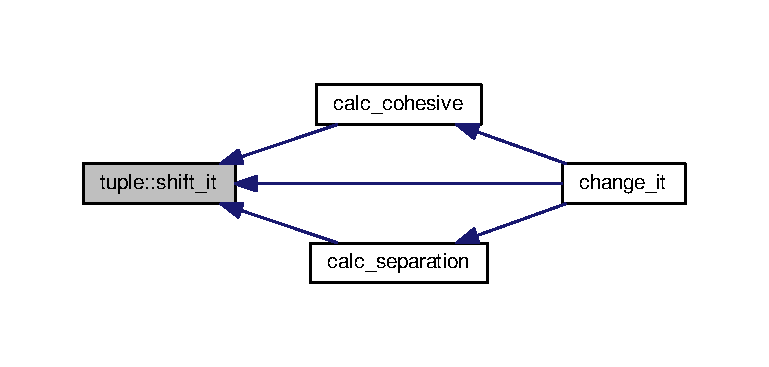
\includegraphics[width=350pt]{classtuple_a83e59acf101fea3b456df1315b04e4b8_icgraph}
\end{center}
\end{figure}




\subsection{Member Data Documentation}
\index{tuple@{tuple}!x@{x}}
\index{x@{x}!tuple@{tuple}}
\subsubsection[{\texorpdfstring{x}{x}}]{\setlength{\rightskip}{0pt plus 5cm}float tuple\+::x}\hypertarget{classtuple_aa2a27c2f1604d90a8d9f8f786238d29a}{}\label{classtuple_aa2a27c2f1604d90a8d9f8f786238d29a}


x-\/coordinate of the tuple 



Definition at line 35 of file boid.\+h.

\index{tuple@{tuple}!y@{y}}
\index{y@{y}!tuple@{tuple}}
\subsubsection[{\texorpdfstring{y}{y}}]{\setlength{\rightskip}{0pt plus 5cm}float tuple\+::y}\hypertarget{classtuple_a7ca83d8377715732d23975e01bf317ec}{}\label{classtuple_a7ca83d8377715732d23975e01bf317ec}


y-\/coordinate of the tuple 



Definition at line 36 of file boid.\+h.

\index{tuple@{tuple}!z@{z}}
\index{z@{z}!tuple@{tuple}}
\subsubsection[{\texorpdfstring{z}{z}}]{\setlength{\rightskip}{0pt plus 5cm}float tuple\+::z}\hypertarget{classtuple_a0d96c11f0004c3682fcfdf9672d9b81d}{}\label{classtuple_a0d96c11f0004c3682fcfdf9672d9b81d}


z-\/coordinate of the tuple 



Definition at line 37 of file boid.\+h.



The documentation for this class was generated from the following files\+:\begin{DoxyCompactItemize}
\item 
include/\hyperlink{include_2boid_8h}{boid.\+h}\item 
Parametric/\+Starling-\/\+Simulation/src/\hyperlink{_parametric_2_starling-_simulation_2src_2boid_8cpp}{boid.\+cpp}\end{DoxyCompactItemize}

\chapter{File Documentation}
\hypertarget{include_2boid_8h}{}\section{include/boid.h File Reference}
\label{include_2boid_8h}\index{include/boid.\+h@{include/boid.\+h}}
This graph shows which files directly or indirectly include this file\+:
\nopagebreak
\begin{figure}[H]
\begin{center}
\leavevmode
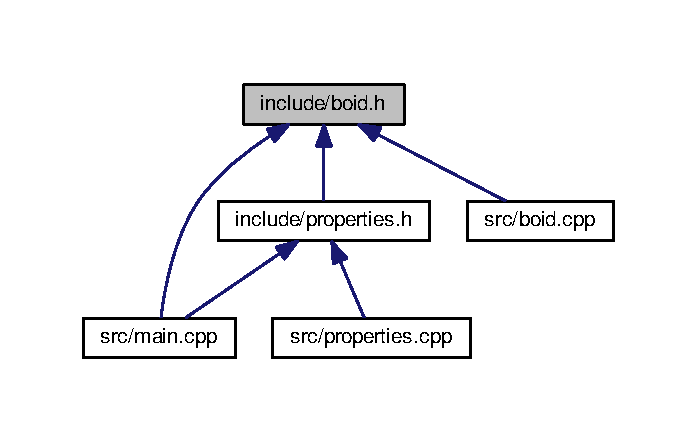
\includegraphics[width=335pt]{include_2boid_8h__dep__incl}
\end{center}
\end{figure}
\subsection*{Classes}
\begin{DoxyCompactItemize}
\item 
class \hyperlink{classtuple}{tuple}
\begin{DoxyCompactList}\small\item\em class for a tuple \end{DoxyCompactList}\item 
class \hyperlink{classboid}{boid}
\begin{DoxyCompactList}\small\item\em class for a boid \end{DoxyCompactList}\end{DoxyCompactItemize}
\subsection*{Macros}
\begin{DoxyCompactItemize}
\item 
\#define \hyperlink{include_2boid_8h_a87b12152029095a33dd01868f0417236}{Xmin}~-\/250.\+0
\item 
\#define \hyperlink{include_2boid_8h_a8fd091040600c54e1b52be58d011ec30}{Xmax}~250.\+0
\item 
\#define \hyperlink{include_2boid_8h_a1653af7892c7f1b3364e1ba87fc75cc1}{Ymin}~-\/250.\+0
\item 
\#define \hyperlink{include_2boid_8h_aaf9edb39f963596bfe86fc184965dcb4}{Ymax}~250.\+0
\item 
\#define \hyperlink{include_2boid_8h_a7ce6b331ba14d64b6306e6975448d23a}{Zmin}~-\/250.\+0
\item 
\#define \hyperlink{include_2boid_8h_a5fe1f9b33875209624ea9b93a0871bd6}{Zmax}~250.\+0
\item 
\#define \hyperlink{include_2boid_8h_ac336537d7a77109375fb312b6c290fcd}{vel\+\_\+\+M\+AX}~10.\+00
\item 
\#define \hyperlink{include_2boid_8h_a882c6328f75739355a7f260afb1c9c1f}{vel\+\_\+\+M\+IN}~-\/10.\+00
\item 
\#define \hyperlink{include_2boid_8h_a276c5a0e984cf60015b27252fe04fe6b}{pb}~push\+\_\+back
\item 
\#define \hyperlink{include_2boid_8h_a3b16749d7ca6b3661d5f3ec81f342650}{freq\+\_\+pankh}~3
\end{DoxyCompactItemize}
\subsection*{Functions}
\begin{DoxyCompactItemize}
\item 
float \hyperlink{include_2boid_8h_a9594488b515ced509126c685b05f880f}{random\+\_\+float} (int mi, int mx)
\item 
\hyperlink{classtuple}{tuple} \hyperlink{include_2boid_8h_a314e8396c9d1befd9b196d3a5adc914f}{cross\+\_\+product} (\hyperlink{classtuple}{tuple} a, \hyperlink{classtuple}{tuple} b)
\item 
float \hyperlink{include_2boid_8h_a5d5b43174fcddb9d32055de5fffd3274}{dot\+\_\+product} (\hyperlink{classtuple}{tuple} a, \hyperlink{classtuple}{tuple} b)
\end{DoxyCompactItemize}


\subsection{Macro Definition Documentation}
\index{include/boid.\+h@{include/boid.\+h}!freq\+\_\+pankh@{freq\+\_\+pankh}}
\index{freq\+\_\+pankh@{freq\+\_\+pankh}!include/boid.\+h@{include/boid.\+h}}
\subsubsection[{\texorpdfstring{freq\+\_\+pankh}{freq_pankh}}]{\setlength{\rightskip}{0pt plus 5cm}\#define freq\+\_\+pankh~3}\hypertarget{include_2boid_8h_a3b16749d7ca6b3661d5f3ec81f342650}{}\label{include_2boid_8h_a3b16749d7ca6b3661d5f3ec81f342650}


Definition at line 14 of file boid.\+h.

\index{include/boid.\+h@{include/boid.\+h}!pb@{pb}}
\index{pb@{pb}!include/boid.\+h@{include/boid.\+h}}
\subsubsection[{\texorpdfstring{pb}{pb}}]{\setlength{\rightskip}{0pt plus 5cm}\#define pb~push\+\_\+back}\hypertarget{include_2boid_8h_a276c5a0e984cf60015b27252fe04fe6b}{}\label{include_2boid_8h_a276c5a0e984cf60015b27252fe04fe6b}


Definition at line 13 of file boid.\+h.

\index{include/boid.\+h@{include/boid.\+h}!vel\+\_\+\+M\+AX@{vel\+\_\+\+M\+AX}}
\index{vel\+\_\+\+M\+AX@{vel\+\_\+\+M\+AX}!include/boid.\+h@{include/boid.\+h}}
\subsubsection[{\texorpdfstring{vel\+\_\+\+M\+AX}{vel_MAX}}]{\setlength{\rightskip}{0pt plus 5cm}\#define vel\+\_\+\+M\+AX~10.\+00}\hypertarget{include_2boid_8h_ac336537d7a77109375fb312b6c290fcd}{}\label{include_2boid_8h_ac336537d7a77109375fb312b6c290fcd}


Definition at line 11 of file boid.\+h.

\index{include/boid.\+h@{include/boid.\+h}!vel\+\_\+\+M\+IN@{vel\+\_\+\+M\+IN}}
\index{vel\+\_\+\+M\+IN@{vel\+\_\+\+M\+IN}!include/boid.\+h@{include/boid.\+h}}
\subsubsection[{\texorpdfstring{vel\+\_\+\+M\+IN}{vel_MIN}}]{\setlength{\rightskip}{0pt plus 5cm}\#define vel\+\_\+\+M\+IN~-\/10.\+00}\hypertarget{include_2boid_8h_a882c6328f75739355a7f260afb1c9c1f}{}\label{include_2boid_8h_a882c6328f75739355a7f260afb1c9c1f}


Definition at line 12 of file boid.\+h.

\index{include/boid.\+h@{include/boid.\+h}!Xmax@{Xmax}}
\index{Xmax@{Xmax}!include/boid.\+h@{include/boid.\+h}}
\subsubsection[{\texorpdfstring{Xmax}{Xmax}}]{\setlength{\rightskip}{0pt plus 5cm}\#define Xmax~250.\+0}\hypertarget{include_2boid_8h_a8fd091040600c54e1b52be58d011ec30}{}\label{include_2boid_8h_a8fd091040600c54e1b52be58d011ec30}


Definition at line 5 of file boid.\+h.

\index{include/boid.\+h@{include/boid.\+h}!Xmin@{Xmin}}
\index{Xmin@{Xmin}!include/boid.\+h@{include/boid.\+h}}
\subsubsection[{\texorpdfstring{Xmin}{Xmin}}]{\setlength{\rightskip}{0pt plus 5cm}\#define Xmin~-\/250.\+0}\hypertarget{include_2boid_8h_a87b12152029095a33dd01868f0417236}{}\label{include_2boid_8h_a87b12152029095a33dd01868f0417236}


Definition at line 4 of file boid.\+h.

\index{include/boid.\+h@{include/boid.\+h}!Ymax@{Ymax}}
\index{Ymax@{Ymax}!include/boid.\+h@{include/boid.\+h}}
\subsubsection[{\texorpdfstring{Ymax}{Ymax}}]{\setlength{\rightskip}{0pt plus 5cm}\#define Ymax~250.\+0}\hypertarget{include_2boid_8h_aaf9edb39f963596bfe86fc184965dcb4}{}\label{include_2boid_8h_aaf9edb39f963596bfe86fc184965dcb4}


Definition at line 7 of file boid.\+h.

\index{include/boid.\+h@{include/boid.\+h}!Ymin@{Ymin}}
\index{Ymin@{Ymin}!include/boid.\+h@{include/boid.\+h}}
\subsubsection[{\texorpdfstring{Ymin}{Ymin}}]{\setlength{\rightskip}{0pt plus 5cm}\#define Ymin~-\/250.\+0}\hypertarget{include_2boid_8h_a1653af7892c7f1b3364e1ba87fc75cc1}{}\label{include_2boid_8h_a1653af7892c7f1b3364e1ba87fc75cc1}


Definition at line 6 of file boid.\+h.

\index{include/boid.\+h@{include/boid.\+h}!Zmax@{Zmax}}
\index{Zmax@{Zmax}!include/boid.\+h@{include/boid.\+h}}
\subsubsection[{\texorpdfstring{Zmax}{Zmax}}]{\setlength{\rightskip}{0pt plus 5cm}\#define Zmax~250.\+0}\hypertarget{include_2boid_8h_a5fe1f9b33875209624ea9b93a0871bd6}{}\label{include_2boid_8h_a5fe1f9b33875209624ea9b93a0871bd6}


Definition at line 9 of file boid.\+h.

\index{include/boid.\+h@{include/boid.\+h}!Zmin@{Zmin}}
\index{Zmin@{Zmin}!include/boid.\+h@{include/boid.\+h}}
\subsubsection[{\texorpdfstring{Zmin}{Zmin}}]{\setlength{\rightskip}{0pt plus 5cm}\#define Zmin~-\/250.\+0}\hypertarget{include_2boid_8h_a7ce6b331ba14d64b6306e6975448d23a}{}\label{include_2boid_8h_a7ce6b331ba14d64b6306e6975448d23a}


Definition at line 8 of file boid.\+h.



\subsection{Function Documentation}
\index{include/boid.\+h@{include/boid.\+h}!cross\+\_\+product@{cross\+\_\+product}}
\index{cross\+\_\+product@{cross\+\_\+product}!include/boid.\+h@{include/boid.\+h}}
\subsubsection[{\texorpdfstring{cross\+\_\+product(tuple a, tuple b)}{cross_product(tuple a, tuple b)}}]{\setlength{\rightskip}{0pt plus 5cm}{\bf tuple} cross\+\_\+product (
\begin{DoxyParamCaption}
\item[{{\bf tuple}}]{a, }
\item[{{\bf tuple}}]{b}
\end{DoxyParamCaption}
)}\hypertarget{include_2boid_8h_a314e8396c9d1befd9b196d3a5adc914f}{}\label{include_2boid_8h_a314e8396c9d1befd9b196d3a5adc914f}


Definition at line 143 of file boid.\+cpp.



Here is the caller graph for this function\+:
\nopagebreak
\begin{figure}[H]
\begin{center}
\leavevmode
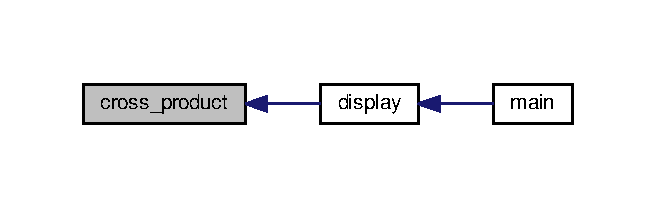
\includegraphics[width=315pt]{include_2boid_8h_a314e8396c9d1befd9b196d3a5adc914f_icgraph}
\end{center}
\end{figure}


\index{include/boid.\+h@{include/boid.\+h}!dot\+\_\+product@{dot\+\_\+product}}
\index{dot\+\_\+product@{dot\+\_\+product}!include/boid.\+h@{include/boid.\+h}}
\subsubsection[{\texorpdfstring{dot\+\_\+product(tuple a, tuple b)}{dot_product(tuple a, tuple b)}}]{\setlength{\rightskip}{0pt plus 5cm}float dot\+\_\+product (
\begin{DoxyParamCaption}
\item[{{\bf tuple}}]{a, }
\item[{{\bf tuple}}]{b}
\end{DoxyParamCaption}
)}\hypertarget{include_2boid_8h_a5d5b43174fcddb9d32055de5fffd3274}{}\label{include_2boid_8h_a5d5b43174fcddb9d32055de5fffd3274}


Definition at line 155 of file boid.\+cpp.

\index{include/boid.\+h@{include/boid.\+h}!random\+\_\+float@{random\+\_\+float}}
\index{random\+\_\+float@{random\+\_\+float}!include/boid.\+h@{include/boid.\+h}}
\subsubsection[{\texorpdfstring{random\+\_\+float(int mi, int mx)}{random_float(int mi, int mx)}}]{\setlength{\rightskip}{0pt plus 5cm}float random\+\_\+float (
\begin{DoxyParamCaption}
\item[{int}]{mi, }
\item[{int}]{mx}
\end{DoxyParamCaption}
)}\hypertarget{include_2boid_8h_a9594488b515ced509126c685b05f880f}{}\label{include_2boid_8h_a9594488b515ced509126c685b05f880f}


Definition at line 133 of file boid.\+cpp.



Here is the caller graph for this function\+:
\nopagebreak
\begin{figure}[H]
\begin{center}
\leavevmode
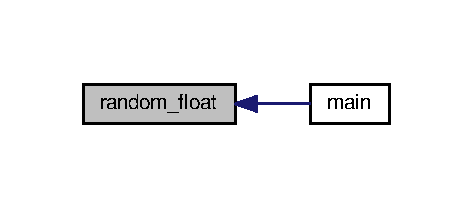
\includegraphics[width=227pt]{include_2boid_8h_a9594488b515ced509126c685b05f880f_icgraph}
\end{center}
\end{figure}



\hypertarget{_parametric_2_starling-_simulation_2include_2boid_8h}{}\section{Parametric/\+Starling-\/\+Simulation/include/boid.h File Reference}
\label{_parametric_2_starling-_simulation_2include_2boid_8h}\index{Parametric/\+Starling-\/\+Simulation/include/boid.\+h@{Parametric/\+Starling-\/\+Simulation/include/boid.\+h}}
This graph shows which files directly or indirectly include this file\+:
\nopagebreak
\begin{figure}[H]
\begin{center}
\leavevmode
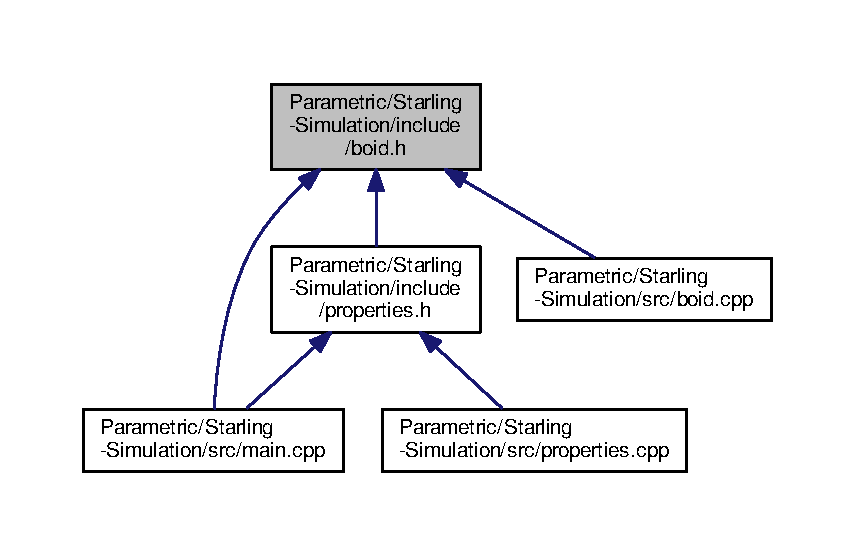
\includegraphics[width=350pt]{_parametric_2_starling-_simulation_2include_2boid_8h__dep__incl}
\end{center}
\end{figure}
\subsection*{Classes}
\begin{DoxyCompactItemize}
\item 
class \hyperlink{classtuple}{tuple}
\begin{DoxyCompactList}\small\item\em class for a tuple \end{DoxyCompactList}\item 
class \hyperlink{classboid}{boid}
\begin{DoxyCompactList}\small\item\em class for a boid \end{DoxyCompactList}\end{DoxyCompactItemize}
\subsection*{Macros}
\begin{DoxyCompactItemize}
\item 
\#define \hyperlink{_parametric_2_starling-_simulation_2include_2boid_8h_a87b12152029095a33dd01868f0417236}{Xmin}~-\/250.\+0
\item 
\#define \hyperlink{_parametric_2_starling-_simulation_2include_2boid_8h_a8fd091040600c54e1b52be58d011ec30}{Xmax}~250.\+0
\item 
\#define \hyperlink{_parametric_2_starling-_simulation_2include_2boid_8h_a1653af7892c7f1b3364e1ba87fc75cc1}{Ymin}~-\/250.\+0
\item 
\#define \hyperlink{_parametric_2_starling-_simulation_2include_2boid_8h_aaf9edb39f963596bfe86fc184965dcb4}{Ymax}~250.\+0
\item 
\#define \hyperlink{_parametric_2_starling-_simulation_2include_2boid_8h_a7ce6b331ba14d64b6306e6975448d23a}{Zmin}~-\/250.\+0
\item 
\#define \hyperlink{_parametric_2_starling-_simulation_2include_2boid_8h_a5fe1f9b33875209624ea9b93a0871bd6}{Zmax}~250.\+0
\item 
\#define \hyperlink{_parametric_2_starling-_simulation_2include_2boid_8h_ac336537d7a77109375fb312b6c290fcd}{vel\+\_\+\+M\+AX}~5.\+00
\item 
\#define \hyperlink{_parametric_2_starling-_simulation_2include_2boid_8h_a882c6328f75739355a7f260afb1c9c1f}{vel\+\_\+\+M\+IN}~-\/5.\+00
\item 
\#define \hyperlink{_parametric_2_starling-_simulation_2include_2boid_8h_a276c5a0e984cf60015b27252fe04fe6b}{pb}~push\+\_\+back
\item 
\#define \hyperlink{_parametric_2_starling-_simulation_2include_2boid_8h_a3b16749d7ca6b3661d5f3ec81f342650}{freq\+\_\+pankh}~3
\end{DoxyCompactItemize}
\subsection*{Functions}
\begin{DoxyCompactItemize}
\item 
float \hyperlink{_parametric_2_starling-_simulation_2include_2boid_8h_a9594488b515ced509126c685b05f880f}{random\+\_\+float} (int mi, int mx)
\item 
\hyperlink{classtuple}{tuple} \hyperlink{_parametric_2_starling-_simulation_2include_2boid_8h_a314e8396c9d1befd9b196d3a5adc914f}{cross\+\_\+product} (\hyperlink{classtuple}{tuple} a, \hyperlink{classtuple}{tuple} b)
\item 
float \hyperlink{_parametric_2_starling-_simulation_2include_2boid_8h_a5d5b43174fcddb9d32055de5fffd3274}{dot\+\_\+product} (\hyperlink{classtuple}{tuple} a, \hyperlink{classtuple}{tuple} b)
\end{DoxyCompactItemize}


\subsection{Macro Definition Documentation}
\index{Parametric/\+Starling-\/\+Simulation/include/boid.\+h@{Parametric/\+Starling-\/\+Simulation/include/boid.\+h}!freq\+\_\+pankh@{freq\+\_\+pankh}}
\index{freq\+\_\+pankh@{freq\+\_\+pankh}!Parametric/\+Starling-\/\+Simulation/include/boid.\+h@{Parametric/\+Starling-\/\+Simulation/include/boid.\+h}}
\subsubsection[{\texorpdfstring{freq\+\_\+pankh}{freq_pankh}}]{\setlength{\rightskip}{0pt plus 5cm}\#define freq\+\_\+pankh~3}\hypertarget{_parametric_2_starling-_simulation_2include_2boid_8h_a3b16749d7ca6b3661d5f3ec81f342650}{}\label{_parametric_2_starling-_simulation_2include_2boid_8h_a3b16749d7ca6b3661d5f3ec81f342650}


Definition at line 14 of file boid.\+h.

\index{Parametric/\+Starling-\/\+Simulation/include/boid.\+h@{Parametric/\+Starling-\/\+Simulation/include/boid.\+h}!pb@{pb}}
\index{pb@{pb}!Parametric/\+Starling-\/\+Simulation/include/boid.\+h@{Parametric/\+Starling-\/\+Simulation/include/boid.\+h}}
\subsubsection[{\texorpdfstring{pb}{pb}}]{\setlength{\rightskip}{0pt plus 5cm}\#define pb~push\+\_\+back}\hypertarget{_parametric_2_starling-_simulation_2include_2boid_8h_a276c5a0e984cf60015b27252fe04fe6b}{}\label{_parametric_2_starling-_simulation_2include_2boid_8h_a276c5a0e984cf60015b27252fe04fe6b}


Definition at line 13 of file boid.\+h.

\index{Parametric/\+Starling-\/\+Simulation/include/boid.\+h@{Parametric/\+Starling-\/\+Simulation/include/boid.\+h}!vel\+\_\+\+M\+AX@{vel\+\_\+\+M\+AX}}
\index{vel\+\_\+\+M\+AX@{vel\+\_\+\+M\+AX}!Parametric/\+Starling-\/\+Simulation/include/boid.\+h@{Parametric/\+Starling-\/\+Simulation/include/boid.\+h}}
\subsubsection[{\texorpdfstring{vel\+\_\+\+M\+AX}{vel_MAX}}]{\setlength{\rightskip}{0pt plus 5cm}\#define vel\+\_\+\+M\+AX~5.\+00}\hypertarget{_parametric_2_starling-_simulation_2include_2boid_8h_ac336537d7a77109375fb312b6c290fcd}{}\label{_parametric_2_starling-_simulation_2include_2boid_8h_ac336537d7a77109375fb312b6c290fcd}


Definition at line 11 of file boid.\+h.

\index{Parametric/\+Starling-\/\+Simulation/include/boid.\+h@{Parametric/\+Starling-\/\+Simulation/include/boid.\+h}!vel\+\_\+\+M\+IN@{vel\+\_\+\+M\+IN}}
\index{vel\+\_\+\+M\+IN@{vel\+\_\+\+M\+IN}!Parametric/\+Starling-\/\+Simulation/include/boid.\+h@{Parametric/\+Starling-\/\+Simulation/include/boid.\+h}}
\subsubsection[{\texorpdfstring{vel\+\_\+\+M\+IN}{vel_MIN}}]{\setlength{\rightskip}{0pt plus 5cm}\#define vel\+\_\+\+M\+IN~-\/5.\+00}\hypertarget{_parametric_2_starling-_simulation_2include_2boid_8h_a882c6328f75739355a7f260afb1c9c1f}{}\label{_parametric_2_starling-_simulation_2include_2boid_8h_a882c6328f75739355a7f260afb1c9c1f}


Definition at line 12 of file boid.\+h.

\index{Parametric/\+Starling-\/\+Simulation/include/boid.\+h@{Parametric/\+Starling-\/\+Simulation/include/boid.\+h}!Xmax@{Xmax}}
\index{Xmax@{Xmax}!Parametric/\+Starling-\/\+Simulation/include/boid.\+h@{Parametric/\+Starling-\/\+Simulation/include/boid.\+h}}
\subsubsection[{\texorpdfstring{Xmax}{Xmax}}]{\setlength{\rightskip}{0pt plus 5cm}\#define Xmax~250.\+0}\hypertarget{_parametric_2_starling-_simulation_2include_2boid_8h_a8fd091040600c54e1b52be58d011ec30}{}\label{_parametric_2_starling-_simulation_2include_2boid_8h_a8fd091040600c54e1b52be58d011ec30}


Definition at line 5 of file boid.\+h.

\index{Parametric/\+Starling-\/\+Simulation/include/boid.\+h@{Parametric/\+Starling-\/\+Simulation/include/boid.\+h}!Xmin@{Xmin}}
\index{Xmin@{Xmin}!Parametric/\+Starling-\/\+Simulation/include/boid.\+h@{Parametric/\+Starling-\/\+Simulation/include/boid.\+h}}
\subsubsection[{\texorpdfstring{Xmin}{Xmin}}]{\setlength{\rightskip}{0pt plus 5cm}\#define Xmin~-\/250.\+0}\hypertarget{_parametric_2_starling-_simulation_2include_2boid_8h_a87b12152029095a33dd01868f0417236}{}\label{_parametric_2_starling-_simulation_2include_2boid_8h_a87b12152029095a33dd01868f0417236}


Definition at line 4 of file boid.\+h.

\index{Parametric/\+Starling-\/\+Simulation/include/boid.\+h@{Parametric/\+Starling-\/\+Simulation/include/boid.\+h}!Ymax@{Ymax}}
\index{Ymax@{Ymax}!Parametric/\+Starling-\/\+Simulation/include/boid.\+h@{Parametric/\+Starling-\/\+Simulation/include/boid.\+h}}
\subsubsection[{\texorpdfstring{Ymax}{Ymax}}]{\setlength{\rightskip}{0pt plus 5cm}\#define Ymax~250.\+0}\hypertarget{_parametric_2_starling-_simulation_2include_2boid_8h_aaf9edb39f963596bfe86fc184965dcb4}{}\label{_parametric_2_starling-_simulation_2include_2boid_8h_aaf9edb39f963596bfe86fc184965dcb4}


Definition at line 7 of file boid.\+h.

\index{Parametric/\+Starling-\/\+Simulation/include/boid.\+h@{Parametric/\+Starling-\/\+Simulation/include/boid.\+h}!Ymin@{Ymin}}
\index{Ymin@{Ymin}!Parametric/\+Starling-\/\+Simulation/include/boid.\+h@{Parametric/\+Starling-\/\+Simulation/include/boid.\+h}}
\subsubsection[{\texorpdfstring{Ymin}{Ymin}}]{\setlength{\rightskip}{0pt plus 5cm}\#define Ymin~-\/250.\+0}\hypertarget{_parametric_2_starling-_simulation_2include_2boid_8h_a1653af7892c7f1b3364e1ba87fc75cc1}{}\label{_parametric_2_starling-_simulation_2include_2boid_8h_a1653af7892c7f1b3364e1ba87fc75cc1}


Definition at line 6 of file boid.\+h.

\index{Parametric/\+Starling-\/\+Simulation/include/boid.\+h@{Parametric/\+Starling-\/\+Simulation/include/boid.\+h}!Zmax@{Zmax}}
\index{Zmax@{Zmax}!Parametric/\+Starling-\/\+Simulation/include/boid.\+h@{Parametric/\+Starling-\/\+Simulation/include/boid.\+h}}
\subsubsection[{\texorpdfstring{Zmax}{Zmax}}]{\setlength{\rightskip}{0pt plus 5cm}\#define Zmax~250.\+0}\hypertarget{_parametric_2_starling-_simulation_2include_2boid_8h_a5fe1f9b33875209624ea9b93a0871bd6}{}\label{_parametric_2_starling-_simulation_2include_2boid_8h_a5fe1f9b33875209624ea9b93a0871bd6}


Definition at line 9 of file boid.\+h.

\index{Parametric/\+Starling-\/\+Simulation/include/boid.\+h@{Parametric/\+Starling-\/\+Simulation/include/boid.\+h}!Zmin@{Zmin}}
\index{Zmin@{Zmin}!Parametric/\+Starling-\/\+Simulation/include/boid.\+h@{Parametric/\+Starling-\/\+Simulation/include/boid.\+h}}
\subsubsection[{\texorpdfstring{Zmin}{Zmin}}]{\setlength{\rightskip}{0pt plus 5cm}\#define Zmin~-\/250.\+0}\hypertarget{_parametric_2_starling-_simulation_2include_2boid_8h_a7ce6b331ba14d64b6306e6975448d23a}{}\label{_parametric_2_starling-_simulation_2include_2boid_8h_a7ce6b331ba14d64b6306e6975448d23a}


Definition at line 8 of file boid.\+h.



\subsection{Function Documentation}
\index{Parametric/\+Starling-\/\+Simulation/include/boid.\+h@{Parametric/\+Starling-\/\+Simulation/include/boid.\+h}!cross\+\_\+product@{cross\+\_\+product}}
\index{cross\+\_\+product@{cross\+\_\+product}!Parametric/\+Starling-\/\+Simulation/include/boid.\+h@{Parametric/\+Starling-\/\+Simulation/include/boid.\+h}}
\subsubsection[{\texorpdfstring{cross\+\_\+product(tuple a, tuple b)}{cross_product(tuple a, tuple b)}}]{\setlength{\rightskip}{0pt plus 5cm}{\bf tuple} cross\+\_\+product (
\begin{DoxyParamCaption}
\item[{{\bf tuple}}]{a, }
\item[{{\bf tuple}}]{b}
\end{DoxyParamCaption}
)}\hypertarget{_parametric_2_starling-_simulation_2include_2boid_8h_a314e8396c9d1befd9b196d3a5adc914f}{}\label{_parametric_2_starling-_simulation_2include_2boid_8h_a314e8396c9d1befd9b196d3a5adc914f}


Definition at line 143 of file boid.\+cpp.

\index{Parametric/\+Starling-\/\+Simulation/include/boid.\+h@{Parametric/\+Starling-\/\+Simulation/include/boid.\+h}!dot\+\_\+product@{dot\+\_\+product}}
\index{dot\+\_\+product@{dot\+\_\+product}!Parametric/\+Starling-\/\+Simulation/include/boid.\+h@{Parametric/\+Starling-\/\+Simulation/include/boid.\+h}}
\subsubsection[{\texorpdfstring{dot\+\_\+product(tuple a, tuple b)}{dot_product(tuple a, tuple b)}}]{\setlength{\rightskip}{0pt plus 5cm}float dot\+\_\+product (
\begin{DoxyParamCaption}
\item[{{\bf tuple}}]{a, }
\item[{{\bf tuple}}]{b}
\end{DoxyParamCaption}
)}\hypertarget{_parametric_2_starling-_simulation_2include_2boid_8h_a5d5b43174fcddb9d32055de5fffd3274}{}\label{_parametric_2_starling-_simulation_2include_2boid_8h_a5d5b43174fcddb9d32055de5fffd3274}


Definition at line 155 of file boid.\+cpp.

\index{Parametric/\+Starling-\/\+Simulation/include/boid.\+h@{Parametric/\+Starling-\/\+Simulation/include/boid.\+h}!random\+\_\+float@{random\+\_\+float}}
\index{random\+\_\+float@{random\+\_\+float}!Parametric/\+Starling-\/\+Simulation/include/boid.\+h@{Parametric/\+Starling-\/\+Simulation/include/boid.\+h}}
\subsubsection[{\texorpdfstring{random\+\_\+float(int mi, int mx)}{random_float(int mi, int mx)}}]{\setlength{\rightskip}{0pt plus 5cm}float random\+\_\+float (
\begin{DoxyParamCaption}
\item[{int}]{mi, }
\item[{int}]{mx}
\end{DoxyParamCaption}
)}\hypertarget{_parametric_2_starling-_simulation_2include_2boid_8h_a9594488b515ced509126c685b05f880f}{}\label{_parametric_2_starling-_simulation_2include_2boid_8h_a9594488b515ced509126c685b05f880f}


Definition at line 133 of file boid.\+cpp.



Here is the caller graph for this function\+:
\nopagebreak
\begin{figure}[H]
\begin{center}
\leavevmode
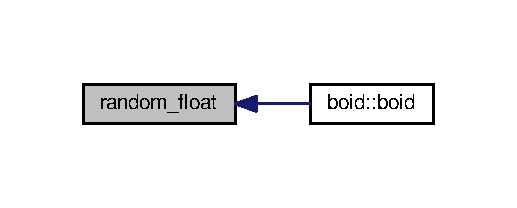
\includegraphics[width=248pt]{_parametric_2_starling-_simulation_2include_2boid_8h_a9594488b515ced509126c685b05f880f_icgraph}
\end{center}
\end{figure}



\hypertarget{include_2properties_8h}{}\section{include/properties.h File Reference}
\label{include_2properties_8h}\index{include/properties.\+h@{include/properties.\+h}}
{\ttfamily \#include \char`\"{}boid.\+h\char`\"{}}\\*
{\ttfamily \#include $<$bits/stdc++.\+h$>$}\\*
Include dependency graph for properties.\+h\+:
\nopagebreak
\begin{figure}[H]
\begin{center}
\leavevmode
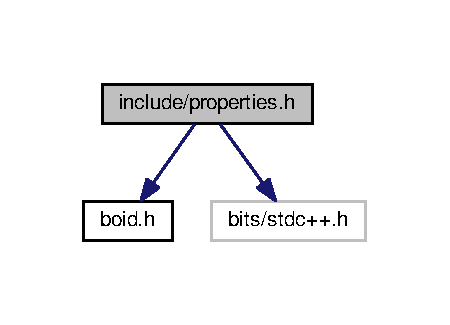
\includegraphics[width=216pt]{include_2properties_8h__incl}
\end{center}
\end{figure}
This graph shows which files directly or indirectly include this file\+:
\nopagebreak
\begin{figure}[H]
\begin{center}
\leavevmode
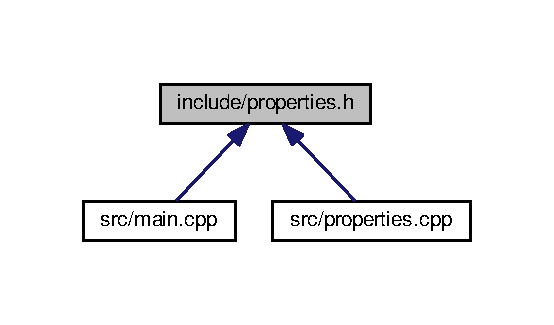
\includegraphics[width=266pt]{include_2properties_8h__dep__incl}
\end{center}
\end{figure}
\subsection*{Functions}
\begin{DoxyCompactItemize}
\item 
void \hyperlink{include_2properties_8h_a0997f2a51d68a3d4a7d8ae247af76cab}{change\+\_\+it} (std\+::vector$<$ \hyperlink{classboid}{boid} $>$ \&\hyperlink{src_2main_8cpp_a1d5a718f1d6b42141bc3a6834be5e420}{v})
\end{DoxyCompactItemize}


\subsection{Function Documentation}
\index{include/properties.\+h@{include/properties.\+h}!change\+\_\+it@{change\+\_\+it}}
\index{change\+\_\+it@{change\+\_\+it}!include/properties.\+h@{include/properties.\+h}}
\subsubsection[{\texorpdfstring{change\+\_\+it(std\+::vector$<$ boid $>$ \&v)}{change_it(std::vector< boid > &v)}}]{\setlength{\rightskip}{0pt plus 5cm}void change\+\_\+it (
\begin{DoxyParamCaption}
\item[{std\+::vector$<$ {\bf boid} $>$ \&}]{v}
\end{DoxyParamCaption}
)}\hypertarget{include_2properties_8h_a0997f2a51d68a3d4a7d8ae247af76cab}{}\label{include_2properties_8h_a0997f2a51d68a3d4a7d8ae247af76cab}


Definition at line 208 of file properties.\+cpp.



Here is the caller graph for this function\+:
\nopagebreak
\begin{figure}[H]
\begin{center}
\leavevmode
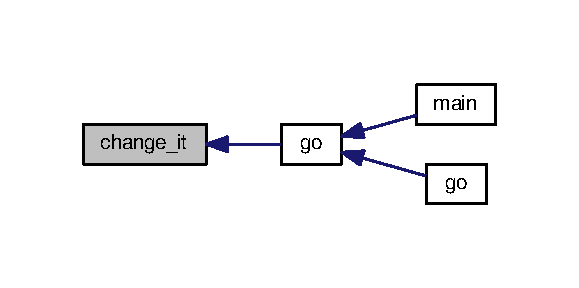
\includegraphics[width=278pt]{include_2properties_8h_a0997f2a51d68a3d4a7d8ae247af76cab_icgraph}
\end{center}
\end{figure}



\hypertarget{_parametric_2_starling-_simulation_2include_2properties_8h}{}\section{Parametric/\+Starling-\/\+Simulation/include/properties.h File Reference}
\label{_parametric_2_starling-_simulation_2include_2properties_8h}\index{Parametric/\+Starling-\/\+Simulation/include/properties.\+h@{Parametric/\+Starling-\/\+Simulation/include/properties.\+h}}
{\ttfamily \#include \char`\"{}boid.\+h\char`\"{}}\\*
{\ttfamily \#include $<$bits/stdc++.\+h$>$}\\*
Include dependency graph for properties.\+h\+:
\nopagebreak
\begin{figure}[H]
\begin{center}
\leavevmode
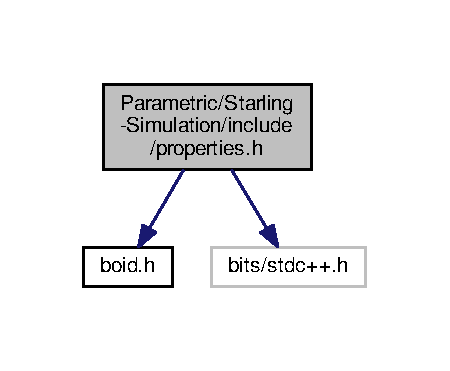
\includegraphics[width=216pt]{_parametric_2_starling-_simulation_2include_2properties_8h__incl}
\end{center}
\end{figure}
This graph shows which files directly or indirectly include this file\+:
\nopagebreak
\begin{figure}[H]
\begin{center}
\leavevmode
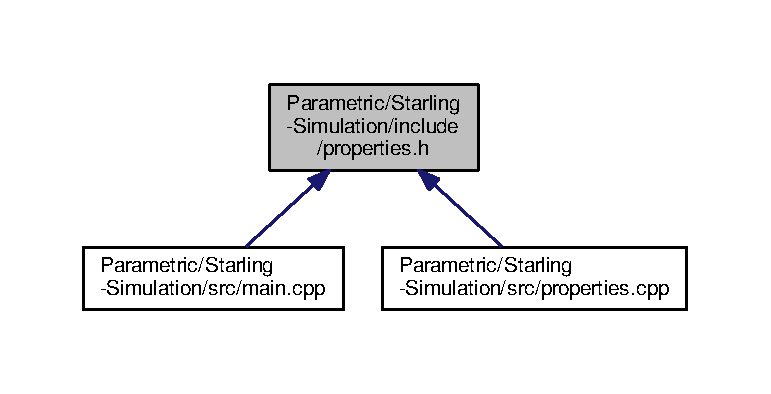
\includegraphics[width=350pt]{_parametric_2_starling-_simulation_2include_2properties_8h__dep__incl}
\end{center}
\end{figure}
\subsection*{Functions}
\begin{DoxyCompactItemize}
\item 
void \hyperlink{_parametric_2_starling-_simulation_2include_2properties_8h_a0997f2a51d68a3d4a7d8ae247af76cab}{change\+\_\+it} (std\+::vector$<$ \hyperlink{classboid}{boid} $>$ \&\hyperlink{src_2main_8cpp_a1d5a718f1d6b42141bc3a6834be5e420}{v})
\end{DoxyCompactItemize}


\subsection{Function Documentation}
\index{Parametric/\+Starling-\/\+Simulation/include/properties.\+h@{Parametric/\+Starling-\/\+Simulation/include/properties.\+h}!change\+\_\+it@{change\+\_\+it}}
\index{change\+\_\+it@{change\+\_\+it}!Parametric/\+Starling-\/\+Simulation/include/properties.\+h@{Parametric/\+Starling-\/\+Simulation/include/properties.\+h}}
\subsubsection[{\texorpdfstring{change\+\_\+it(std\+::vector$<$ boid $>$ \&v)}{change_it(std::vector< boid > &v)}}]{\setlength{\rightskip}{0pt plus 5cm}void change\+\_\+it (
\begin{DoxyParamCaption}
\item[{std\+::vector$<$ {\bf boid} $>$ \&}]{v}
\end{DoxyParamCaption}
)}\hypertarget{_parametric_2_starling-_simulation_2include_2properties_8h_a0997f2a51d68a3d4a7d8ae247af76cab}{}\label{_parametric_2_starling-_simulation_2include_2properties_8h_a0997f2a51d68a3d4a7d8ae247af76cab}


Definition at line 208 of file properties.\+cpp.



Here is the call graph for this function\+:
\nopagebreak
\begin{figure}[H]
\begin{center}
\leavevmode
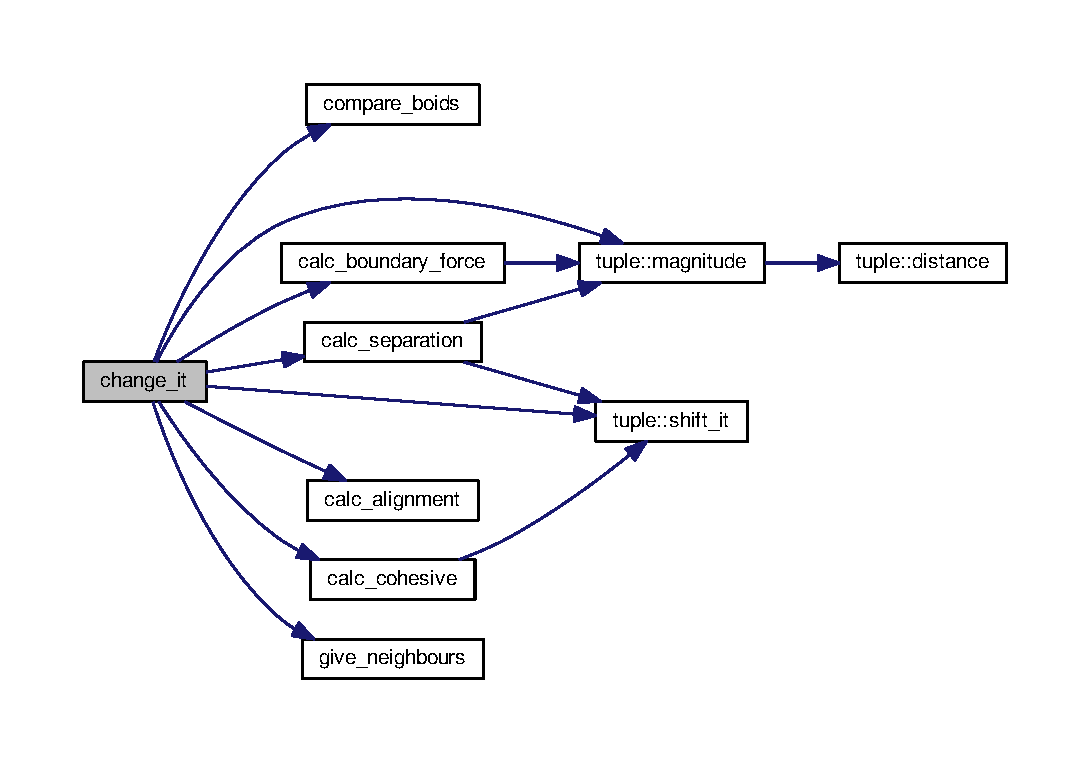
\includegraphics[width=350pt]{_parametric_2_starling-_simulation_2include_2properties_8h_a0997f2a51d68a3d4a7d8ae247af76cab_cgraph}
\end{center}
\end{figure}



\hypertarget{_parametric_2_starling-_simulation_2_r_e_a_d_m_e_8md}{}\section{Parametric/\+Starling-\/\+Simulation/\+R\+E\+A\+D\+ME.md File Reference}
\label{_parametric_2_starling-_simulation_2_r_e_a_d_m_e_8md}\index{Parametric/\+Starling-\/\+Simulation/\+R\+E\+A\+D\+M\+E.\+md@{Parametric/\+Starling-\/\+Simulation/\+R\+E\+A\+D\+M\+E.\+md}}

\hypertarget{_r_e_a_d_m_e_8md}{}\section{R\+E\+A\+D\+M\+E.\+md File Reference}
\label{_r_e_a_d_m_e_8md}\index{R\+E\+A\+D\+M\+E.\+md@{R\+E\+A\+D\+M\+E.\+md}}

\hypertarget{_parametric_2_starling-_simulation_2src_2boid_8cpp}{}\section{Parametric/\+Starling-\/\+Simulation/src/boid.cpp File Reference}
\label{_parametric_2_starling-_simulation_2src_2boid_8cpp}\index{Parametric/\+Starling-\/\+Simulation/src/boid.\+cpp@{Parametric/\+Starling-\/\+Simulation/src/boid.\+cpp}}
{\ttfamily \#include \char`\"{}../include/boid.\+h\char`\"{}}\\*
{\ttfamily \#include $<$bits/stdc++.\+h$>$}\\*
Include dependency graph for boid.\+cpp\+:
\nopagebreak
\begin{figure}[H]
\begin{center}
\leavevmode
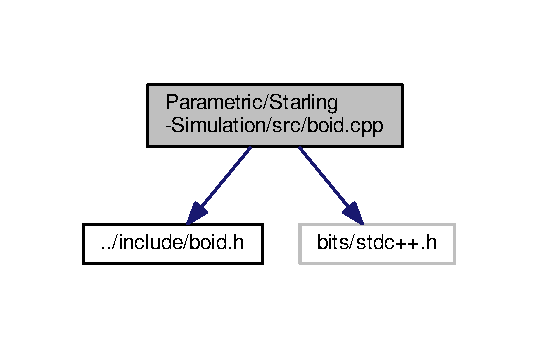
\includegraphics[width=258pt]{_parametric_2_starling-_simulation_2src_2boid_8cpp__incl}
\end{center}
\end{figure}
\subsection*{Macros}
\begin{DoxyCompactItemize}
\item 
\#define \hyperlink{_parametric_2_starling-_simulation_2src_2boid_8cpp_ab53328405fd9ba89990d9426d0e6389e}{eps}~0.\+000001
\end{DoxyCompactItemize}
\subsection*{Functions}
\begin{DoxyCompactItemize}
\item 
float \hyperlink{_parametric_2_starling-_simulation_2src_2boid_8cpp_a9594488b515ced509126c685b05f880f}{random\+\_\+float} (int mi, int mx)
\item 
\hyperlink{classtuple}{tuple} \hyperlink{_parametric_2_starling-_simulation_2src_2boid_8cpp_a314e8396c9d1befd9b196d3a5adc914f}{cross\+\_\+product} (\hyperlink{classtuple}{tuple} a, \hyperlink{classtuple}{tuple} b)
\item 
float \hyperlink{_parametric_2_starling-_simulation_2src_2boid_8cpp_a5d5b43174fcddb9d32055de5fffd3274}{dot\+\_\+product} (\hyperlink{classtuple}{tuple} a, \hyperlink{classtuple}{tuple} b)
\end{DoxyCompactItemize}


\subsection{Macro Definition Documentation}
\index{Parametric/\+Starling-\/\+Simulation/src/boid.\+cpp@{Parametric/\+Starling-\/\+Simulation/src/boid.\+cpp}!eps@{eps}}
\index{eps@{eps}!Parametric/\+Starling-\/\+Simulation/src/boid.\+cpp@{Parametric/\+Starling-\/\+Simulation/src/boid.\+cpp}}
\subsubsection[{\texorpdfstring{eps}{eps}}]{\setlength{\rightskip}{0pt plus 5cm}\#define eps~0.\+000001}\hypertarget{_parametric_2_starling-_simulation_2src_2boid_8cpp_ab53328405fd9ba89990d9426d0e6389e}{}\label{_parametric_2_starling-_simulation_2src_2boid_8cpp_ab53328405fd9ba89990d9426d0e6389e}


Definition at line 2 of file boid.\+cpp.



\subsection{Function Documentation}
\index{Parametric/\+Starling-\/\+Simulation/src/boid.\+cpp@{Parametric/\+Starling-\/\+Simulation/src/boid.\+cpp}!cross\+\_\+product@{cross\+\_\+product}}
\index{cross\+\_\+product@{cross\+\_\+product}!Parametric/\+Starling-\/\+Simulation/src/boid.\+cpp@{Parametric/\+Starling-\/\+Simulation/src/boid.\+cpp}}
\subsubsection[{\texorpdfstring{cross\+\_\+product(tuple a, tuple b)}{cross_product(tuple a, tuple b)}}]{\setlength{\rightskip}{0pt plus 5cm}{\bf tuple} cross\+\_\+product (
\begin{DoxyParamCaption}
\item[{{\bf tuple}}]{a, }
\item[{{\bf tuple}}]{b}
\end{DoxyParamCaption}
)}\hypertarget{_parametric_2_starling-_simulation_2src_2boid_8cpp_a314e8396c9d1befd9b196d3a5adc914f}{}\label{_parametric_2_starling-_simulation_2src_2boid_8cpp_a314e8396c9d1befd9b196d3a5adc914f}


Definition at line 143 of file boid.\+cpp.

\index{Parametric/\+Starling-\/\+Simulation/src/boid.\+cpp@{Parametric/\+Starling-\/\+Simulation/src/boid.\+cpp}!dot\+\_\+product@{dot\+\_\+product}}
\index{dot\+\_\+product@{dot\+\_\+product}!Parametric/\+Starling-\/\+Simulation/src/boid.\+cpp@{Parametric/\+Starling-\/\+Simulation/src/boid.\+cpp}}
\subsubsection[{\texorpdfstring{dot\+\_\+product(tuple a, tuple b)}{dot_product(tuple a, tuple b)}}]{\setlength{\rightskip}{0pt plus 5cm}float dot\+\_\+product (
\begin{DoxyParamCaption}
\item[{{\bf tuple}}]{a, }
\item[{{\bf tuple}}]{b}
\end{DoxyParamCaption}
)}\hypertarget{_parametric_2_starling-_simulation_2src_2boid_8cpp_a5d5b43174fcddb9d32055de5fffd3274}{}\label{_parametric_2_starling-_simulation_2src_2boid_8cpp_a5d5b43174fcddb9d32055de5fffd3274}


Definition at line 155 of file boid.\+cpp.

\index{Parametric/\+Starling-\/\+Simulation/src/boid.\+cpp@{Parametric/\+Starling-\/\+Simulation/src/boid.\+cpp}!random\+\_\+float@{random\+\_\+float}}
\index{random\+\_\+float@{random\+\_\+float}!Parametric/\+Starling-\/\+Simulation/src/boid.\+cpp@{Parametric/\+Starling-\/\+Simulation/src/boid.\+cpp}}
\subsubsection[{\texorpdfstring{random\+\_\+float(int mi, int mx)}{random_float(int mi, int mx)}}]{\setlength{\rightskip}{0pt plus 5cm}float random\+\_\+float (
\begin{DoxyParamCaption}
\item[{int}]{mi, }
\item[{int}]{mx}
\end{DoxyParamCaption}
)}\hypertarget{_parametric_2_starling-_simulation_2src_2boid_8cpp_a9594488b515ced509126c685b05f880f}{}\label{_parametric_2_starling-_simulation_2src_2boid_8cpp_a9594488b515ced509126c685b05f880f}


Definition at line 133 of file boid.\+cpp.



Here is the caller graph for this function\+:
\nopagebreak
\begin{figure}[H]
\begin{center}
\leavevmode
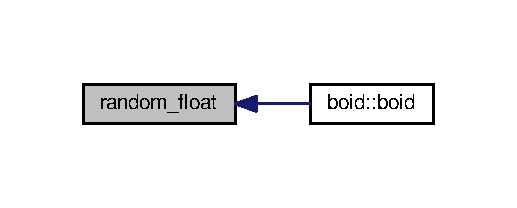
\includegraphics[width=248pt]{_parametric_2_starling-_simulation_2src_2boid_8cpp_a9594488b515ced509126c685b05f880f_icgraph}
\end{center}
\end{figure}



\hypertarget{src_2boid_8cpp}{}\section{src/boid.cpp File Reference}
\label{src_2boid_8cpp}\index{src/boid.\+cpp@{src/boid.\+cpp}}
{\ttfamily \#include \char`\"{}../include/boid.\+h\char`\"{}}\\*
{\ttfamily \#include $<$bits/stdc++.\+h$>$}\\*
Include dependency graph for boid.\+cpp\+:
\nopagebreak
\begin{figure}[H]
\begin{center}
\leavevmode
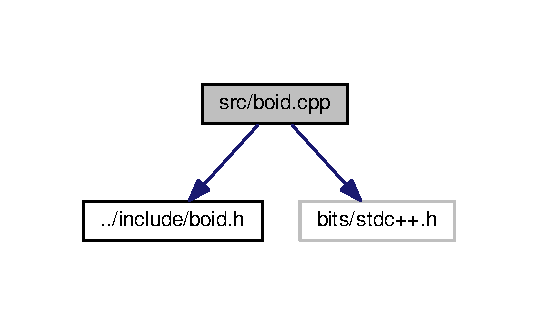
\includegraphics[width=258pt]{src_2boid_8cpp__incl}
\end{center}
\end{figure}
\subsection*{Macros}
\begin{DoxyCompactItemize}
\item 
\#define \hyperlink{src_2boid_8cpp_ab53328405fd9ba89990d9426d0e6389e}{eps}~0.\+000001
\end{DoxyCompactItemize}
\subsection*{Functions}
\begin{DoxyCompactItemize}
\item 
float \hyperlink{src_2boid_8cpp_a9594488b515ced509126c685b05f880f}{random\+\_\+float} (int mi, int mx)
\item 
\hyperlink{classtuple}{tuple} \hyperlink{src_2boid_8cpp_a314e8396c9d1befd9b196d3a5adc914f}{cross\+\_\+product} (\hyperlink{classtuple}{tuple} a, \hyperlink{classtuple}{tuple} b)
\item 
float \hyperlink{src_2boid_8cpp_a5d5b43174fcddb9d32055de5fffd3274}{dot\+\_\+product} (\hyperlink{classtuple}{tuple} a, \hyperlink{classtuple}{tuple} b)
\end{DoxyCompactItemize}


\subsection{Macro Definition Documentation}
\index{src/boid.\+cpp@{src/boid.\+cpp}!eps@{eps}}
\index{eps@{eps}!src/boid.\+cpp@{src/boid.\+cpp}}
\subsubsection[{\texorpdfstring{eps}{eps}}]{\setlength{\rightskip}{0pt plus 5cm}\#define eps~0.\+000001}\hypertarget{src_2boid_8cpp_ab53328405fd9ba89990d9426d0e6389e}{}\label{src_2boid_8cpp_ab53328405fd9ba89990d9426d0e6389e}


Definition at line 2 of file boid.\+cpp.



\subsection{Function Documentation}
\index{src/boid.\+cpp@{src/boid.\+cpp}!cross\+\_\+product@{cross\+\_\+product}}
\index{cross\+\_\+product@{cross\+\_\+product}!src/boid.\+cpp@{src/boid.\+cpp}}
\subsubsection[{\texorpdfstring{cross\+\_\+product(tuple a, tuple b)}{cross_product(tuple a, tuple b)}}]{\setlength{\rightskip}{0pt plus 5cm}{\bf tuple} cross\+\_\+product (
\begin{DoxyParamCaption}
\item[{{\bf tuple}}]{a, }
\item[{{\bf tuple}}]{b}
\end{DoxyParamCaption}
)}\hypertarget{src_2boid_8cpp_a314e8396c9d1befd9b196d3a5adc914f}{}\label{src_2boid_8cpp_a314e8396c9d1befd9b196d3a5adc914f}


Definition at line 121 of file boid.\+cpp.



Here is the caller graph for this function\+:
\nopagebreak
\begin{figure}[H]
\begin{center}
\leavevmode
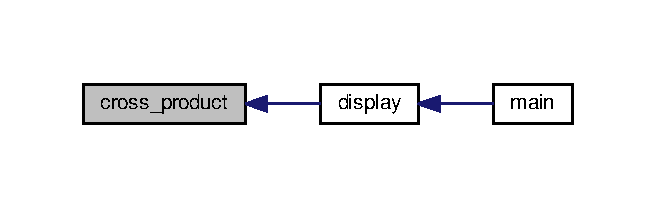
\includegraphics[width=315pt]{src_2boid_8cpp_a314e8396c9d1befd9b196d3a5adc914f_icgraph}
\end{center}
\end{figure}


\index{src/boid.\+cpp@{src/boid.\+cpp}!dot\+\_\+product@{dot\+\_\+product}}
\index{dot\+\_\+product@{dot\+\_\+product}!src/boid.\+cpp@{src/boid.\+cpp}}
\subsubsection[{\texorpdfstring{dot\+\_\+product(tuple a, tuple b)}{dot_product(tuple a, tuple b)}}]{\setlength{\rightskip}{0pt plus 5cm}float dot\+\_\+product (
\begin{DoxyParamCaption}
\item[{{\bf tuple}}]{a, }
\item[{{\bf tuple}}]{b}
\end{DoxyParamCaption}
)}\hypertarget{src_2boid_8cpp_a5d5b43174fcddb9d32055de5fffd3274}{}\label{src_2boid_8cpp_a5d5b43174fcddb9d32055de5fffd3274}


Definition at line 133 of file boid.\+cpp.

\index{src/boid.\+cpp@{src/boid.\+cpp}!random\+\_\+float@{random\+\_\+float}}
\index{random\+\_\+float@{random\+\_\+float}!src/boid.\+cpp@{src/boid.\+cpp}}
\subsubsection[{\texorpdfstring{random\+\_\+float(int mi, int mx)}{random_float(int mi, int mx)}}]{\setlength{\rightskip}{0pt plus 5cm}float random\+\_\+float (
\begin{DoxyParamCaption}
\item[{int}]{mi, }
\item[{int}]{mx}
\end{DoxyParamCaption}
)}\hypertarget{src_2boid_8cpp_a9594488b515ced509126c685b05f880f}{}\label{src_2boid_8cpp_a9594488b515ced509126c685b05f880f}


Definition at line 111 of file boid.\+cpp.



Here is the caller graph for this function\+:
\nopagebreak
\begin{figure}[H]
\begin{center}
\leavevmode
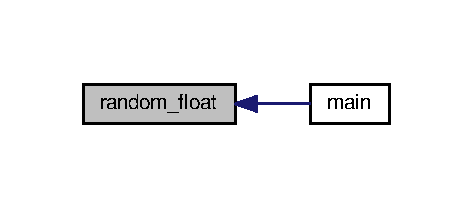
\includegraphics[width=227pt]{src_2boid_8cpp_a9594488b515ced509126c685b05f880f_icgraph}
\end{center}
\end{figure}



\hypertarget{_parametric_2_starling-_simulation_2src_2main_8cpp}{}\section{Parametric/\+Starling-\/\+Simulation/src/main.cpp File Reference}
\label{_parametric_2_starling-_simulation_2src_2main_8cpp}\index{Parametric/\+Starling-\/\+Simulation/src/main.\+cpp@{Parametric/\+Starling-\/\+Simulation/src/main.\+cpp}}
{\ttfamily \#include $<$G\+L/gl.\+h$>$}\\*
{\ttfamily \#include $<$G\+L/glu.\+h$>$}\\*
{\ttfamily \#include $<$G\+L/glut.\+h$>$}\\*
{\ttfamily \#include \char`\"{}../include/boid.\+h\char`\"{}}\\*
{\ttfamily \#include \char`\"{}../include/properties.\+h\char`\"{}}\\*
{\ttfamily \#include $<$bits/stdc++.\+h$>$}\\*
Include dependency graph for main.\+cpp\+:
\nopagebreak
\begin{figure}[H]
\begin{center}
\leavevmode
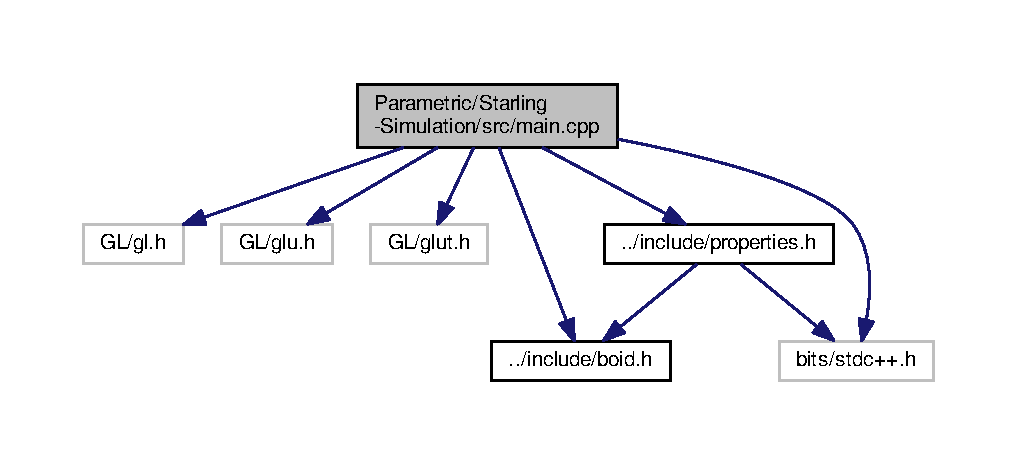
\includegraphics[width=350pt]{_parametric_2_starling-_simulation_2src_2main_8cpp__incl}
\end{center}
\end{figure}
\subsection*{Functions}
\begin{DoxyCompactItemize}
\item 
std\+::vector$<$ \hyperlink{classboid}{boid} $>$ \hyperlink{_parametric_2_starling-_simulation_2src_2main_8cpp_a3acab400bf3b180630e37bb94c8ca2d2}{v} (100)
\item 
void \hyperlink{_parametric_2_starling-_simulation_2src_2main_8cpp_a55d7e9aa910e339fa9eb7738680da6f5}{draw\+Coordinates} ()
\item 
void \hyperlink{_parametric_2_starling-_simulation_2src_2main_8cpp_a4ea013001a5fb47853d0fab8f8de35cd}{display} (void)
\item 
void \hyperlink{_parametric_2_starling-_simulation_2src_2main_8cpp_ae5474f3b746ffe82a9ec7693554a5258}{keyboard\+\_\+action} (unsigned char key, int x, int y)
\item 
void \hyperlink{_parametric_2_starling-_simulation_2src_2main_8cpp_a636e30ede2e55a392966309502eccc56}{special\+Key\+\_\+action} (int key, int x, int y)
\item 
void \hyperlink{_parametric_2_starling-_simulation_2src_2main_8cpp_a6819355374dd277347abd7c4235f0cd7}{reshape} (int width, int height)
\item 
void \hyperlink{_parametric_2_starling-_simulation_2src_2main_8cpp_a02fd73d861ef2e4aabb38c0c9ff82947}{init} ()
\item 
void \hyperlink{_parametric_2_starling-_simulation_2src_2main_8cpp_a31dc0f9d2e8cd7c620bacd665dc49d46}{go} (int a)
\item 
int \hyperlink{_parametric_2_starling-_simulation_2src_2main_8cpp_a3c04138a5bfe5d72780bb7e82a18e627}{main} (int argc, char $\ast$$\ast$argv)
\end{DoxyCompactItemize}
\subsection*{Variables}
\begin{DoxyCompactItemize}
\item 
int \hyperlink{_parametric_2_starling-_simulation_2src_2main_8cpp_ad9c7d34825651b28bdc55791ccfcf181}{rotx} =0
\item 
int \hyperlink{_parametric_2_starling-_simulation_2src_2main_8cpp_ab2fea5bf4c66da361835e03607870663}{roty} =0
\item 
int \hyperlink{_parametric_2_starling-_simulation_2src_2main_8cpp_aa47685950c49cd1ee518f5581367e231}{rotz} =0
\item 
float \hyperlink{_parametric_2_starling-_simulation_2src_2main_8cpp_a15b95adbbd613e2d9fde8dbebe324811}{transx} = 0
\item 
float \hyperlink{_parametric_2_starling-_simulation_2src_2main_8cpp_a9903321d40b0ea39b3eb992b0ef716ee}{transy} = 0
\item 
float \hyperlink{_parametric_2_starling-_simulation_2src_2main_8cpp_af3eff2bceab47fbaf2707aba16c9355b}{transz} = 0
\item 
float \hyperlink{_parametric_2_starling-_simulation_2src_2main_8cpp_a1d28dec57cce925ad92342891bd71e7c}{scale} = 0.\+001
\item 
int \hyperlink{_parametric_2_starling-_simulation_2src_2main_8cpp_aac374e320caaadeca4874add33b62af2}{w} =1000
\item 
int \hyperlink{_parametric_2_starling-_simulation_2src_2main_8cpp_a16611451551e3d15916bae723c3f59f7}{h} =1000
\item 
int \hyperlink{_parametric_2_starling-_simulation_2src_2main_8cpp_aff6586d08509fda8099d68aa8b4ae891}{ta} = 0
\item 
int \hyperlink{_parametric_2_starling-_simulation_2src_2main_8cpp_a15c345fe9f305bd944060d6a5820ab55}{qw} = 0
\end{DoxyCompactItemize}


\subsection{Function Documentation}
\index{Parametric/\+Starling-\/\+Simulation/src/main.\+cpp@{Parametric/\+Starling-\/\+Simulation/src/main.\+cpp}!display@{display}}
\index{display@{display}!Parametric/\+Starling-\/\+Simulation/src/main.\+cpp@{Parametric/\+Starling-\/\+Simulation/src/main.\+cpp}}
\subsubsection[{\texorpdfstring{display(void)}{display(void)}}]{\setlength{\rightskip}{0pt plus 5cm}void display (
\begin{DoxyParamCaption}
\item[{void}]{}
\end{DoxyParamCaption}
)}\hypertarget{_parametric_2_starling-_simulation_2src_2main_8cpp_a4ea013001a5fb47853d0fab8f8de35cd}{}\label{_parametric_2_starling-_simulation_2src_2main_8cpp_a4ea013001a5fb47853d0fab8f8de35cd}


Definition at line 68 of file main.\+cpp.



Here is the call graph for this function\+:
\nopagebreak
\begin{figure}[H]
\begin{center}
\leavevmode
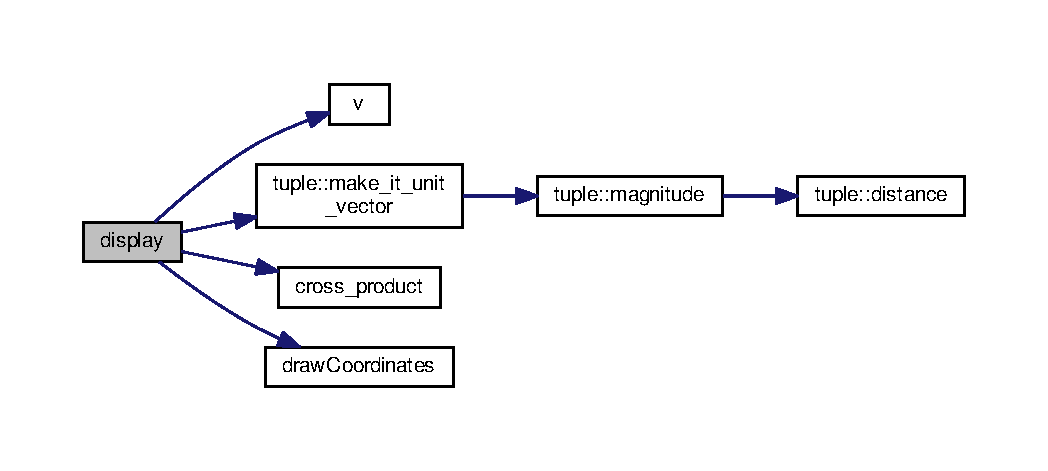
\includegraphics[width=350pt]{_parametric_2_starling-_simulation_2src_2main_8cpp_a4ea013001a5fb47853d0fab8f8de35cd_cgraph}
\end{center}
\end{figure}




Here is the caller graph for this function\+:
\nopagebreak
\begin{figure}[H]
\begin{center}
\leavevmode
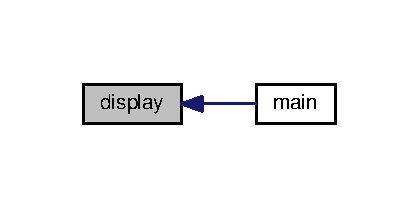
\includegraphics[width=201pt]{_parametric_2_starling-_simulation_2src_2main_8cpp_a4ea013001a5fb47853d0fab8f8de35cd_icgraph}
\end{center}
\end{figure}


\index{Parametric/\+Starling-\/\+Simulation/src/main.\+cpp@{Parametric/\+Starling-\/\+Simulation/src/main.\+cpp}!draw\+Coordinates@{draw\+Coordinates}}
\index{draw\+Coordinates@{draw\+Coordinates}!Parametric/\+Starling-\/\+Simulation/src/main.\+cpp@{Parametric/\+Starling-\/\+Simulation/src/main.\+cpp}}
\subsubsection[{\texorpdfstring{draw\+Coordinates()}{drawCoordinates()}}]{\setlength{\rightskip}{0pt plus 5cm}void draw\+Coordinates (
\begin{DoxyParamCaption}
{}
\end{DoxyParamCaption}
)}\hypertarget{_parametric_2_starling-_simulation_2src_2main_8cpp_a55d7e9aa910e339fa9eb7738680da6f5}{}\label{_parametric_2_starling-_simulation_2src_2main_8cpp_a55d7e9aa910e339fa9eb7738680da6f5}


Definition at line 17 of file main.\+cpp.



Here is the caller graph for this function\+:
\nopagebreak
\begin{figure}[H]
\begin{center}
\leavevmode
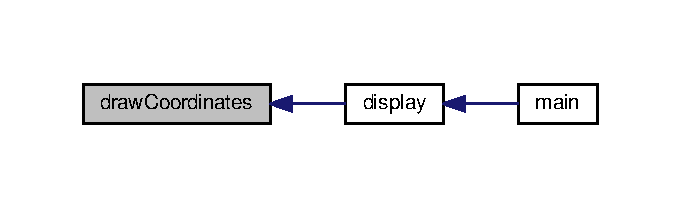
\includegraphics[width=327pt]{_parametric_2_starling-_simulation_2src_2main_8cpp_a55d7e9aa910e339fa9eb7738680da6f5_icgraph}
\end{center}
\end{figure}


\index{Parametric/\+Starling-\/\+Simulation/src/main.\+cpp@{Parametric/\+Starling-\/\+Simulation/src/main.\+cpp}!go@{go}}
\index{go@{go}!Parametric/\+Starling-\/\+Simulation/src/main.\+cpp@{Parametric/\+Starling-\/\+Simulation/src/main.\+cpp}}
\subsubsection[{\texorpdfstring{go(int a)}{go(int a)}}]{\setlength{\rightskip}{0pt plus 5cm}void go (
\begin{DoxyParamCaption}
\item[{int}]{a}
\end{DoxyParamCaption}
)}\hypertarget{_parametric_2_starling-_simulation_2src_2main_8cpp_a31dc0f9d2e8cd7c620bacd665dc49d46}{}\label{_parametric_2_starling-_simulation_2src_2main_8cpp_a31dc0f9d2e8cd7c620bacd665dc49d46}


Definition at line 286 of file main.\+cpp.



Here is the call graph for this function\+:
\nopagebreak
\begin{figure}[H]
\begin{center}
\leavevmode
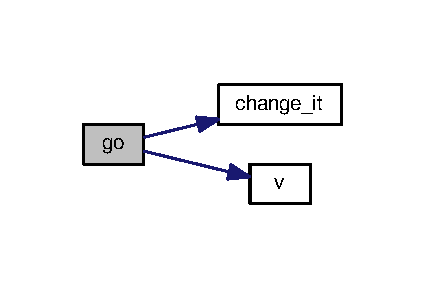
\includegraphics[width=204pt]{_parametric_2_starling-_simulation_2src_2main_8cpp_a31dc0f9d2e8cd7c620bacd665dc49d46_cgraph}
\end{center}
\end{figure}




Here is the caller graph for this function\+:
\nopagebreak
\begin{figure}[H]
\begin{center}
\leavevmode
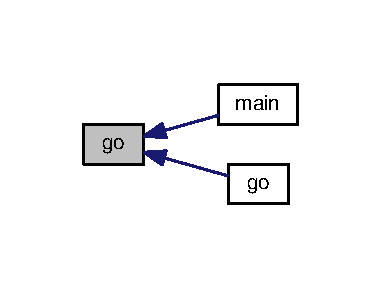
\includegraphics[width=183pt]{_parametric_2_starling-_simulation_2src_2main_8cpp_a31dc0f9d2e8cd7c620bacd665dc49d46_icgraph}
\end{center}
\end{figure}


\index{Parametric/\+Starling-\/\+Simulation/src/main.\+cpp@{Parametric/\+Starling-\/\+Simulation/src/main.\+cpp}!init@{init}}
\index{init@{init}!Parametric/\+Starling-\/\+Simulation/src/main.\+cpp@{Parametric/\+Starling-\/\+Simulation/src/main.\+cpp}}
\subsubsection[{\texorpdfstring{init()}{init()}}]{\setlength{\rightskip}{0pt plus 5cm}void init (
\begin{DoxyParamCaption}
\item[{void}]{}
\end{DoxyParamCaption}
)}\hypertarget{_parametric_2_starling-_simulation_2src_2main_8cpp_a02fd73d861ef2e4aabb38c0c9ff82947}{}\label{_parametric_2_starling-_simulation_2src_2main_8cpp_a02fd73d861ef2e4aabb38c0c9ff82947}


Definition at line 265 of file main.\+cpp.



Here is the caller graph for this function\+:
\nopagebreak
\begin{figure}[H]
\begin{center}
\leavevmode
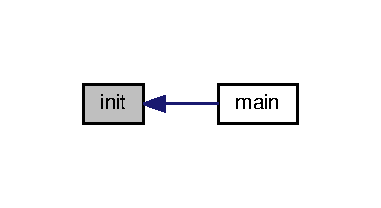
\includegraphics[width=183pt]{_parametric_2_starling-_simulation_2src_2main_8cpp_a02fd73d861ef2e4aabb38c0c9ff82947_icgraph}
\end{center}
\end{figure}


\index{Parametric/\+Starling-\/\+Simulation/src/main.\+cpp@{Parametric/\+Starling-\/\+Simulation/src/main.\+cpp}!keyboard\+\_\+action@{keyboard\+\_\+action}}
\index{keyboard\+\_\+action@{keyboard\+\_\+action}!Parametric/\+Starling-\/\+Simulation/src/main.\+cpp@{Parametric/\+Starling-\/\+Simulation/src/main.\+cpp}}
\subsubsection[{\texorpdfstring{keyboard\+\_\+action(unsigned char key, int x, int y)}{keyboard_action(unsigned char key, int x, int y)}}]{\setlength{\rightskip}{0pt plus 5cm}void keyboard\+\_\+action (
\begin{DoxyParamCaption}
\item[{unsigned char}]{key, }
\item[{int}]{x, }
\item[{int}]{y}
\end{DoxyParamCaption}
)}\hypertarget{_parametric_2_starling-_simulation_2src_2main_8cpp_ae5474f3b746ffe82a9ec7693554a5258}{}\label{_parametric_2_starling-_simulation_2src_2main_8cpp_ae5474f3b746ffe82a9ec7693554a5258}


Definition at line 178 of file main.\+cpp.



Here is the caller graph for this function\+:
\nopagebreak
\begin{figure}[H]
\begin{center}
\leavevmode
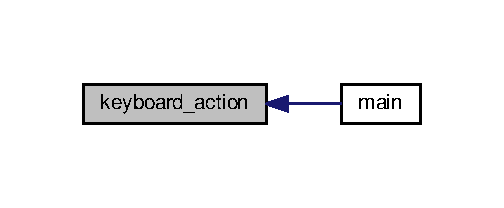
\includegraphics[width=242pt]{_parametric_2_starling-_simulation_2src_2main_8cpp_ae5474f3b746ffe82a9ec7693554a5258_icgraph}
\end{center}
\end{figure}


\index{Parametric/\+Starling-\/\+Simulation/src/main.\+cpp@{Parametric/\+Starling-\/\+Simulation/src/main.\+cpp}!main@{main}}
\index{main@{main}!Parametric/\+Starling-\/\+Simulation/src/main.\+cpp@{Parametric/\+Starling-\/\+Simulation/src/main.\+cpp}}
\subsubsection[{\texorpdfstring{main(int argc, char $\ast$$\ast$argv)}{main(int argc, char **argv)}}]{\setlength{\rightskip}{0pt plus 5cm}int main (
\begin{DoxyParamCaption}
\item[{int}]{argc, }
\item[{char $\ast$$\ast$}]{argv}
\end{DoxyParamCaption}
)}\hypertarget{_parametric_2_starling-_simulation_2src_2main_8cpp_a3c04138a5bfe5d72780bb7e82a18e627}{}\label{_parametric_2_starling-_simulation_2src_2main_8cpp_a3c04138a5bfe5d72780bb7e82a18e627}


Definition at line 293 of file main.\+cpp.



Here is the call graph for this function\+:
\nopagebreak
\begin{figure}[H]
\begin{center}
\leavevmode
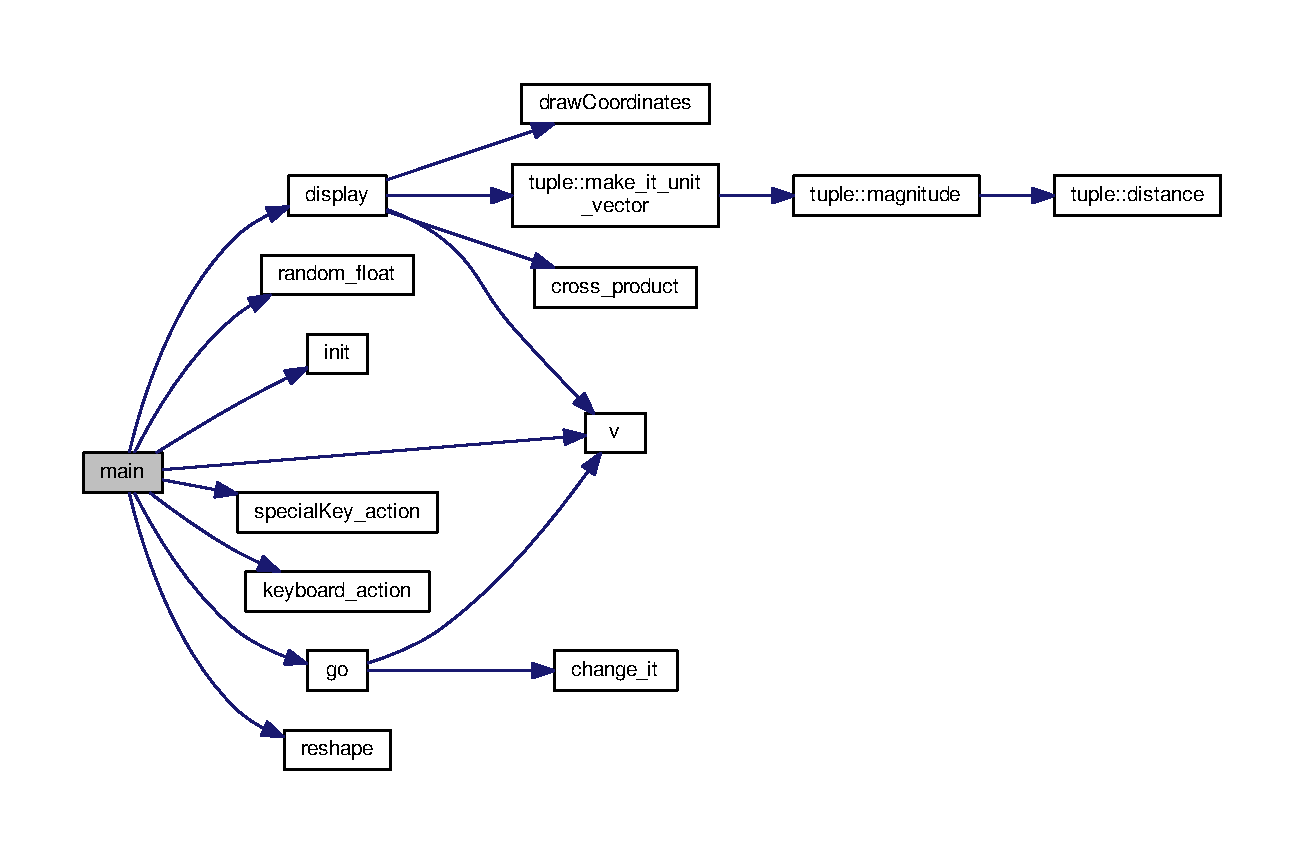
\includegraphics[width=350pt]{_parametric_2_starling-_simulation_2src_2main_8cpp_a3c04138a5bfe5d72780bb7e82a18e627_cgraph}
\end{center}
\end{figure}


\index{Parametric/\+Starling-\/\+Simulation/src/main.\+cpp@{Parametric/\+Starling-\/\+Simulation/src/main.\+cpp}!reshape@{reshape}}
\index{reshape@{reshape}!Parametric/\+Starling-\/\+Simulation/src/main.\+cpp@{Parametric/\+Starling-\/\+Simulation/src/main.\+cpp}}
\subsubsection[{\texorpdfstring{reshape(int width, int height)}{reshape(int width, int height)}}]{\setlength{\rightskip}{0pt plus 5cm}void reshape (
\begin{DoxyParamCaption}
\item[{int}]{width, }
\item[{int}]{height}
\end{DoxyParamCaption}
)}\hypertarget{_parametric_2_starling-_simulation_2src_2main_8cpp_a6819355374dd277347abd7c4235f0cd7}{}\label{_parametric_2_starling-_simulation_2src_2main_8cpp_a6819355374dd277347abd7c4235f0cd7}


Definition at line 246 of file main.\+cpp.



Here is the caller graph for this function\+:
\nopagebreak
\begin{figure}[H]
\begin{center}
\leavevmode
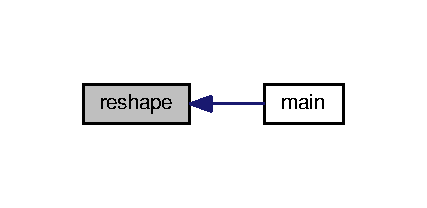
\includegraphics[width=205pt]{_parametric_2_starling-_simulation_2src_2main_8cpp_a6819355374dd277347abd7c4235f0cd7_icgraph}
\end{center}
\end{figure}


\index{Parametric/\+Starling-\/\+Simulation/src/main.\+cpp@{Parametric/\+Starling-\/\+Simulation/src/main.\+cpp}!special\+Key\+\_\+action@{special\+Key\+\_\+action}}
\index{special\+Key\+\_\+action@{special\+Key\+\_\+action}!Parametric/\+Starling-\/\+Simulation/src/main.\+cpp@{Parametric/\+Starling-\/\+Simulation/src/main.\+cpp}}
\subsubsection[{\texorpdfstring{special\+Key\+\_\+action(int key, int x, int y)}{specialKey_action(int key, int x, int y)}}]{\setlength{\rightskip}{0pt plus 5cm}void special\+Key\+\_\+action (
\begin{DoxyParamCaption}
\item[{int}]{key, }
\item[{int}]{x, }
\item[{int}]{y}
\end{DoxyParamCaption}
)}\hypertarget{_parametric_2_starling-_simulation_2src_2main_8cpp_a636e30ede2e55a392966309502eccc56}{}\label{_parametric_2_starling-_simulation_2src_2main_8cpp_a636e30ede2e55a392966309502eccc56}


Definition at line 231 of file main.\+cpp.



Here is the caller graph for this function\+:
\nopagebreak
\begin{figure}[H]
\begin{center}
\leavevmode
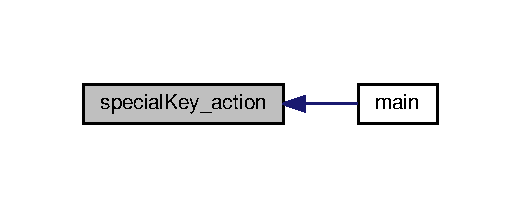
\includegraphics[width=250pt]{_parametric_2_starling-_simulation_2src_2main_8cpp_a636e30ede2e55a392966309502eccc56_icgraph}
\end{center}
\end{figure}


\index{Parametric/\+Starling-\/\+Simulation/src/main.\+cpp@{Parametric/\+Starling-\/\+Simulation/src/main.\+cpp}!v@{v}}
\index{v@{v}!Parametric/\+Starling-\/\+Simulation/src/main.\+cpp@{Parametric/\+Starling-\/\+Simulation/src/main.\+cpp}}
\subsubsection[{\texorpdfstring{v(100)}{v(100)}}]{\setlength{\rightskip}{0pt plus 5cm}std\+::vector$<${\bf boid}$>$ v (
\begin{DoxyParamCaption}
\item[{100}]{}
\end{DoxyParamCaption}
)}\hypertarget{_parametric_2_starling-_simulation_2src_2main_8cpp_a3acab400bf3b180630e37bb94c8ca2d2}{}\label{_parametric_2_starling-_simulation_2src_2main_8cpp_a3acab400bf3b180630e37bb94c8ca2d2}


Here is the caller graph for this function\+:
\nopagebreak
\begin{figure}[H]
\begin{center}
\leavevmode
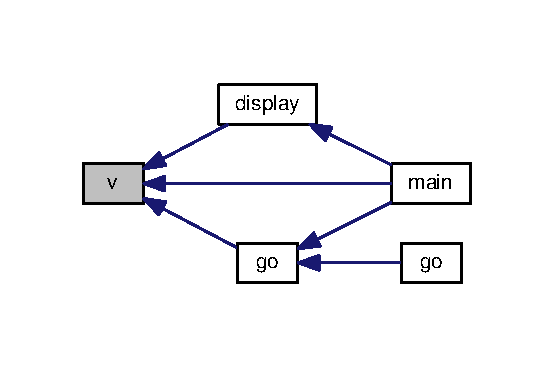
\includegraphics[width=266pt]{_parametric_2_starling-_simulation_2src_2main_8cpp_a3acab400bf3b180630e37bb94c8ca2d2_icgraph}
\end{center}
\end{figure}




\subsection{Variable Documentation}
\index{Parametric/\+Starling-\/\+Simulation/src/main.\+cpp@{Parametric/\+Starling-\/\+Simulation/src/main.\+cpp}!h@{h}}
\index{h@{h}!Parametric/\+Starling-\/\+Simulation/src/main.\+cpp@{Parametric/\+Starling-\/\+Simulation/src/main.\+cpp}}
\subsubsection[{\texorpdfstring{h}{h}}]{\setlength{\rightskip}{0pt plus 5cm}int h =1000}\hypertarget{_parametric_2_starling-_simulation_2src_2main_8cpp_a16611451551e3d15916bae723c3f59f7}{}\label{_parametric_2_starling-_simulation_2src_2main_8cpp_a16611451551e3d15916bae723c3f59f7}


Definition at line 11 of file main.\+cpp.

\index{Parametric/\+Starling-\/\+Simulation/src/main.\+cpp@{Parametric/\+Starling-\/\+Simulation/src/main.\+cpp}!qw@{qw}}
\index{qw@{qw}!Parametric/\+Starling-\/\+Simulation/src/main.\+cpp@{Parametric/\+Starling-\/\+Simulation/src/main.\+cpp}}
\subsubsection[{\texorpdfstring{qw}{qw}}]{\setlength{\rightskip}{0pt plus 5cm}int qw = 0}\hypertarget{_parametric_2_starling-_simulation_2src_2main_8cpp_a15c345fe9f305bd944060d6a5820ab55}{}\label{_parametric_2_starling-_simulation_2src_2main_8cpp_a15c345fe9f305bd944060d6a5820ab55}


Definition at line 13 of file main.\+cpp.

\index{Parametric/\+Starling-\/\+Simulation/src/main.\+cpp@{Parametric/\+Starling-\/\+Simulation/src/main.\+cpp}!rotx@{rotx}}
\index{rotx@{rotx}!Parametric/\+Starling-\/\+Simulation/src/main.\+cpp@{Parametric/\+Starling-\/\+Simulation/src/main.\+cpp}}
\subsubsection[{\texorpdfstring{rotx}{rotx}}]{\setlength{\rightskip}{0pt plus 5cm}int rotx =0}\hypertarget{_parametric_2_starling-_simulation_2src_2main_8cpp_ad9c7d34825651b28bdc55791ccfcf181}{}\label{_parametric_2_starling-_simulation_2src_2main_8cpp_ad9c7d34825651b28bdc55791ccfcf181}


Definition at line 9 of file main.\+cpp.

\index{Parametric/\+Starling-\/\+Simulation/src/main.\+cpp@{Parametric/\+Starling-\/\+Simulation/src/main.\+cpp}!roty@{roty}}
\index{roty@{roty}!Parametric/\+Starling-\/\+Simulation/src/main.\+cpp@{Parametric/\+Starling-\/\+Simulation/src/main.\+cpp}}
\subsubsection[{\texorpdfstring{roty}{roty}}]{\setlength{\rightskip}{0pt plus 5cm}int roty =0}\hypertarget{_parametric_2_starling-_simulation_2src_2main_8cpp_ab2fea5bf4c66da361835e03607870663}{}\label{_parametric_2_starling-_simulation_2src_2main_8cpp_ab2fea5bf4c66da361835e03607870663}


Definition at line 9 of file main.\+cpp.

\index{Parametric/\+Starling-\/\+Simulation/src/main.\+cpp@{Parametric/\+Starling-\/\+Simulation/src/main.\+cpp}!rotz@{rotz}}
\index{rotz@{rotz}!Parametric/\+Starling-\/\+Simulation/src/main.\+cpp@{Parametric/\+Starling-\/\+Simulation/src/main.\+cpp}}
\subsubsection[{\texorpdfstring{rotz}{rotz}}]{\setlength{\rightskip}{0pt plus 5cm}int rotz =0}\hypertarget{_parametric_2_starling-_simulation_2src_2main_8cpp_aa47685950c49cd1ee518f5581367e231}{}\label{_parametric_2_starling-_simulation_2src_2main_8cpp_aa47685950c49cd1ee518f5581367e231}


Definition at line 9 of file main.\+cpp.

\index{Parametric/\+Starling-\/\+Simulation/src/main.\+cpp@{Parametric/\+Starling-\/\+Simulation/src/main.\+cpp}!scale@{scale}}
\index{scale@{scale}!Parametric/\+Starling-\/\+Simulation/src/main.\+cpp@{Parametric/\+Starling-\/\+Simulation/src/main.\+cpp}}
\subsubsection[{\texorpdfstring{scale}{scale}}]{\setlength{\rightskip}{0pt plus 5cm}float scale = 0.\+001}\hypertarget{_parametric_2_starling-_simulation_2src_2main_8cpp_a1d28dec57cce925ad92342891bd71e7c}{}\label{_parametric_2_starling-_simulation_2src_2main_8cpp_a1d28dec57cce925ad92342891bd71e7c}


Definition at line 10 of file main.\+cpp.

\index{Parametric/\+Starling-\/\+Simulation/src/main.\+cpp@{Parametric/\+Starling-\/\+Simulation/src/main.\+cpp}!ta@{ta}}
\index{ta@{ta}!Parametric/\+Starling-\/\+Simulation/src/main.\+cpp@{Parametric/\+Starling-\/\+Simulation/src/main.\+cpp}}
\subsubsection[{\texorpdfstring{ta}{ta}}]{\setlength{\rightskip}{0pt plus 5cm}int ta = 0}\hypertarget{_parametric_2_starling-_simulation_2src_2main_8cpp_aff6586d08509fda8099d68aa8b4ae891}{}\label{_parametric_2_starling-_simulation_2src_2main_8cpp_aff6586d08509fda8099d68aa8b4ae891}


Definition at line 12 of file main.\+cpp.

\index{Parametric/\+Starling-\/\+Simulation/src/main.\+cpp@{Parametric/\+Starling-\/\+Simulation/src/main.\+cpp}!transx@{transx}}
\index{transx@{transx}!Parametric/\+Starling-\/\+Simulation/src/main.\+cpp@{Parametric/\+Starling-\/\+Simulation/src/main.\+cpp}}
\subsubsection[{\texorpdfstring{transx}{transx}}]{\setlength{\rightskip}{0pt plus 5cm}float transx = 0}\hypertarget{_parametric_2_starling-_simulation_2src_2main_8cpp_a15b95adbbd613e2d9fde8dbebe324811}{}\label{_parametric_2_starling-_simulation_2src_2main_8cpp_a15b95adbbd613e2d9fde8dbebe324811}


Definition at line 10 of file main.\+cpp.

\index{Parametric/\+Starling-\/\+Simulation/src/main.\+cpp@{Parametric/\+Starling-\/\+Simulation/src/main.\+cpp}!transy@{transy}}
\index{transy@{transy}!Parametric/\+Starling-\/\+Simulation/src/main.\+cpp@{Parametric/\+Starling-\/\+Simulation/src/main.\+cpp}}
\subsubsection[{\texorpdfstring{transy}{transy}}]{\setlength{\rightskip}{0pt plus 5cm}float transy = 0}\hypertarget{_parametric_2_starling-_simulation_2src_2main_8cpp_a9903321d40b0ea39b3eb992b0ef716ee}{}\label{_parametric_2_starling-_simulation_2src_2main_8cpp_a9903321d40b0ea39b3eb992b0ef716ee}


Definition at line 10 of file main.\+cpp.

\index{Parametric/\+Starling-\/\+Simulation/src/main.\+cpp@{Parametric/\+Starling-\/\+Simulation/src/main.\+cpp}!transz@{transz}}
\index{transz@{transz}!Parametric/\+Starling-\/\+Simulation/src/main.\+cpp@{Parametric/\+Starling-\/\+Simulation/src/main.\+cpp}}
\subsubsection[{\texorpdfstring{transz}{transz}}]{\setlength{\rightskip}{0pt plus 5cm}float transz = 0}\hypertarget{_parametric_2_starling-_simulation_2src_2main_8cpp_af3eff2bceab47fbaf2707aba16c9355b}{}\label{_parametric_2_starling-_simulation_2src_2main_8cpp_af3eff2bceab47fbaf2707aba16c9355b}


Definition at line 10 of file main.\+cpp.

\index{Parametric/\+Starling-\/\+Simulation/src/main.\+cpp@{Parametric/\+Starling-\/\+Simulation/src/main.\+cpp}!w@{w}}
\index{w@{w}!Parametric/\+Starling-\/\+Simulation/src/main.\+cpp@{Parametric/\+Starling-\/\+Simulation/src/main.\+cpp}}
\subsubsection[{\texorpdfstring{w}{w}}]{\setlength{\rightskip}{0pt plus 5cm}int w =1000}\hypertarget{_parametric_2_starling-_simulation_2src_2main_8cpp_aac374e320caaadeca4874add33b62af2}{}\label{_parametric_2_starling-_simulation_2src_2main_8cpp_aac374e320caaadeca4874add33b62af2}


Definition at line 11 of file main.\+cpp.


\hypertarget{src_2main_8cpp}{}\section{src/main.cpp File Reference}
\label{src_2main_8cpp}\index{src/main.\+cpp@{src/main.\+cpp}}
{\ttfamily \#include $<$G\+L/gl.\+h$>$}\\*
{\ttfamily \#include $<$G\+L/glu.\+h$>$}\\*
{\ttfamily \#include $<$G\+L/glut.\+h$>$}\\*
{\ttfamily \#include \char`\"{}../include/boid.\+h\char`\"{}}\\*
{\ttfamily \#include \char`\"{}../include/properties.\+h\char`\"{}}\\*
{\ttfamily \#include $<$bits/stdc++.\+h$>$}\\*
Include dependency graph for main.\+cpp\+:
\nopagebreak
\begin{figure}[H]
\begin{center}
\leavevmode
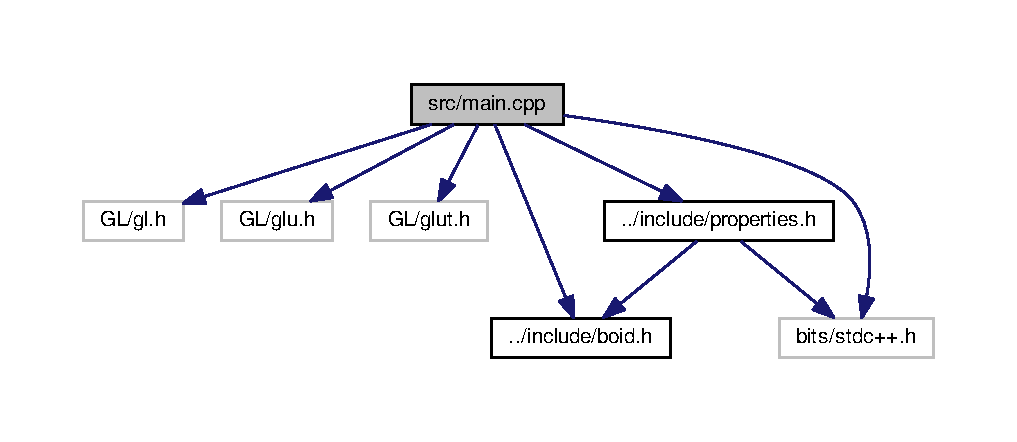
\includegraphics[width=350pt]{src_2main_8cpp__incl}
\end{center}
\end{figure}
\subsection*{Functions}
\begin{DoxyCompactItemize}
\item 
std\+::vector$<$ \hyperlink{classboid}{boid} $>$ \hyperlink{src_2main_8cpp_a1d5a718f1d6b42141bc3a6834be5e420}{v} (20)
\item 
void \hyperlink{src_2main_8cpp_a55d7e9aa910e339fa9eb7738680da6f5}{draw\+Coordinates} ()
\item 
void \hyperlink{src_2main_8cpp_a4ea013001a5fb47853d0fab8f8de35cd}{display} (void)
\item 
void \hyperlink{src_2main_8cpp_ae5474f3b746ffe82a9ec7693554a5258}{keyboard\+\_\+action} (unsigned char key, int x, int y)
\item 
void \hyperlink{src_2main_8cpp_a636e30ede2e55a392966309502eccc56}{special\+Key\+\_\+action} (int key, int x, int y)
\item 
void \hyperlink{src_2main_8cpp_a6819355374dd277347abd7c4235f0cd7}{reshape} (int width, int height)
\item 
void \hyperlink{src_2main_8cpp_a02fd73d861ef2e4aabb38c0c9ff82947}{init} ()
\item 
void \hyperlink{src_2main_8cpp_a31dc0f9d2e8cd7c620bacd665dc49d46}{go} (int a)
\item 
int \hyperlink{src_2main_8cpp_a3c04138a5bfe5d72780bb7e82a18e627}{main} (int argc, char $\ast$$\ast$argv)
\end{DoxyCompactItemize}
\subsection*{Variables}
\begin{DoxyCompactItemize}
\item 
int \hyperlink{src_2main_8cpp_ad9c7d34825651b28bdc55791ccfcf181}{rotx} =0
\item 
int \hyperlink{src_2main_8cpp_ab2fea5bf4c66da361835e03607870663}{roty} =0
\item 
int \hyperlink{src_2main_8cpp_aa47685950c49cd1ee518f5581367e231}{rotz} =0
\item 
float \hyperlink{src_2main_8cpp_a15b95adbbd613e2d9fde8dbebe324811}{transx} = 0
\item 
float \hyperlink{src_2main_8cpp_a9903321d40b0ea39b3eb992b0ef716ee}{transy} = 0
\item 
float \hyperlink{src_2main_8cpp_af3eff2bceab47fbaf2707aba16c9355b}{transz} = 0
\item 
float \hyperlink{src_2main_8cpp_a1d28dec57cce925ad92342891bd71e7c}{scale} = 0.\+001
\item 
int \hyperlink{src_2main_8cpp_aac374e320caaadeca4874add33b62af2}{w} =1000
\item 
int \hyperlink{src_2main_8cpp_a16611451551e3d15916bae723c3f59f7}{h} =1000
\item 
int \hyperlink{src_2main_8cpp_aff6586d08509fda8099d68aa8b4ae891}{ta} = 0
\item 
int \hyperlink{src_2main_8cpp_a15c345fe9f305bd944060d6a5820ab55}{qw} = 0
\end{DoxyCompactItemize}


\subsection{Function Documentation}
\index{src/main.\+cpp@{src/main.\+cpp}!display@{display}}
\index{display@{display}!src/main.\+cpp@{src/main.\+cpp}}
\subsubsection[{\texorpdfstring{display(void)}{display(void)}}]{\setlength{\rightskip}{0pt plus 5cm}void display (
\begin{DoxyParamCaption}
\item[{void}]{}
\end{DoxyParamCaption}
)}\hypertarget{src_2main_8cpp_a4ea013001a5fb47853d0fab8f8de35cd}{}\label{src_2main_8cpp_a4ea013001a5fb47853d0fab8f8de35cd}


Definition at line 68 of file main.\+cpp.



Here is the call graph for this function\+:
\nopagebreak
\begin{figure}[H]
\begin{center}
\leavevmode
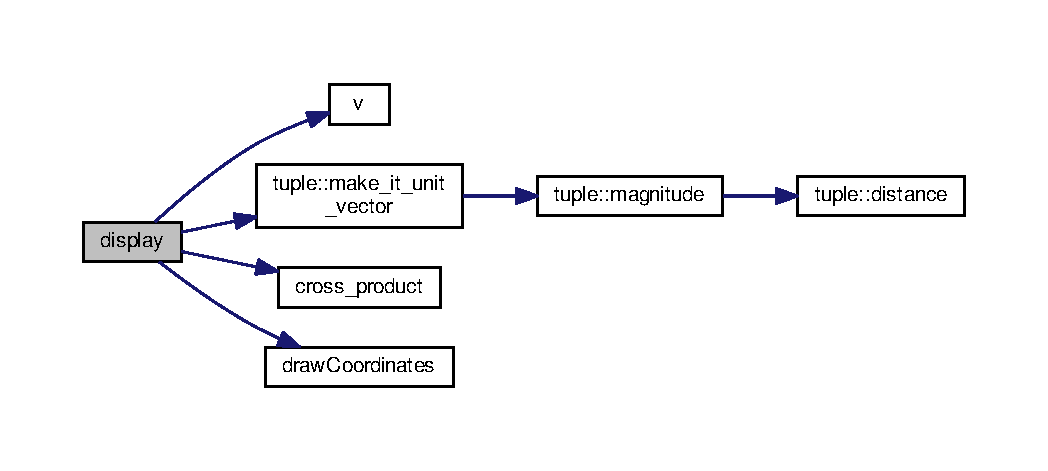
\includegraphics[width=350pt]{src_2main_8cpp_a4ea013001a5fb47853d0fab8f8de35cd_cgraph}
\end{center}
\end{figure}


\index{src/main.\+cpp@{src/main.\+cpp}!draw\+Coordinates@{draw\+Coordinates}}
\index{draw\+Coordinates@{draw\+Coordinates}!src/main.\+cpp@{src/main.\+cpp}}
\subsubsection[{\texorpdfstring{draw\+Coordinates()}{drawCoordinates()}}]{\setlength{\rightskip}{0pt plus 5cm}void draw\+Coordinates (
\begin{DoxyParamCaption}
{}
\end{DoxyParamCaption}
)}\hypertarget{src_2main_8cpp_a55d7e9aa910e339fa9eb7738680da6f5}{}\label{src_2main_8cpp_a55d7e9aa910e339fa9eb7738680da6f5}


Definition at line 17 of file main.\+cpp.

\index{src/main.\+cpp@{src/main.\+cpp}!go@{go}}
\index{go@{go}!src/main.\+cpp@{src/main.\+cpp}}
\subsubsection[{\texorpdfstring{go(int a)}{go(int a)}}]{\setlength{\rightskip}{0pt plus 5cm}void go (
\begin{DoxyParamCaption}
\item[{int}]{a}
\end{DoxyParamCaption}
)}\hypertarget{src_2main_8cpp_a31dc0f9d2e8cd7c620bacd665dc49d46}{}\label{src_2main_8cpp_a31dc0f9d2e8cd7c620bacd665dc49d46}


Definition at line 279 of file main.\+cpp.



Here is the call graph for this function\+:
\nopagebreak
\begin{figure}[H]
\begin{center}
\leavevmode
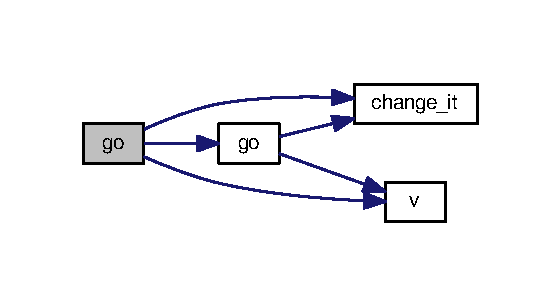
\includegraphics[width=269pt]{src_2main_8cpp_a31dc0f9d2e8cd7c620bacd665dc49d46_cgraph}
\end{center}
\end{figure}


\index{src/main.\+cpp@{src/main.\+cpp}!init@{init}}
\index{init@{init}!src/main.\+cpp@{src/main.\+cpp}}
\subsubsection[{\texorpdfstring{init()}{init()}}]{\setlength{\rightskip}{0pt plus 5cm}void init (
\begin{DoxyParamCaption}
\item[{void}]{}
\end{DoxyParamCaption}
)}\hypertarget{src_2main_8cpp_a02fd73d861ef2e4aabb38c0c9ff82947}{}\label{src_2main_8cpp_a02fd73d861ef2e4aabb38c0c9ff82947}


Definition at line 258 of file main.\+cpp.

\index{src/main.\+cpp@{src/main.\+cpp}!keyboard\+\_\+action@{keyboard\+\_\+action}}
\index{keyboard\+\_\+action@{keyboard\+\_\+action}!src/main.\+cpp@{src/main.\+cpp}}
\subsubsection[{\texorpdfstring{keyboard\+\_\+action(unsigned char key, int x, int y)}{keyboard_action(unsigned char key, int x, int y)}}]{\setlength{\rightskip}{0pt plus 5cm}void keyboard\+\_\+action (
\begin{DoxyParamCaption}
\item[{unsigned char}]{key, }
\item[{int}]{x, }
\item[{int}]{y}
\end{DoxyParamCaption}
)}\hypertarget{src_2main_8cpp_ae5474f3b746ffe82a9ec7693554a5258}{}\label{src_2main_8cpp_ae5474f3b746ffe82a9ec7693554a5258}


Definition at line 171 of file main.\+cpp.

\index{src/main.\+cpp@{src/main.\+cpp}!main@{main}}
\index{main@{main}!src/main.\+cpp@{src/main.\+cpp}}
\subsubsection[{\texorpdfstring{main(int argc, char $\ast$$\ast$argv)}{main(int argc, char **argv)}}]{\setlength{\rightskip}{0pt plus 5cm}int main (
\begin{DoxyParamCaption}
\item[{int}]{argc, }
\item[{char $\ast$$\ast$}]{argv}
\end{DoxyParamCaption}
)}\hypertarget{src_2main_8cpp_a3c04138a5bfe5d72780bb7e82a18e627}{}\label{src_2main_8cpp_a3c04138a5bfe5d72780bb7e82a18e627}


Definition at line 286 of file main.\+cpp.



Here is the call graph for this function\+:
\nopagebreak
\begin{figure}[H]
\begin{center}
\leavevmode
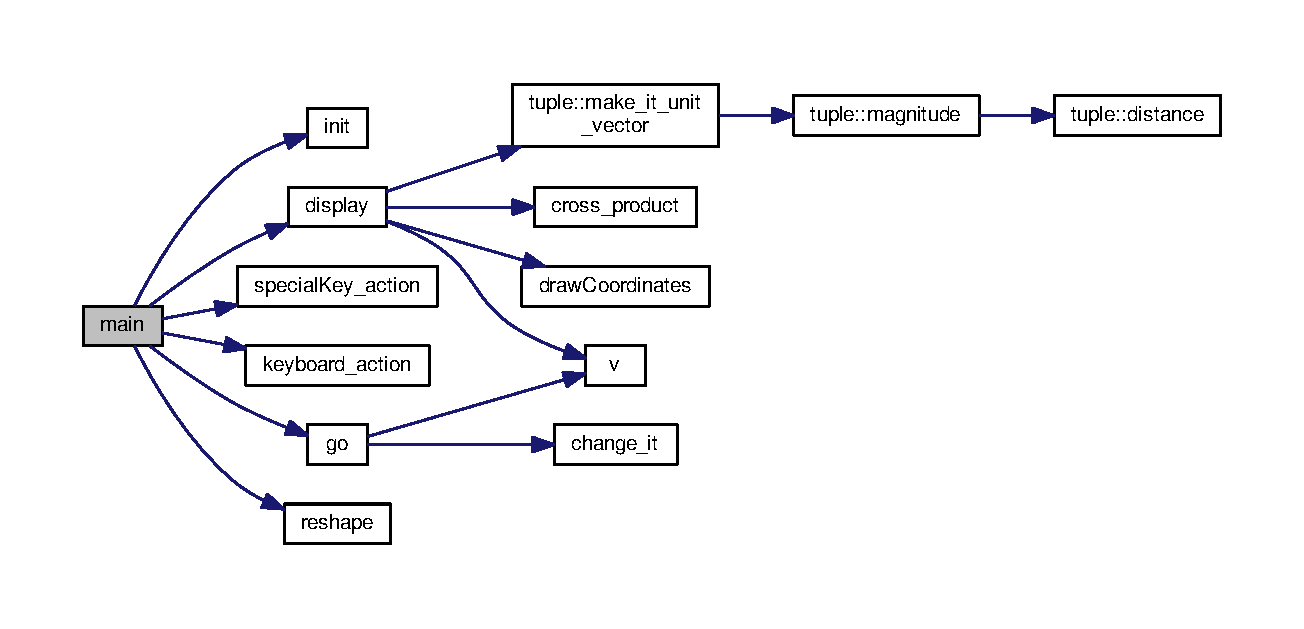
\includegraphics[width=350pt]{src_2main_8cpp_a3c04138a5bfe5d72780bb7e82a18e627_cgraph}
\end{center}
\end{figure}


\index{src/main.\+cpp@{src/main.\+cpp}!reshape@{reshape}}
\index{reshape@{reshape}!src/main.\+cpp@{src/main.\+cpp}}
\subsubsection[{\texorpdfstring{reshape(int width, int height)}{reshape(int width, int height)}}]{\setlength{\rightskip}{0pt plus 5cm}void reshape (
\begin{DoxyParamCaption}
\item[{int}]{width, }
\item[{int}]{height}
\end{DoxyParamCaption}
)}\hypertarget{src_2main_8cpp_a6819355374dd277347abd7c4235f0cd7}{}\label{src_2main_8cpp_a6819355374dd277347abd7c4235f0cd7}


Definition at line 239 of file main.\+cpp.

\index{src/main.\+cpp@{src/main.\+cpp}!special\+Key\+\_\+action@{special\+Key\+\_\+action}}
\index{special\+Key\+\_\+action@{special\+Key\+\_\+action}!src/main.\+cpp@{src/main.\+cpp}}
\subsubsection[{\texorpdfstring{special\+Key\+\_\+action(int key, int x, int y)}{specialKey_action(int key, int x, int y)}}]{\setlength{\rightskip}{0pt plus 5cm}void special\+Key\+\_\+action (
\begin{DoxyParamCaption}
\item[{int}]{key, }
\item[{int}]{x, }
\item[{int}]{y}
\end{DoxyParamCaption}
)}\hypertarget{src_2main_8cpp_a636e30ede2e55a392966309502eccc56}{}\label{src_2main_8cpp_a636e30ede2e55a392966309502eccc56}


Definition at line 224 of file main.\+cpp.

\index{src/main.\+cpp@{src/main.\+cpp}!v@{v}}
\index{v@{v}!src/main.\+cpp@{src/main.\+cpp}}
\subsubsection[{\texorpdfstring{v(20)}{v(20)}}]{\setlength{\rightskip}{0pt plus 5cm}std\+::vector$<${\bf boid}$>$ v (
\begin{DoxyParamCaption}
\item[{20}]{}
\end{DoxyParamCaption}
)}\hypertarget{src_2main_8cpp_a1d5a718f1d6b42141bc3a6834be5e420}{}\label{src_2main_8cpp_a1d5a718f1d6b42141bc3a6834be5e420}


\subsection{Variable Documentation}
\index{src/main.\+cpp@{src/main.\+cpp}!h@{h}}
\index{h@{h}!src/main.\+cpp@{src/main.\+cpp}}
\subsubsection[{\texorpdfstring{h}{h}}]{\setlength{\rightskip}{0pt plus 5cm}int h =1000}\hypertarget{src_2main_8cpp_a16611451551e3d15916bae723c3f59f7}{}\label{src_2main_8cpp_a16611451551e3d15916bae723c3f59f7}


Definition at line 11 of file main.\+cpp.

\index{src/main.\+cpp@{src/main.\+cpp}!qw@{qw}}
\index{qw@{qw}!src/main.\+cpp@{src/main.\+cpp}}
\subsubsection[{\texorpdfstring{qw}{qw}}]{\setlength{\rightskip}{0pt plus 5cm}int qw = 0}\hypertarget{src_2main_8cpp_a15c345fe9f305bd944060d6a5820ab55}{}\label{src_2main_8cpp_a15c345fe9f305bd944060d6a5820ab55}


Definition at line 13 of file main.\+cpp.

\index{src/main.\+cpp@{src/main.\+cpp}!rotx@{rotx}}
\index{rotx@{rotx}!src/main.\+cpp@{src/main.\+cpp}}
\subsubsection[{\texorpdfstring{rotx}{rotx}}]{\setlength{\rightskip}{0pt plus 5cm}int rotx =0}\hypertarget{src_2main_8cpp_ad9c7d34825651b28bdc55791ccfcf181}{}\label{src_2main_8cpp_ad9c7d34825651b28bdc55791ccfcf181}


Definition at line 9 of file main.\+cpp.

\index{src/main.\+cpp@{src/main.\+cpp}!roty@{roty}}
\index{roty@{roty}!src/main.\+cpp@{src/main.\+cpp}}
\subsubsection[{\texorpdfstring{roty}{roty}}]{\setlength{\rightskip}{0pt plus 5cm}int roty =0}\hypertarget{src_2main_8cpp_ab2fea5bf4c66da361835e03607870663}{}\label{src_2main_8cpp_ab2fea5bf4c66da361835e03607870663}


Definition at line 9 of file main.\+cpp.

\index{src/main.\+cpp@{src/main.\+cpp}!rotz@{rotz}}
\index{rotz@{rotz}!src/main.\+cpp@{src/main.\+cpp}}
\subsubsection[{\texorpdfstring{rotz}{rotz}}]{\setlength{\rightskip}{0pt plus 5cm}int rotz =0}\hypertarget{src_2main_8cpp_aa47685950c49cd1ee518f5581367e231}{}\label{src_2main_8cpp_aa47685950c49cd1ee518f5581367e231}


Definition at line 9 of file main.\+cpp.

\index{src/main.\+cpp@{src/main.\+cpp}!scale@{scale}}
\index{scale@{scale}!src/main.\+cpp@{src/main.\+cpp}}
\subsubsection[{\texorpdfstring{scale}{scale}}]{\setlength{\rightskip}{0pt plus 5cm}float scale = 0.\+001}\hypertarget{src_2main_8cpp_a1d28dec57cce925ad92342891bd71e7c}{}\label{src_2main_8cpp_a1d28dec57cce925ad92342891bd71e7c}


Definition at line 10 of file main.\+cpp.

\index{src/main.\+cpp@{src/main.\+cpp}!ta@{ta}}
\index{ta@{ta}!src/main.\+cpp@{src/main.\+cpp}}
\subsubsection[{\texorpdfstring{ta}{ta}}]{\setlength{\rightskip}{0pt plus 5cm}int ta = 0}\hypertarget{src_2main_8cpp_aff6586d08509fda8099d68aa8b4ae891}{}\label{src_2main_8cpp_aff6586d08509fda8099d68aa8b4ae891}


Definition at line 12 of file main.\+cpp.

\index{src/main.\+cpp@{src/main.\+cpp}!transx@{transx}}
\index{transx@{transx}!src/main.\+cpp@{src/main.\+cpp}}
\subsubsection[{\texorpdfstring{transx}{transx}}]{\setlength{\rightskip}{0pt plus 5cm}float transx = 0}\hypertarget{src_2main_8cpp_a15b95adbbd613e2d9fde8dbebe324811}{}\label{src_2main_8cpp_a15b95adbbd613e2d9fde8dbebe324811}


Definition at line 10 of file main.\+cpp.

\index{src/main.\+cpp@{src/main.\+cpp}!transy@{transy}}
\index{transy@{transy}!src/main.\+cpp@{src/main.\+cpp}}
\subsubsection[{\texorpdfstring{transy}{transy}}]{\setlength{\rightskip}{0pt plus 5cm}float transy = 0}\hypertarget{src_2main_8cpp_a9903321d40b0ea39b3eb992b0ef716ee}{}\label{src_2main_8cpp_a9903321d40b0ea39b3eb992b0ef716ee}


Definition at line 10 of file main.\+cpp.

\index{src/main.\+cpp@{src/main.\+cpp}!transz@{transz}}
\index{transz@{transz}!src/main.\+cpp@{src/main.\+cpp}}
\subsubsection[{\texorpdfstring{transz}{transz}}]{\setlength{\rightskip}{0pt plus 5cm}float transz = 0}\hypertarget{src_2main_8cpp_af3eff2bceab47fbaf2707aba16c9355b}{}\label{src_2main_8cpp_af3eff2bceab47fbaf2707aba16c9355b}


Definition at line 10 of file main.\+cpp.

\index{src/main.\+cpp@{src/main.\+cpp}!w@{w}}
\index{w@{w}!src/main.\+cpp@{src/main.\+cpp}}
\subsubsection[{\texorpdfstring{w}{w}}]{\setlength{\rightskip}{0pt plus 5cm}int w =1000}\hypertarget{src_2main_8cpp_aac374e320caaadeca4874add33b62af2}{}\label{src_2main_8cpp_aac374e320caaadeca4874add33b62af2}


Definition at line 11 of file main.\+cpp.


\hypertarget{_parametric_2_starling-_simulation_2src_2properties_8cpp}{}\section{Parametric/\+Starling-\/\+Simulation/src/properties.cpp File Reference}
\label{_parametric_2_starling-_simulation_2src_2properties_8cpp}\index{Parametric/\+Starling-\/\+Simulation/src/properties.\+cpp@{Parametric/\+Starling-\/\+Simulation/src/properties.\+cpp}}
{\ttfamily \#include \char`\"{}../include/properties.\+h\char`\"{}}\\*
{\ttfamily \#include $<$bits/stdc++.\+h$>$}\\*
Include dependency graph for properties.\+cpp\+:
\nopagebreak
\begin{figure}[H]
\begin{center}
\leavevmode
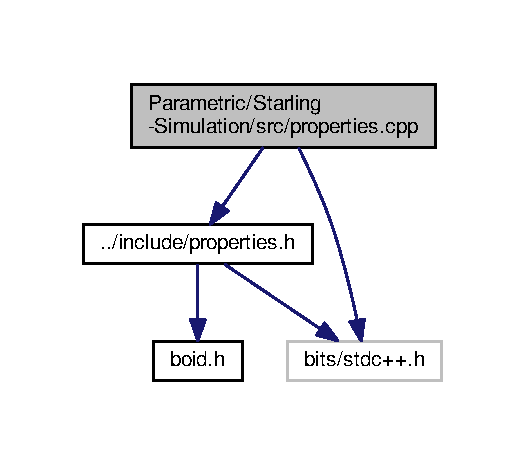
\includegraphics[width=252pt]{_parametric_2_starling-_simulation_2src_2properties_8cpp__incl}
\end{center}
\end{figure}
\subsection*{Macros}
\begin{DoxyCompactItemize}
\item 
\#define \hyperlink{_parametric_2_starling-_simulation_2src_2properties_8cpp_ab53328405fd9ba89990d9426d0e6389e}{eps}~0.\+000001
\item 
\#define \hyperlink{_parametric_2_starling-_simulation_2src_2properties_8cpp_ab16f7f055bbbd643b9510d1bd42eb4dc}{cohesion\+\_\+coeff}~3.\+0
\item 
\#define \hyperlink{_parametric_2_starling-_simulation_2src_2properties_8cpp_a7f599c3f3ac600fcccbd330b534e48ae}{separation\+\_\+coeff}~2.\+0
\item 
\#define \hyperlink{_parametric_2_starling-_simulation_2src_2properties_8cpp_a9439746dd157dbb69b93e084d1edfb01}{alignment\+\_\+coeff}~0.\+5
\item 
\#define \hyperlink{_parametric_2_starling-_simulation_2src_2properties_8cpp_aada98d3e75b15aaf71743634702209b2}{inertia\+\_\+coeff}~0.\+1
\item 
\#define \hyperlink{_parametric_2_starling-_simulation_2src_2properties_8cpp_a77da7eab1cc4cbb2c82f162c70fbc5c6}{boundary\+\_\+repulsion\+\_\+coeff}~0.\+8
\item 
\#define \hyperlink{_parametric_2_starling-_simulation_2src_2properties_8cpp_ae3ae4055677d82207f6578facdb0fc9f}{wall\+\_\+coeff}~50.\+0
\item 
\#define \hyperlink{_parametric_2_starling-_simulation_2src_2properties_8cpp_aa1f49d89b055225bac6ab75db254c1b3}{wall\+\_\+coeff\+\_\+near}~5.\+0
\item 
\#define \hyperlink{_parametric_2_starling-_simulation_2src_2properties_8cpp_a77e76b711036e5e2fcea28729e200658}{radius}~80.\+0
\item 
\#define \hyperlink{_parametric_2_starling-_simulation_2src_2properties_8cpp_ae3a4f0027a70e328f9ed18819cb867c7}{no\+\_\+of\+\_\+neighbours}~15
\end{DoxyCompactItemize}
\subsection*{Functions}
\begin{DoxyCompactItemize}
\item 
std\+::vector$<$ int $>$ \hyperlink{_parametric_2_starling-_simulation_2src_2properties_8cpp_a8a274a3ed40ef9c3fb2eea8f2f2f8358}{give\+\_\+neighbours} (int n, std\+::vector$<$ \hyperlink{classboid}{boid} $>$ \hyperlink{src_2main_8cpp_a1d5a718f1d6b42141bc3a6834be5e420}{v})
\item 
\hyperlink{classtuple}{tuple} \hyperlink{_parametric_2_starling-_simulation_2src_2properties_8cpp_afa110bb08efe1a435060b69cc946076c}{calc\+\_\+cohesive} (std\+::vector$<$ int $>$ neighbours, int n, std\+::vector$<$ \hyperlink{classboid}{boid} $>$ \hyperlink{src_2main_8cpp_a1d5a718f1d6b42141bc3a6834be5e420}{v})
\item 
\hyperlink{classtuple}{tuple} \hyperlink{_parametric_2_starling-_simulation_2src_2properties_8cpp_a50ac6a9e8234630a5ed0b55158cd2e5e}{calc\+\_\+separation} (std\+::vector$<$ int $>$ neighbours, int n, std\+::vector$<$ \hyperlink{classboid}{boid} $>$ \hyperlink{src_2main_8cpp_a1d5a718f1d6b42141bc3a6834be5e420}{v})
\item 
\hyperlink{classtuple}{tuple} \hyperlink{_parametric_2_starling-_simulation_2src_2properties_8cpp_abee90e2e93e750da724975805408daf0}{calc\+\_\+boundary\+\_\+force} (\hyperlink{classboid}{boid} \hyperlink{src_2main_8cpp_a1d5a718f1d6b42141bc3a6834be5e420}{v})
\item 
\hyperlink{classtuple}{tuple} \hyperlink{_parametric_2_starling-_simulation_2src_2properties_8cpp_a3df27269938df0adf292262c2ea8284d}{calc\+\_\+alignment} (std\+::vector$<$ int $>$ neighbours, int n, std\+::vector$<$ \hyperlink{classboid}{boid} $>$ \hyperlink{src_2main_8cpp_a1d5a718f1d6b42141bc3a6834be5e420}{v})
\item 
bool \hyperlink{_parametric_2_starling-_simulation_2src_2properties_8cpp_a7710f08e0d0c5ec292c8527e64d91813}{compare\+\_\+boids} (\hyperlink{classboid}{boid} lhs, \hyperlink{classboid}{boid} rhs)
\item 
void \hyperlink{_parametric_2_starling-_simulation_2src_2properties_8cpp_a0997f2a51d68a3d4a7d8ae247af76cab}{change\+\_\+it} (std\+::vector$<$ \hyperlink{classboid}{boid} $>$ \&\hyperlink{src_2main_8cpp_a1d5a718f1d6b42141bc3a6834be5e420}{v})
\end{DoxyCompactItemize}


\subsection{Macro Definition Documentation}
\index{Parametric/\+Starling-\/\+Simulation/src/properties.\+cpp@{Parametric/\+Starling-\/\+Simulation/src/properties.\+cpp}!alignment\+\_\+coeff@{alignment\+\_\+coeff}}
\index{alignment\+\_\+coeff@{alignment\+\_\+coeff}!Parametric/\+Starling-\/\+Simulation/src/properties.\+cpp@{Parametric/\+Starling-\/\+Simulation/src/properties.\+cpp}}
\subsubsection[{\texorpdfstring{alignment\+\_\+coeff}{alignment_coeff}}]{\setlength{\rightskip}{0pt plus 5cm}\#define alignment\+\_\+coeff~0.\+5}\hypertarget{_parametric_2_starling-_simulation_2src_2properties_8cpp_a9439746dd157dbb69b93e084d1edfb01}{}\label{_parametric_2_starling-_simulation_2src_2properties_8cpp_a9439746dd157dbb69b93e084d1edfb01}


Definition at line 8 of file properties.\+cpp.

\index{Parametric/\+Starling-\/\+Simulation/src/properties.\+cpp@{Parametric/\+Starling-\/\+Simulation/src/properties.\+cpp}!boundary\+\_\+repulsion\+\_\+coeff@{boundary\+\_\+repulsion\+\_\+coeff}}
\index{boundary\+\_\+repulsion\+\_\+coeff@{boundary\+\_\+repulsion\+\_\+coeff}!Parametric/\+Starling-\/\+Simulation/src/properties.\+cpp@{Parametric/\+Starling-\/\+Simulation/src/properties.\+cpp}}
\subsubsection[{\texorpdfstring{boundary\+\_\+repulsion\+\_\+coeff}{boundary_repulsion_coeff}}]{\setlength{\rightskip}{0pt plus 5cm}\#define boundary\+\_\+repulsion\+\_\+coeff~0.\+8}\hypertarget{_parametric_2_starling-_simulation_2src_2properties_8cpp_a77da7eab1cc4cbb2c82f162c70fbc5c6}{}\label{_parametric_2_starling-_simulation_2src_2properties_8cpp_a77da7eab1cc4cbb2c82f162c70fbc5c6}


Definition at line 10 of file properties.\+cpp.

\index{Parametric/\+Starling-\/\+Simulation/src/properties.\+cpp@{Parametric/\+Starling-\/\+Simulation/src/properties.\+cpp}!cohesion\+\_\+coeff@{cohesion\+\_\+coeff}}
\index{cohesion\+\_\+coeff@{cohesion\+\_\+coeff}!Parametric/\+Starling-\/\+Simulation/src/properties.\+cpp@{Parametric/\+Starling-\/\+Simulation/src/properties.\+cpp}}
\subsubsection[{\texorpdfstring{cohesion\+\_\+coeff}{cohesion_coeff}}]{\setlength{\rightskip}{0pt plus 5cm}\#define cohesion\+\_\+coeff~3.\+0}\hypertarget{_parametric_2_starling-_simulation_2src_2properties_8cpp_ab16f7f055bbbd643b9510d1bd42eb4dc}{}\label{_parametric_2_starling-_simulation_2src_2properties_8cpp_ab16f7f055bbbd643b9510d1bd42eb4dc}


Definition at line 6 of file properties.\+cpp.

\index{Parametric/\+Starling-\/\+Simulation/src/properties.\+cpp@{Parametric/\+Starling-\/\+Simulation/src/properties.\+cpp}!eps@{eps}}
\index{eps@{eps}!Parametric/\+Starling-\/\+Simulation/src/properties.\+cpp@{Parametric/\+Starling-\/\+Simulation/src/properties.\+cpp}}
\subsubsection[{\texorpdfstring{eps}{eps}}]{\setlength{\rightskip}{0pt plus 5cm}\#define eps~0.\+000001}\hypertarget{_parametric_2_starling-_simulation_2src_2properties_8cpp_ab53328405fd9ba89990d9426d0e6389e}{}\label{_parametric_2_starling-_simulation_2src_2properties_8cpp_ab53328405fd9ba89990d9426d0e6389e}


Definition at line 4 of file properties.\+cpp.

\index{Parametric/\+Starling-\/\+Simulation/src/properties.\+cpp@{Parametric/\+Starling-\/\+Simulation/src/properties.\+cpp}!inertia\+\_\+coeff@{inertia\+\_\+coeff}}
\index{inertia\+\_\+coeff@{inertia\+\_\+coeff}!Parametric/\+Starling-\/\+Simulation/src/properties.\+cpp@{Parametric/\+Starling-\/\+Simulation/src/properties.\+cpp}}
\subsubsection[{\texorpdfstring{inertia\+\_\+coeff}{inertia_coeff}}]{\setlength{\rightskip}{0pt plus 5cm}\#define inertia\+\_\+coeff~0.\+1}\hypertarget{_parametric_2_starling-_simulation_2src_2properties_8cpp_aada98d3e75b15aaf71743634702209b2}{}\label{_parametric_2_starling-_simulation_2src_2properties_8cpp_aada98d3e75b15aaf71743634702209b2}


Definition at line 9 of file properties.\+cpp.

\index{Parametric/\+Starling-\/\+Simulation/src/properties.\+cpp@{Parametric/\+Starling-\/\+Simulation/src/properties.\+cpp}!no\+\_\+of\+\_\+neighbours@{no\+\_\+of\+\_\+neighbours}}
\index{no\+\_\+of\+\_\+neighbours@{no\+\_\+of\+\_\+neighbours}!Parametric/\+Starling-\/\+Simulation/src/properties.\+cpp@{Parametric/\+Starling-\/\+Simulation/src/properties.\+cpp}}
\subsubsection[{\texorpdfstring{no\+\_\+of\+\_\+neighbours}{no_of_neighbours}}]{\setlength{\rightskip}{0pt plus 5cm}\#define no\+\_\+of\+\_\+neighbours~15}\hypertarget{_parametric_2_starling-_simulation_2src_2properties_8cpp_ae3a4f0027a70e328f9ed18819cb867c7}{}\label{_parametric_2_starling-_simulation_2src_2properties_8cpp_ae3a4f0027a70e328f9ed18819cb867c7}


Definition at line 14 of file properties.\+cpp.

\index{Parametric/\+Starling-\/\+Simulation/src/properties.\+cpp@{Parametric/\+Starling-\/\+Simulation/src/properties.\+cpp}!radius@{radius}}
\index{radius@{radius}!Parametric/\+Starling-\/\+Simulation/src/properties.\+cpp@{Parametric/\+Starling-\/\+Simulation/src/properties.\+cpp}}
\subsubsection[{\texorpdfstring{radius}{radius}}]{\setlength{\rightskip}{0pt plus 5cm}\#define radius~80.\+0}\hypertarget{_parametric_2_starling-_simulation_2src_2properties_8cpp_a77e76b711036e5e2fcea28729e200658}{}\label{_parametric_2_starling-_simulation_2src_2properties_8cpp_a77e76b711036e5e2fcea28729e200658}


Definition at line 13 of file properties.\+cpp.

\index{Parametric/\+Starling-\/\+Simulation/src/properties.\+cpp@{Parametric/\+Starling-\/\+Simulation/src/properties.\+cpp}!separation\+\_\+coeff@{separation\+\_\+coeff}}
\index{separation\+\_\+coeff@{separation\+\_\+coeff}!Parametric/\+Starling-\/\+Simulation/src/properties.\+cpp@{Parametric/\+Starling-\/\+Simulation/src/properties.\+cpp}}
\subsubsection[{\texorpdfstring{separation\+\_\+coeff}{separation_coeff}}]{\setlength{\rightskip}{0pt plus 5cm}\#define separation\+\_\+coeff~2.\+0}\hypertarget{_parametric_2_starling-_simulation_2src_2properties_8cpp_a7f599c3f3ac600fcccbd330b534e48ae}{}\label{_parametric_2_starling-_simulation_2src_2properties_8cpp_a7f599c3f3ac600fcccbd330b534e48ae}


Definition at line 7 of file properties.\+cpp.

\index{Parametric/\+Starling-\/\+Simulation/src/properties.\+cpp@{Parametric/\+Starling-\/\+Simulation/src/properties.\+cpp}!wall\+\_\+coeff@{wall\+\_\+coeff}}
\index{wall\+\_\+coeff@{wall\+\_\+coeff}!Parametric/\+Starling-\/\+Simulation/src/properties.\+cpp@{Parametric/\+Starling-\/\+Simulation/src/properties.\+cpp}}
\subsubsection[{\texorpdfstring{wall\+\_\+coeff}{wall_coeff}}]{\setlength{\rightskip}{0pt plus 5cm}\#define wall\+\_\+coeff~50.\+0}\hypertarget{_parametric_2_starling-_simulation_2src_2properties_8cpp_ae3ae4055677d82207f6578facdb0fc9f}{}\label{_parametric_2_starling-_simulation_2src_2properties_8cpp_ae3ae4055677d82207f6578facdb0fc9f}


Definition at line 11 of file properties.\+cpp.

\index{Parametric/\+Starling-\/\+Simulation/src/properties.\+cpp@{Parametric/\+Starling-\/\+Simulation/src/properties.\+cpp}!wall\+\_\+coeff\+\_\+near@{wall\+\_\+coeff\+\_\+near}}
\index{wall\+\_\+coeff\+\_\+near@{wall\+\_\+coeff\+\_\+near}!Parametric/\+Starling-\/\+Simulation/src/properties.\+cpp@{Parametric/\+Starling-\/\+Simulation/src/properties.\+cpp}}
\subsubsection[{\texorpdfstring{wall\+\_\+coeff\+\_\+near}{wall_coeff_near}}]{\setlength{\rightskip}{0pt plus 5cm}\#define wall\+\_\+coeff\+\_\+near~5.\+0}\hypertarget{_parametric_2_starling-_simulation_2src_2properties_8cpp_aa1f49d89b055225bac6ab75db254c1b3}{}\label{_parametric_2_starling-_simulation_2src_2properties_8cpp_aa1f49d89b055225bac6ab75db254c1b3}


Definition at line 12 of file properties.\+cpp.



\subsection{Function Documentation}
\index{Parametric/\+Starling-\/\+Simulation/src/properties.\+cpp@{Parametric/\+Starling-\/\+Simulation/src/properties.\+cpp}!calc\+\_\+alignment@{calc\+\_\+alignment}}
\index{calc\+\_\+alignment@{calc\+\_\+alignment}!Parametric/\+Starling-\/\+Simulation/src/properties.\+cpp@{Parametric/\+Starling-\/\+Simulation/src/properties.\+cpp}}
\subsubsection[{\texorpdfstring{calc\+\_\+alignment(std\+::vector$<$ int $>$ neighbours, int n, std\+::vector$<$ boid $>$ v)}{calc_alignment(std::vector< int > neighbours, int n, std::vector< boid > v)}}]{\setlength{\rightskip}{0pt plus 5cm}{\bf tuple} calc\+\_\+alignment (
\begin{DoxyParamCaption}
\item[{std\+::vector$<$ int $>$}]{neighbours, }
\item[{int}]{n, }
\item[{std\+::vector$<$ {\bf boid} $>$}]{v}
\end{DoxyParamCaption}
)}\hypertarget{_parametric_2_starling-_simulation_2src_2properties_8cpp_a3df27269938df0adf292262c2ea8284d}{}\label{_parametric_2_starling-_simulation_2src_2properties_8cpp_a3df27269938df0adf292262c2ea8284d}


Definition at line 184 of file properties.\+cpp.



Here is the caller graph for this function\+:
\nopagebreak
\begin{figure}[H]
\begin{center}
\leavevmode
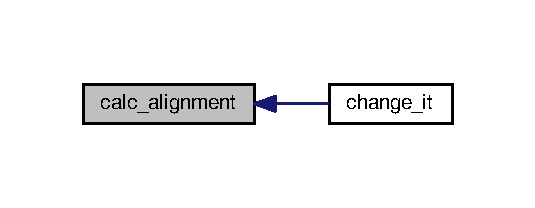
\includegraphics[width=257pt]{_parametric_2_starling-_simulation_2src_2properties_8cpp_a3df27269938df0adf292262c2ea8284d_icgraph}
\end{center}
\end{figure}


\index{Parametric/\+Starling-\/\+Simulation/src/properties.\+cpp@{Parametric/\+Starling-\/\+Simulation/src/properties.\+cpp}!calc\+\_\+boundary\+\_\+force@{calc\+\_\+boundary\+\_\+force}}
\index{calc\+\_\+boundary\+\_\+force@{calc\+\_\+boundary\+\_\+force}!Parametric/\+Starling-\/\+Simulation/src/properties.\+cpp@{Parametric/\+Starling-\/\+Simulation/src/properties.\+cpp}}
\subsubsection[{\texorpdfstring{calc\+\_\+boundary\+\_\+force(boid v)}{calc_boundary_force(boid v)}}]{\setlength{\rightskip}{0pt plus 5cm}{\bf tuple} calc\+\_\+boundary\+\_\+force (
\begin{DoxyParamCaption}
\item[{{\bf boid}}]{v}
\end{DoxyParamCaption}
)}\hypertarget{_parametric_2_starling-_simulation_2src_2properties_8cpp_abee90e2e93e750da724975805408daf0}{}\label{_parametric_2_starling-_simulation_2src_2properties_8cpp_abee90e2e93e750da724975805408daf0}


Definition at line 67 of file properties.\+cpp.



Here is the call graph for this function\+:
\nopagebreak
\begin{figure}[H]
\begin{center}
\leavevmode
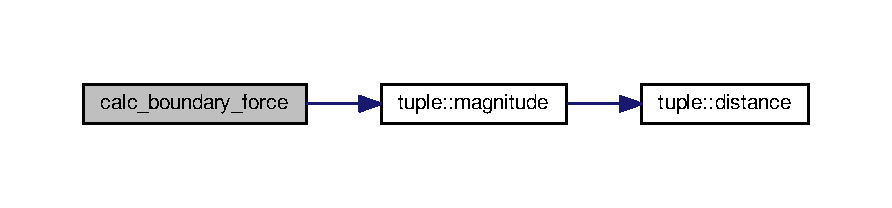
\includegraphics[width=350pt]{_parametric_2_starling-_simulation_2src_2properties_8cpp_abee90e2e93e750da724975805408daf0_cgraph}
\end{center}
\end{figure}




Here is the caller graph for this function\+:
\nopagebreak
\begin{figure}[H]
\begin{center}
\leavevmode
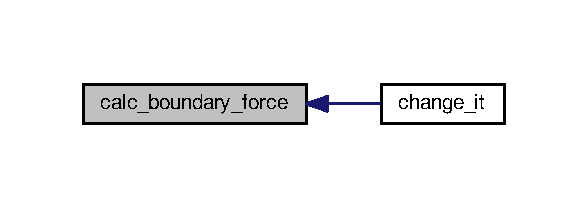
\includegraphics[width=282pt]{_parametric_2_starling-_simulation_2src_2properties_8cpp_abee90e2e93e750da724975805408daf0_icgraph}
\end{center}
\end{figure}


\index{Parametric/\+Starling-\/\+Simulation/src/properties.\+cpp@{Parametric/\+Starling-\/\+Simulation/src/properties.\+cpp}!calc\+\_\+cohesive@{calc\+\_\+cohesive}}
\index{calc\+\_\+cohesive@{calc\+\_\+cohesive}!Parametric/\+Starling-\/\+Simulation/src/properties.\+cpp@{Parametric/\+Starling-\/\+Simulation/src/properties.\+cpp}}
\subsubsection[{\texorpdfstring{calc\+\_\+cohesive(std\+::vector$<$ int $>$ neighbours, int n, std\+::vector$<$ boid $>$ v)}{calc_cohesive(std::vector< int > neighbours, int n, std::vector< boid > v)}}]{\setlength{\rightskip}{0pt plus 5cm}{\bf tuple} calc\+\_\+cohesive (
\begin{DoxyParamCaption}
\item[{std\+::vector$<$ int $>$}]{neighbours, }
\item[{int}]{n, }
\item[{std\+::vector$<$ {\bf boid} $>$}]{v}
\end{DoxyParamCaption}
)}\hypertarget{_parametric_2_starling-_simulation_2src_2properties_8cpp_afa110bb08efe1a435060b69cc946076c}{}\label{_parametric_2_starling-_simulation_2src_2properties_8cpp_afa110bb08efe1a435060b69cc946076c}


Definition at line 39 of file properties.\+cpp.



Here is the call graph for this function\+:
\nopagebreak
\begin{figure}[H]
\begin{center}
\leavevmode
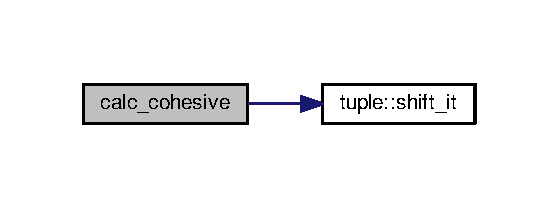
\includegraphics[width=268pt]{_parametric_2_starling-_simulation_2src_2properties_8cpp_afa110bb08efe1a435060b69cc946076c_cgraph}
\end{center}
\end{figure}




Here is the caller graph for this function\+:
\nopagebreak
\begin{figure}[H]
\begin{center}
\leavevmode
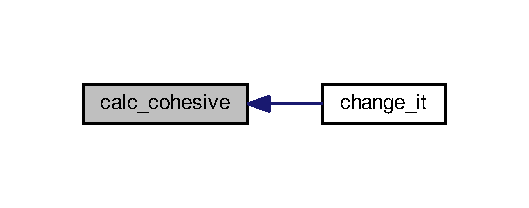
\includegraphics[width=254pt]{_parametric_2_starling-_simulation_2src_2properties_8cpp_afa110bb08efe1a435060b69cc946076c_icgraph}
\end{center}
\end{figure}


\index{Parametric/\+Starling-\/\+Simulation/src/properties.\+cpp@{Parametric/\+Starling-\/\+Simulation/src/properties.\+cpp}!calc\+\_\+separation@{calc\+\_\+separation}}
\index{calc\+\_\+separation@{calc\+\_\+separation}!Parametric/\+Starling-\/\+Simulation/src/properties.\+cpp@{Parametric/\+Starling-\/\+Simulation/src/properties.\+cpp}}
\subsubsection[{\texorpdfstring{calc\+\_\+separation(std\+::vector$<$ int $>$ neighbours, int n, std\+::vector$<$ boid $>$ v)}{calc_separation(std::vector< int > neighbours, int n, std::vector< boid > v)}}]{\setlength{\rightskip}{0pt plus 5cm}{\bf tuple} calc\+\_\+separation (
\begin{DoxyParamCaption}
\item[{std\+::vector$<$ int $>$}]{neighbours, }
\item[{int}]{n, }
\item[{std\+::vector$<$ {\bf boid} $>$}]{v}
\end{DoxyParamCaption}
)}\hypertarget{_parametric_2_starling-_simulation_2src_2properties_8cpp_a50ac6a9e8234630a5ed0b55158cd2e5e}{}\label{_parametric_2_starling-_simulation_2src_2properties_8cpp_a50ac6a9e8234630a5ed0b55158cd2e5e}


Definition at line 53 of file properties.\+cpp.



Here is the call graph for this function\+:
\nopagebreak
\begin{figure}[H]
\begin{center}
\leavevmode
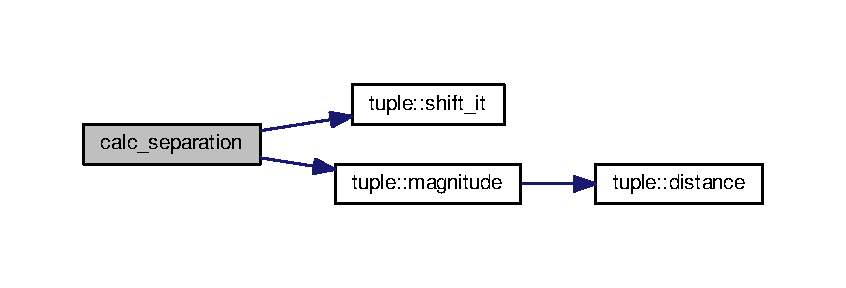
\includegraphics[width=350pt]{_parametric_2_starling-_simulation_2src_2properties_8cpp_a50ac6a9e8234630a5ed0b55158cd2e5e_cgraph}
\end{center}
\end{figure}




Here is the caller graph for this function\+:
\nopagebreak
\begin{figure}[H]
\begin{center}
\leavevmode
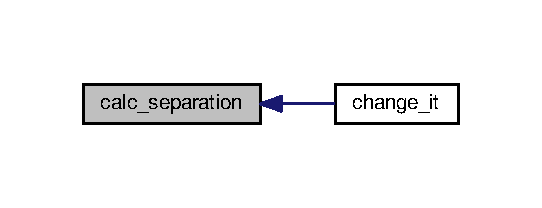
\includegraphics[width=260pt]{_parametric_2_starling-_simulation_2src_2properties_8cpp_a50ac6a9e8234630a5ed0b55158cd2e5e_icgraph}
\end{center}
\end{figure}


\index{Parametric/\+Starling-\/\+Simulation/src/properties.\+cpp@{Parametric/\+Starling-\/\+Simulation/src/properties.\+cpp}!change\+\_\+it@{change\+\_\+it}}
\index{change\+\_\+it@{change\+\_\+it}!Parametric/\+Starling-\/\+Simulation/src/properties.\+cpp@{Parametric/\+Starling-\/\+Simulation/src/properties.\+cpp}}
\subsubsection[{\texorpdfstring{change\+\_\+it(std\+::vector$<$ boid $>$ \&v)}{change_it(std::vector< boid > &v)}}]{\setlength{\rightskip}{0pt plus 5cm}void change\+\_\+it (
\begin{DoxyParamCaption}
\item[{std\+::vector$<$ {\bf boid} $>$ \&}]{v}
\end{DoxyParamCaption}
)}\hypertarget{_parametric_2_starling-_simulation_2src_2properties_8cpp_a0997f2a51d68a3d4a7d8ae247af76cab}{}\label{_parametric_2_starling-_simulation_2src_2properties_8cpp_a0997f2a51d68a3d4a7d8ae247af76cab}


Definition at line 208 of file properties.\+cpp.



Here is the call graph for this function\+:
\nopagebreak
\begin{figure}[H]
\begin{center}
\leavevmode
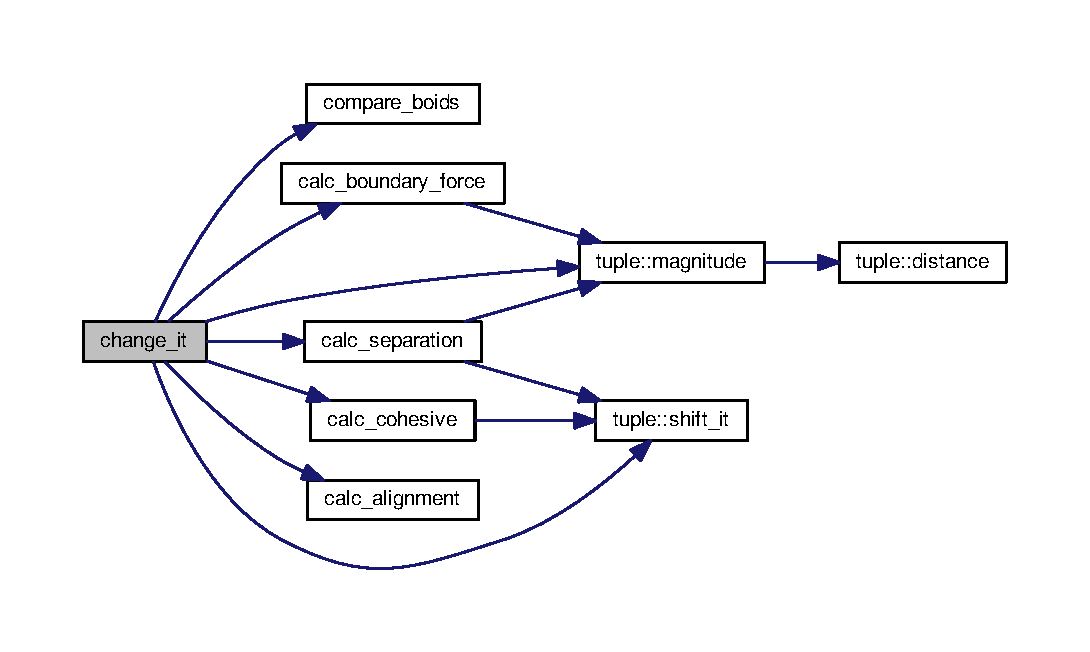
\includegraphics[width=350pt]{_parametric_2_starling-_simulation_2src_2properties_8cpp_a0997f2a51d68a3d4a7d8ae247af76cab_cgraph}
\end{center}
\end{figure}


\index{Parametric/\+Starling-\/\+Simulation/src/properties.\+cpp@{Parametric/\+Starling-\/\+Simulation/src/properties.\+cpp}!compare\+\_\+boids@{compare\+\_\+boids}}
\index{compare\+\_\+boids@{compare\+\_\+boids}!Parametric/\+Starling-\/\+Simulation/src/properties.\+cpp@{Parametric/\+Starling-\/\+Simulation/src/properties.\+cpp}}
\subsubsection[{\texorpdfstring{compare\+\_\+boids(boid lhs, boid rhs)}{compare_boids(boid lhs, boid rhs)}}]{\setlength{\rightskip}{0pt plus 5cm}bool compare\+\_\+boids (
\begin{DoxyParamCaption}
\item[{{\bf boid}}]{lhs, }
\item[{{\bf boid}}]{rhs}
\end{DoxyParamCaption}
)}\hypertarget{_parametric_2_starling-_simulation_2src_2properties_8cpp_a7710f08e0d0c5ec292c8527e64d91813}{}\label{_parametric_2_starling-_simulation_2src_2properties_8cpp_a7710f08e0d0c5ec292c8527e64d91813}


Definition at line 197 of file properties.\+cpp.



Here is the caller graph for this function\+:
\nopagebreak
\begin{figure}[H]
\begin{center}
\leavevmode
\includegraphics[width=258pt]{_parametric_2_starling-_simulation_2src_2properties_8cpp_a7710f08e0d0c5ec292c8527e64d91813_icgraph}
\end{center}
\end{figure}


\index{Parametric/\+Starling-\/\+Simulation/src/properties.\+cpp@{Parametric/\+Starling-\/\+Simulation/src/properties.\+cpp}!give\+\_\+neighbours@{give\+\_\+neighbours}}
\index{give\+\_\+neighbours@{give\+\_\+neighbours}!Parametric/\+Starling-\/\+Simulation/src/properties.\+cpp@{Parametric/\+Starling-\/\+Simulation/src/properties.\+cpp}}
\subsubsection[{\texorpdfstring{give\+\_\+neighbours(int n, std\+::vector$<$ boid $>$ v)}{give_neighbours(int n, std::vector< boid > v)}}]{\setlength{\rightskip}{0pt plus 5cm}std\+::vector$<$int$>$ give\+\_\+neighbours (
\begin{DoxyParamCaption}
\item[{int}]{n, }
\item[{std\+::vector$<$ {\bf boid} $>$}]{v}
\end{DoxyParamCaption}
)}\hypertarget{_parametric_2_starling-_simulation_2src_2properties_8cpp_a8a274a3ed40ef9c3fb2eea8f2f2f8358}{}\label{_parametric_2_starling-_simulation_2src_2properties_8cpp_a8a274a3ed40ef9c3fb2eea8f2f2f8358}


Definition at line 18 of file properties.\+cpp.



Here is the caller graph for this function\+:
\nopagebreak
\begin{figure}[H]
\begin{center}
\leavevmode
\includegraphics[width=350pt]{_parametric_2_starling-_simulation_2src_2properties_8cpp_a8a274a3ed40ef9c3fb2eea8f2f2f8358_icgraph}
\end{center}
\end{figure}



\hypertarget{src_2properties_8cpp}{}\section{src/properties.cpp File Reference}
\label{src_2properties_8cpp}\index{src/properties.\+cpp@{src/properties.\+cpp}}
{\ttfamily \#include \char`\"{}../include/properties.\+h\char`\"{}}\\*
{\ttfamily \#include $<$bits/stdc++.\+h$>$}\\*
Include dependency graph for properties.\+cpp\+:
\nopagebreak
\begin{figure}[H]
\begin{center}
\leavevmode
\includegraphics[width=252pt]{src_2properties_8cpp__incl}
\end{center}
\end{figure}
\subsection*{Macros}
\begin{DoxyCompactItemize}
\item 
\#define \hyperlink{src_2properties_8cpp_ab16f7f055bbbd643b9510d1bd42eb4dc}{cohesion\+\_\+coeff}~3.\+0
\item 
\#define \hyperlink{src_2properties_8cpp_a7f599c3f3ac600fcccbd330b534e48ae}{separation\+\_\+coeff}~2.\+0
\item 
\#define \hyperlink{src_2properties_8cpp_a9439746dd157dbb69b93e084d1edfb01}{alignment\+\_\+coeff}~0.\+5
\item 
\#define \hyperlink{src_2properties_8cpp_aada98d3e75b15aaf71743634702209b2}{inertia\+\_\+coeff}~0.\+1
\item 
\#define \hyperlink{src_2properties_8cpp_a77da7eab1cc4cbb2c82f162c70fbc5c6}{boundary\+\_\+repulsion\+\_\+coeff}~0.\+8
\item 
\#define \hyperlink{src_2properties_8cpp_ae3ae4055677d82207f6578facdb0fc9f}{wall\+\_\+coeff}~50.\+0
\item 
\#define \hyperlink{src_2properties_8cpp_aa1f49d89b055225bac6ab75db254c1b3}{wall\+\_\+coeff\+\_\+near}~5.\+0
\item 
\#define \hyperlink{src_2properties_8cpp_a77e76b711036e5e2fcea28729e200658}{radius}~80.\+0
\item 
\#define \hyperlink{src_2properties_8cpp_ae3a4f0027a70e328f9ed18819cb867c7}{no\+\_\+of\+\_\+neighbours}~15
\end{DoxyCompactItemize}
\subsection*{Functions}
\begin{DoxyCompactItemize}
\item 
std\+::vector$<$ int $>$ \hyperlink{src_2properties_8cpp_a8a274a3ed40ef9c3fb2eea8f2f2f8358}{give\+\_\+neighbours} (int n, std\+::vector$<$ \hyperlink{classboid}{boid} $>$ \hyperlink{src_2main_8cpp_a1d5a718f1d6b42141bc3a6834be5e420}{v})
\item 
\hyperlink{classtuple}{tuple} \hyperlink{src_2properties_8cpp_afa110bb08efe1a435060b69cc946076c}{calc\+\_\+cohesive} (std\+::vector$<$ int $>$ neighbours, int n, std\+::vector$<$ \hyperlink{classboid}{boid} $>$ \hyperlink{src_2main_8cpp_a1d5a718f1d6b42141bc3a6834be5e420}{v})
\item 
\hyperlink{classtuple}{tuple} \hyperlink{src_2properties_8cpp_a50ac6a9e8234630a5ed0b55158cd2e5e}{calc\+\_\+separation} (std\+::vector$<$ int $>$ neighbours, int n, std\+::vector$<$ \hyperlink{classboid}{boid} $>$ \hyperlink{src_2main_8cpp_a1d5a718f1d6b42141bc3a6834be5e420}{v})
\item 
\hyperlink{classtuple}{tuple} \hyperlink{src_2properties_8cpp_abee90e2e93e750da724975805408daf0}{calc\+\_\+boundary\+\_\+force} (\hyperlink{classboid}{boid} \hyperlink{src_2main_8cpp_a1d5a718f1d6b42141bc3a6834be5e420}{v})
\item 
\hyperlink{classtuple}{tuple} \hyperlink{src_2properties_8cpp_a3df27269938df0adf292262c2ea8284d}{calc\+\_\+alignment} (std\+::vector$<$ int $>$ neighbours, int n, std\+::vector$<$ \hyperlink{classboid}{boid} $>$ \hyperlink{src_2main_8cpp_a1d5a718f1d6b42141bc3a6834be5e420}{v})
\item 
void \hyperlink{src_2properties_8cpp_a0997f2a51d68a3d4a7d8ae247af76cab}{change\+\_\+it} (std\+::vector$<$ \hyperlink{classboid}{boid} $>$ \&\hyperlink{src_2main_8cpp_a1d5a718f1d6b42141bc3a6834be5e420}{v})
\end{DoxyCompactItemize}


\subsection{Macro Definition Documentation}
\index{src/properties.\+cpp@{src/properties.\+cpp}!alignment\+\_\+coeff@{alignment\+\_\+coeff}}
\index{alignment\+\_\+coeff@{alignment\+\_\+coeff}!src/properties.\+cpp@{src/properties.\+cpp}}
\subsubsection[{\texorpdfstring{alignment\+\_\+coeff}{alignment_coeff}}]{\setlength{\rightskip}{0pt plus 5cm}\#define alignment\+\_\+coeff~0.\+5}\hypertarget{src_2properties_8cpp_a9439746dd157dbb69b93e084d1edfb01}{}\label{src_2properties_8cpp_a9439746dd157dbb69b93e084d1edfb01}


Definition at line 6 of file properties.\+cpp.

\index{src/properties.\+cpp@{src/properties.\+cpp}!boundary\+\_\+repulsion\+\_\+coeff@{boundary\+\_\+repulsion\+\_\+coeff}}
\index{boundary\+\_\+repulsion\+\_\+coeff@{boundary\+\_\+repulsion\+\_\+coeff}!src/properties.\+cpp@{src/properties.\+cpp}}
\subsubsection[{\texorpdfstring{boundary\+\_\+repulsion\+\_\+coeff}{boundary_repulsion_coeff}}]{\setlength{\rightskip}{0pt plus 5cm}\#define boundary\+\_\+repulsion\+\_\+coeff~0.\+8}\hypertarget{src_2properties_8cpp_a77da7eab1cc4cbb2c82f162c70fbc5c6}{}\label{src_2properties_8cpp_a77da7eab1cc4cbb2c82f162c70fbc5c6}


Definition at line 8 of file properties.\+cpp.

\index{src/properties.\+cpp@{src/properties.\+cpp}!cohesion\+\_\+coeff@{cohesion\+\_\+coeff}}
\index{cohesion\+\_\+coeff@{cohesion\+\_\+coeff}!src/properties.\+cpp@{src/properties.\+cpp}}
\subsubsection[{\texorpdfstring{cohesion\+\_\+coeff}{cohesion_coeff}}]{\setlength{\rightskip}{0pt plus 5cm}\#define cohesion\+\_\+coeff~3.\+0}\hypertarget{src_2properties_8cpp_ab16f7f055bbbd643b9510d1bd42eb4dc}{}\label{src_2properties_8cpp_ab16f7f055bbbd643b9510d1bd42eb4dc}


Definition at line 4 of file properties.\+cpp.

\index{src/properties.\+cpp@{src/properties.\+cpp}!inertia\+\_\+coeff@{inertia\+\_\+coeff}}
\index{inertia\+\_\+coeff@{inertia\+\_\+coeff}!src/properties.\+cpp@{src/properties.\+cpp}}
\subsubsection[{\texorpdfstring{inertia\+\_\+coeff}{inertia_coeff}}]{\setlength{\rightskip}{0pt plus 5cm}\#define inertia\+\_\+coeff~0.\+1}\hypertarget{src_2properties_8cpp_aada98d3e75b15aaf71743634702209b2}{}\label{src_2properties_8cpp_aada98d3e75b15aaf71743634702209b2}


Definition at line 7 of file properties.\+cpp.

\index{src/properties.\+cpp@{src/properties.\+cpp}!no\+\_\+of\+\_\+neighbours@{no\+\_\+of\+\_\+neighbours}}
\index{no\+\_\+of\+\_\+neighbours@{no\+\_\+of\+\_\+neighbours}!src/properties.\+cpp@{src/properties.\+cpp}}
\subsubsection[{\texorpdfstring{no\+\_\+of\+\_\+neighbours}{no_of_neighbours}}]{\setlength{\rightskip}{0pt plus 5cm}\#define no\+\_\+of\+\_\+neighbours~15}\hypertarget{src_2properties_8cpp_ae3a4f0027a70e328f9ed18819cb867c7}{}\label{src_2properties_8cpp_ae3a4f0027a70e328f9ed18819cb867c7}


Definition at line 12 of file properties.\+cpp.

\index{src/properties.\+cpp@{src/properties.\+cpp}!radius@{radius}}
\index{radius@{radius}!src/properties.\+cpp@{src/properties.\+cpp}}
\subsubsection[{\texorpdfstring{radius}{radius}}]{\setlength{\rightskip}{0pt plus 5cm}\#define radius~80.\+0}\hypertarget{src_2properties_8cpp_a77e76b711036e5e2fcea28729e200658}{}\label{src_2properties_8cpp_a77e76b711036e5e2fcea28729e200658}


Definition at line 11 of file properties.\+cpp.

\index{src/properties.\+cpp@{src/properties.\+cpp}!separation\+\_\+coeff@{separation\+\_\+coeff}}
\index{separation\+\_\+coeff@{separation\+\_\+coeff}!src/properties.\+cpp@{src/properties.\+cpp}}
\subsubsection[{\texorpdfstring{separation\+\_\+coeff}{separation_coeff}}]{\setlength{\rightskip}{0pt plus 5cm}\#define separation\+\_\+coeff~2.\+0}\hypertarget{src_2properties_8cpp_a7f599c3f3ac600fcccbd330b534e48ae}{}\label{src_2properties_8cpp_a7f599c3f3ac600fcccbd330b534e48ae}


Definition at line 5 of file properties.\+cpp.

\index{src/properties.\+cpp@{src/properties.\+cpp}!wall\+\_\+coeff@{wall\+\_\+coeff}}
\index{wall\+\_\+coeff@{wall\+\_\+coeff}!src/properties.\+cpp@{src/properties.\+cpp}}
\subsubsection[{\texorpdfstring{wall\+\_\+coeff}{wall_coeff}}]{\setlength{\rightskip}{0pt plus 5cm}\#define wall\+\_\+coeff~50.\+0}\hypertarget{src_2properties_8cpp_ae3ae4055677d82207f6578facdb0fc9f}{}\label{src_2properties_8cpp_ae3ae4055677d82207f6578facdb0fc9f}


Definition at line 9 of file properties.\+cpp.

\index{src/properties.\+cpp@{src/properties.\+cpp}!wall\+\_\+coeff\+\_\+near@{wall\+\_\+coeff\+\_\+near}}
\index{wall\+\_\+coeff\+\_\+near@{wall\+\_\+coeff\+\_\+near}!src/properties.\+cpp@{src/properties.\+cpp}}
\subsubsection[{\texorpdfstring{wall\+\_\+coeff\+\_\+near}{wall_coeff_near}}]{\setlength{\rightskip}{0pt plus 5cm}\#define wall\+\_\+coeff\+\_\+near~5.\+0}\hypertarget{src_2properties_8cpp_aa1f49d89b055225bac6ab75db254c1b3}{}\label{src_2properties_8cpp_aa1f49d89b055225bac6ab75db254c1b3}


Definition at line 10 of file properties.\+cpp.



\subsection{Function Documentation}
\index{src/properties.\+cpp@{src/properties.\+cpp}!calc\+\_\+alignment@{calc\+\_\+alignment}}
\index{calc\+\_\+alignment@{calc\+\_\+alignment}!src/properties.\+cpp@{src/properties.\+cpp}}
\subsubsection[{\texorpdfstring{calc\+\_\+alignment(std\+::vector$<$ int $>$ neighbours, int n, std\+::vector$<$ boid $>$ v)}{calc_alignment(std::vector< int > neighbours, int n, std::vector< boid > v)}}]{\setlength{\rightskip}{0pt plus 5cm}{\bf tuple} calc\+\_\+alignment (
\begin{DoxyParamCaption}
\item[{std\+::vector$<$ int $>$}]{neighbours, }
\item[{int}]{n, }
\item[{std\+::vector$<$ {\bf boid} $>$}]{v}
\end{DoxyParamCaption}
)}\hypertarget{src_2properties_8cpp_a3df27269938df0adf292262c2ea8284d}{}\label{src_2properties_8cpp_a3df27269938df0adf292262c2ea8284d}


Definition at line 182 of file properties.\+cpp.

\index{src/properties.\+cpp@{src/properties.\+cpp}!calc\+\_\+boundary\+\_\+force@{calc\+\_\+boundary\+\_\+force}}
\index{calc\+\_\+boundary\+\_\+force@{calc\+\_\+boundary\+\_\+force}!src/properties.\+cpp@{src/properties.\+cpp}}
\subsubsection[{\texorpdfstring{calc\+\_\+boundary\+\_\+force(boid v)}{calc_boundary_force(boid v)}}]{\setlength{\rightskip}{0pt plus 5cm}{\bf tuple} calc\+\_\+boundary\+\_\+force (
\begin{DoxyParamCaption}
\item[{{\bf boid}}]{v}
\end{DoxyParamCaption}
)}\hypertarget{src_2properties_8cpp_abee90e2e93e750da724975805408daf0}{}\label{src_2properties_8cpp_abee90e2e93e750da724975805408daf0}


Definition at line 65 of file properties.\+cpp.



Here is the call graph for this function\+:
\nopagebreak
\begin{figure}[H]
\begin{center}
\leavevmode
\includegraphics[width=350pt]{src_2properties_8cpp_abee90e2e93e750da724975805408daf0_cgraph}
\end{center}
\end{figure}


\index{src/properties.\+cpp@{src/properties.\+cpp}!calc\+\_\+cohesive@{calc\+\_\+cohesive}}
\index{calc\+\_\+cohesive@{calc\+\_\+cohesive}!src/properties.\+cpp@{src/properties.\+cpp}}
\subsubsection[{\texorpdfstring{calc\+\_\+cohesive(std\+::vector$<$ int $>$ neighbours, int n, std\+::vector$<$ boid $>$ v)}{calc_cohesive(std::vector< int > neighbours, int n, std::vector< boid > v)}}]{\setlength{\rightskip}{0pt plus 5cm}{\bf tuple} calc\+\_\+cohesive (
\begin{DoxyParamCaption}
\item[{std\+::vector$<$ int $>$}]{neighbours, }
\item[{int}]{n, }
\item[{std\+::vector$<$ {\bf boid} $>$}]{v}
\end{DoxyParamCaption}
)}\hypertarget{src_2properties_8cpp_afa110bb08efe1a435060b69cc946076c}{}\label{src_2properties_8cpp_afa110bb08efe1a435060b69cc946076c}


Definition at line 37 of file properties.\+cpp.



Here is the call graph for this function\+:
\nopagebreak
\begin{figure}[H]
\begin{center}
\leavevmode
\includegraphics[width=268pt]{src_2properties_8cpp_afa110bb08efe1a435060b69cc946076c_cgraph}
\end{center}
\end{figure}


\index{src/properties.\+cpp@{src/properties.\+cpp}!calc\+\_\+separation@{calc\+\_\+separation}}
\index{calc\+\_\+separation@{calc\+\_\+separation}!src/properties.\+cpp@{src/properties.\+cpp}}
\subsubsection[{\texorpdfstring{calc\+\_\+separation(std\+::vector$<$ int $>$ neighbours, int n, std\+::vector$<$ boid $>$ v)}{calc_separation(std::vector< int > neighbours, int n, std::vector< boid > v)}}]{\setlength{\rightskip}{0pt plus 5cm}{\bf tuple} calc\+\_\+separation (
\begin{DoxyParamCaption}
\item[{std\+::vector$<$ int $>$}]{neighbours, }
\item[{int}]{n, }
\item[{std\+::vector$<$ {\bf boid} $>$}]{v}
\end{DoxyParamCaption}
)}\hypertarget{src_2properties_8cpp_a50ac6a9e8234630a5ed0b55158cd2e5e}{}\label{src_2properties_8cpp_a50ac6a9e8234630a5ed0b55158cd2e5e}


Definition at line 51 of file properties.\+cpp.



Here is the call graph for this function\+:
\nopagebreak
\begin{figure}[H]
\begin{center}
\leavevmode
\includegraphics[width=350pt]{src_2properties_8cpp_a50ac6a9e8234630a5ed0b55158cd2e5e_cgraph}
\end{center}
\end{figure}


\index{src/properties.\+cpp@{src/properties.\+cpp}!change\+\_\+it@{change\+\_\+it}}
\index{change\+\_\+it@{change\+\_\+it}!src/properties.\+cpp@{src/properties.\+cpp}}
\subsubsection[{\texorpdfstring{change\+\_\+it(std\+::vector$<$ boid $>$ \&v)}{change_it(std::vector< boid > &v)}}]{\setlength{\rightskip}{0pt plus 5cm}void change\+\_\+it (
\begin{DoxyParamCaption}
\item[{std\+::vector$<$ {\bf boid} $>$ \&}]{v}
\end{DoxyParamCaption}
)}\hypertarget{src_2properties_8cpp_a0997f2a51d68a3d4a7d8ae247af76cab}{}\label{src_2properties_8cpp_a0997f2a51d68a3d4a7d8ae247af76cab}


Definition at line 195 of file properties.\+cpp.



Here is the call graph for this function\+:
\nopagebreak
\begin{figure}[H]
\begin{center}
\leavevmode
\includegraphics[width=350pt]{src_2properties_8cpp_a0997f2a51d68a3d4a7d8ae247af76cab_cgraph}
\end{center}
\end{figure}




Here is the caller graph for this function\+:
\nopagebreak
\begin{figure}[H]
\begin{center}
\leavevmode
\includegraphics[width=278pt]{src_2properties_8cpp_a0997f2a51d68a3d4a7d8ae247af76cab_icgraph}
\end{center}
\end{figure}


\index{src/properties.\+cpp@{src/properties.\+cpp}!give\+\_\+neighbours@{give\+\_\+neighbours}}
\index{give\+\_\+neighbours@{give\+\_\+neighbours}!src/properties.\+cpp@{src/properties.\+cpp}}
\subsubsection[{\texorpdfstring{give\+\_\+neighbours(int n, std\+::vector$<$ boid $>$ v)}{give_neighbours(int n, std::vector< boid > v)}}]{\setlength{\rightskip}{0pt plus 5cm}std\+::vector$<$int$>$ give\+\_\+neighbours (
\begin{DoxyParamCaption}
\item[{int}]{n, }
\item[{std\+::vector$<$ {\bf boid} $>$}]{v}
\end{DoxyParamCaption}
)}\hypertarget{src_2properties_8cpp_a8a274a3ed40ef9c3fb2eea8f2f2f8358}{}\label{src_2properties_8cpp_a8a274a3ed40ef9c3fb2eea8f2f2f8358}


Definition at line 16 of file properties.\+cpp.


\hypertarget{animation_8cpp}{}\section{src/animation.cpp File Reference}
\label{animation_8cpp}\index{src/animation.\+cpp@{src/animation.\+cpp}}
{\ttfamily \#include $<$G\+L/glut.\+h$>$}\\*
Include dependency graph for animation.\+cpp\+:
\nopagebreak
\begin{figure}[H]
\begin{center}
\leavevmode
\includegraphics[width=174pt]{animation_8cpp__incl}
\end{center}
\end{figure}
\subsection*{Functions}
\begin{DoxyCompactItemize}
\item 
void \hyperlink{animation_8cpp_a2858154e2009b0e6e616f313177762bc}{init} (void)
\item 
void \hyperlink{animation_8cpp_a4ea013001a5fb47853d0fab8f8de35cd}{display} (void)
\item 
void \hyperlink{animation_8cpp_a26d4b6f6d996a0f15ed6b7282a794a49}{spin\+Display} (void)
\item 
void \hyperlink{animation_8cpp_acc1ffe65e6869931318610cae7210078}{reshape} (int \hyperlink{src_2main_8cpp_aac374e320caaadeca4874add33b62af2}{w}, int \hyperlink{src_2main_8cpp_a16611451551e3d15916bae723c3f59f7}{h})
\item 
void \hyperlink{animation_8cpp_ac76a5d78172a826cd6ee9512b89a86c0}{mouse} (int button, int state, int x, int y)
\item 
int \hyperlink{animation_8cpp_a3c04138a5bfe5d72780bb7e82a18e627}{main} (int argc, char $\ast$$\ast$argv)
\end{DoxyCompactItemize}


\subsection{Function Documentation}
\index{animation.\+cpp@{animation.\+cpp}!display@{display}}
\index{display@{display}!animation.\+cpp@{animation.\+cpp}}
\subsubsection[{\texorpdfstring{display(void)}{display(void)}}]{\setlength{\rightskip}{0pt plus 5cm}void display (
\begin{DoxyParamCaption}
\item[{void}]{}
\end{DoxyParamCaption}
)}\hypertarget{animation_8cpp_a4ea013001a5fb47853d0fab8f8de35cd}{}\label{animation_8cpp_a4ea013001a5fb47853d0fab8f8de35cd}


Definition at line 9 of file animation.\+cpp.



Here is the caller graph for this function\+:
\nopagebreak
\begin{figure}[H]
\begin{center}
\leavevmode
\includegraphics[width=201pt]{animation_8cpp_a4ea013001a5fb47853d0fab8f8de35cd_icgraph}
\end{center}
\end{figure}


\index{animation.\+cpp@{animation.\+cpp}!init@{init}}
\index{init@{init}!animation.\+cpp@{animation.\+cpp}}
\subsubsection[{\texorpdfstring{init(void)}{init(void)}}]{\setlength{\rightskip}{0pt plus 5cm}void init (
\begin{DoxyParamCaption}
\item[{void}]{}
\end{DoxyParamCaption}
)}\hypertarget{animation_8cpp_a2858154e2009b0e6e616f313177762bc}{}\label{animation_8cpp_a2858154e2009b0e6e616f313177762bc}


Definition at line 4 of file animation.\+cpp.



Here is the caller graph for this function\+:
\nopagebreak
\begin{figure}[H]
\begin{center}
\leavevmode
\includegraphics[width=183pt]{animation_8cpp_a2858154e2009b0e6e616f313177762bc_icgraph}
\end{center}
\end{figure}


\index{animation.\+cpp@{animation.\+cpp}!main@{main}}
\index{main@{main}!animation.\+cpp@{animation.\+cpp}}
\subsubsection[{\texorpdfstring{main(int argc, char $\ast$$\ast$argv)}{main(int argc, char **argv)}}]{\setlength{\rightskip}{0pt plus 5cm}int main (
\begin{DoxyParamCaption}
\item[{int}]{argc, }
\item[{char $\ast$$\ast$}]{argv}
\end{DoxyParamCaption}
)}\hypertarget{animation_8cpp_a3c04138a5bfe5d72780bb7e82a18e627}{}\label{animation_8cpp_a3c04138a5bfe5d72780bb7e82a18e627}


Definition at line 54 of file animation.\+cpp.



Here is the call graph for this function\+:
\nopagebreak
\begin{figure}[H]
\begin{center}
\leavevmode
\includegraphics[width=309pt]{animation_8cpp_a3c04138a5bfe5d72780bb7e82a18e627_cgraph}
\end{center}
\end{figure}


\index{animation.\+cpp@{animation.\+cpp}!mouse@{mouse}}
\index{mouse@{mouse}!animation.\+cpp@{animation.\+cpp}}
\subsubsection[{\texorpdfstring{mouse(int button, int state, int x, int y)}{mouse(int button, int state, int x, int y)}}]{\setlength{\rightskip}{0pt plus 5cm}void mouse (
\begin{DoxyParamCaption}
\item[{int}]{button, }
\item[{int}]{state, }
\item[{int}]{x, }
\item[{int}]{y}
\end{DoxyParamCaption}
)}\hypertarget{animation_8cpp_ac76a5d78172a826cd6ee9512b89a86c0}{}\label{animation_8cpp_ac76a5d78172a826cd6ee9512b89a86c0}


Definition at line 37 of file animation.\+cpp.



Here is the call graph for this function\+:
\nopagebreak
\begin{figure}[H]
\begin{center}
\leavevmode
\includegraphics[width=230pt]{animation_8cpp_ac76a5d78172a826cd6ee9512b89a86c0_cgraph}
\end{center}
\end{figure}




Here is the caller graph for this function\+:
\nopagebreak
\begin{figure}[H]
\begin{center}
\leavevmode
\includegraphics[width=200pt]{animation_8cpp_ac76a5d78172a826cd6ee9512b89a86c0_icgraph}
\end{center}
\end{figure}


\index{animation.\+cpp@{animation.\+cpp}!reshape@{reshape}}
\index{reshape@{reshape}!animation.\+cpp@{animation.\+cpp}}
\subsubsection[{\texorpdfstring{reshape(int w, int h)}{reshape(int w, int h)}}]{\setlength{\rightskip}{0pt plus 5cm}void reshape (
\begin{DoxyParamCaption}
\item[{int}]{w, }
\item[{int}]{h}
\end{DoxyParamCaption}
)}\hypertarget{animation_8cpp_acc1ffe65e6869931318610cae7210078}{}\label{animation_8cpp_acc1ffe65e6869931318610cae7210078}


Definition at line 27 of file animation.\+cpp.



Here is the caller graph for this function\+:
\nopagebreak
\begin{figure}[H]
\begin{center}
\leavevmode
\includegraphics[width=205pt]{animation_8cpp_acc1ffe65e6869931318610cae7210078_icgraph}
\end{center}
\end{figure}


\index{animation.\+cpp@{animation.\+cpp}!spin\+Display@{spin\+Display}}
\index{spin\+Display@{spin\+Display}!animation.\+cpp@{animation.\+cpp}}
\subsubsection[{\texorpdfstring{spin\+Display(void)}{spinDisplay(void)}}]{\setlength{\rightskip}{0pt plus 5cm}void spin\+Display (
\begin{DoxyParamCaption}
\item[{void}]{}
\end{DoxyParamCaption}
)}\hypertarget{animation_8cpp_a26d4b6f6d996a0f15ed6b7282a794a49}{}\label{animation_8cpp_a26d4b6f6d996a0f15ed6b7282a794a49}


Definition at line 20 of file animation.\+cpp.



Here is the caller graph for this function\+:
\nopagebreak
\begin{figure}[H]
\begin{center}
\leavevmode
\includegraphics[width=304pt]{animation_8cpp_a26d4b6f6d996a0f15ed6b7282a794a49_icgraph}
\end{center}
\end{figure}



%--- End generated contents ---

% Index
\backmatter
\newpage
\phantomsection
\clearemptydoublepage
\addcontentsline{toc}{chapter}{Index}
\printindex

\end{document}
